\documentclass[a4j,12pt,dvipdfmx]{jreport}
\usepackage[top=35mm, bottom=30mm, left=30mm, right=30mm]{geometry}

<<<<<<< HEAD
% \oddsidemargin= 5mm   
\textwidth = 160mm
\textheight = 205mm
% \addtolength{\textheight}{3cm}
% %\addtolength{\textwidth}{1.5cm}
% \topmargin = -5mm
% \headheight = 0mm
% \footskip = 10mm

% % 図形に関する処理
\renewcommand{\topfraction}{1.0}
\renewcommand{\bottomfraction}{1.0}
\renewcommand{\dbltopfraction}{1.0}
\renewcommand{\textfraction}{0.01}
\renewcommand{\floatpagefraction}{1.0}
\renewcommand{\dblfloatpagefraction}{1.0}
\setcounter{topnumber}{5}
\setcounter{bottomnumber}{5}
\setcounter{totalnumber}{10}

=======
>>>>>>> parent of 36117c4 (考察増やした)
\usepackage{url}
\usepackage[dvipdfmx]{graphicx}
\usepackage{amsmath,amsthm,amssymb,ascmac}
\usepackage{fancyhdr}
\usepackage{fancybox}
\usepackage{fancyvrb}
\usepackage[T1]{fontenc}
\usepackage{subcaption}
\usepackage{comment}
\usepackage{here}
\usepackage{float}
\usepackage{booktabs}
\usepackage{makecell}

\renewcommand{\bibname}{参考文献}

\begin{document}
\pagenumbering{roman}
%表紙
\begin{titlepage} \centering
  %\LARGE
  \null \null
  \vspace{10mm}
  令和04年度 卒業研究論文\\
  %\vfill
  \vspace{55.15mm}
  \null
  % 研究題目\\
  {\Large CNNを用いた動画インデックス作成に関する研究}\\
  %\vfill \vfill
  %\vfill
  
  \vspace{87.5mm}
  %{\Large 平成24年2月23日}
  %\vspace{15mm}
  
  \large
  総合工学科 情報システムコース 5年\\[1mm]
  1801113 藤田 晴斗\\[1mm]
  指導教員 総合工学科 藤原 和彦\\
  
  \vspace{16mm}
  {仙台高等専門学校}
  \null

\end{titlepage}

%目次
% \tableofcontents
% \clearpage
\clearpage \tableofcontents
\listoftables
\listoffigures
% \thispagestyle{empty}
% \pagestyle{plain}
% \setcounter{page}{0}


%\setcounter{page}{0}
%\pagenumbering{roman}
%\tableofcontents
%\thispagestyle{empty}
{\clearpage}
\large
\renewcommand{\baselinestretch}{1.1}

\chapter{序論}
\pagenumbering{arabic}
\label{sec:introducion}

\section{研究背景}
近年,スマートフォンや動画ストリーミングサービスの急速な普及に伴い,個人が取り扱う動画の本数が大幅に増加している.
2020年にGoogle社が発表したYouTube(動画ストリーミングサービス)にアップロードされた動画の総時間について,2019年と比較して80%も増加していることがわかった\cite{google_data}.
そこで,個人が取り扱う動画について,より効率的なデータ管理を行うためのシステムが求められていると考えられる.

これまで,動画内で入力した画像と一致するシーンを検索するには,動画の各フレームを画像のように扱い,フレーム同士の各座標の画素値(RGB値)が完全に一致しているものを探す必要があった.
また,動画内から画像の類似シーンを検索しようとしたときには,互いの画素が一致している割合を用いて比較・検討が行われる.
そこで実際の画像(図\ref{fig:hikaku})を用いた類似度の推定を行なってみた.

画像のヒストグラムから類似度を計算するプログラムではこ,の2枚の画像は類似度36%であると推定された.
しかし,構成している物体が同じであるため,類似した画像として扱えるのではないかと考えた.
この仮説のもと,広い意味での類似したシーン検索ができるよう,これまでのRGB値での比較を行うのではなく,画像を構成している物体に着目した比較を行うことができるようなシステム構築を目指した.

\vspace{2zh}
\begin{figure}[htbp]
  \centering
  \fbox{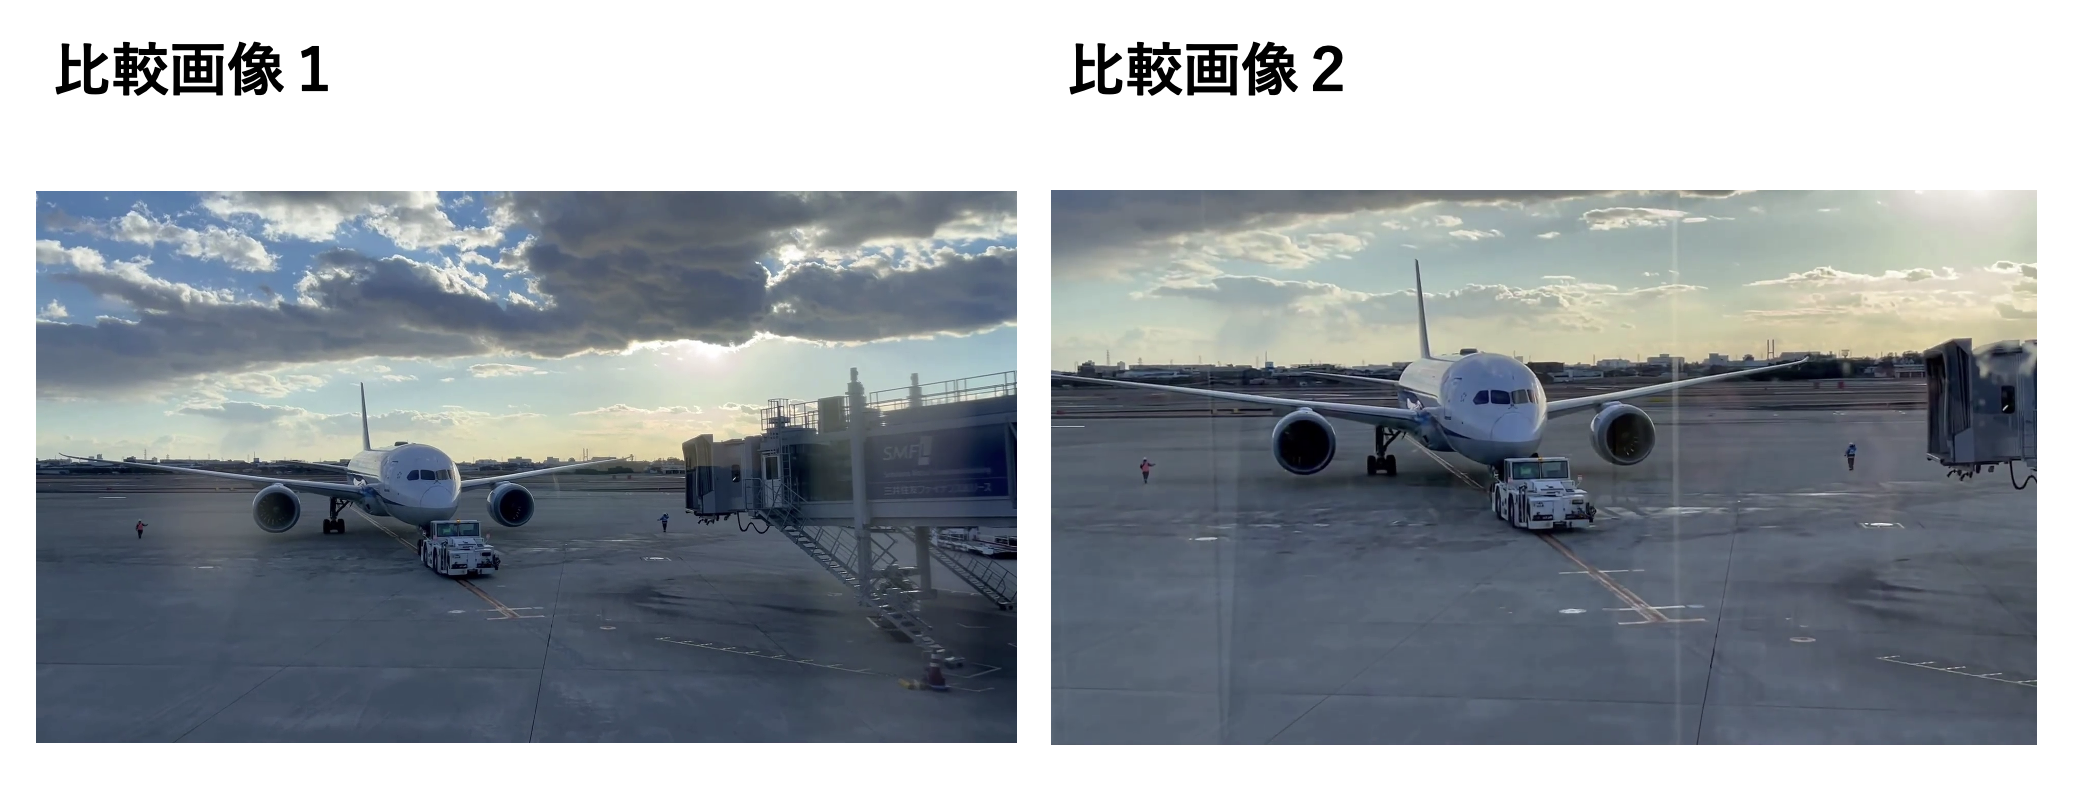
\includegraphics[width=14cm]{image/hikaku.png}}
  \caption{\label{fig:hikaku} 比較サンプル画像}
\end{figure}

\clearpage
\section{研究目的}
従来,個人がデータとして所持している動画データの管理方法は,動画のタイトルや長さ,重さ,撮影時間などであった.
ここに,サードパーティー製のソフトウェアを使用することによって,クラウド上で動画内に何が写っているかの分析が可能となり,より動画の管理が容易になった.

しかし,画像と動画では同じ分析結果を使用できるわけではない.
画像では何が映っているかがわかるとおおよそ画像の整理や検索を行うことができるが,動画では何が写っているかの情報に,時系列情報が付加されている.

本研究では,従来のシステムでは動画に対して時系列情報が付加されていないことに注目し,動画内の物体検出並びに時系列情報を用いた解析を可能とすることを目的とする.

さらに,画像を入力元として扱える動画検索機能を作成することも目的とする.
この機能を実装することにより,これまで動画のワンシーンを「動画のタイトル・ファイル名」と「時間・再生位置」などで管理していたところを,該当するシーンの「スクリーンショット」や「類似している別の画像」を使用することで,対象となる動画および時間を推定することが可能となる.
これによって人力では非常に困難とされている大量の動画データからの検索がより身近なものになると考えられる.

\clearpage

\section{本論文の構成}
以下に本論文の構成を示す.
\begin{description}
\item[第\ref{sec:introducion}章 \qquad 序論]\mbox{}\\
本システムのが概要を示す.

\item[第\ref{sec:algorithm}章 \qquad 画像処理アルゴリズムについて]\mbox{}\\
本システムを開発するにあたって参考にした画像処理アルゴリズムについて述べる.

\item[第\ref{sec:system}章 \qquad 動画解析システムについて]\mbox{}\\
本システムの全体の仕組みや,使用した技術について述べる.

\item[第\ref{sec:consideration}章 \qquad 動作検証と考察]\mbox{}\\
動作結果とともに,本システムの課題や今後の展望について述べる.

\item[第\ref{sec:conclusion}章 \qquad 結論]\mbox{}\\
本システムの開発にあたっての目的と,その達成度について述べる.

\item[付録 \qquad 使用方法]\mbox{}\\
本システムの使用方法について述べる.
\end{description}

\clearpage

\chapter{画像処理アルゴリズムについて}
\label{sec:algorithm}

\section{はじめに}
本章では,本研究を行うにあたり必要な画像処理アルゴリズムと,その基本となる学習処理について述べる.

\section{ニューラルネットワーク}
ニューラルネットワーク (Artificial Neural Network; ANN) とは.人工知能における学習アルゴリズムの一種で.生物学的な神経細胞を模倣して構築された数学的なモデルのことである.
ニューラルネットワークは,人工ニューロンと呼ばれるユニットを組み合わせて構成される.

\subsection{人工ニューロン}
人工ニューロンとは,生物学的な神経細胞を模倣して構築された数学的なモデルである.

人工ニューロンの構成を図\ref{fig:neuron}に示す.

\begin{figure}[b]
  \centering
  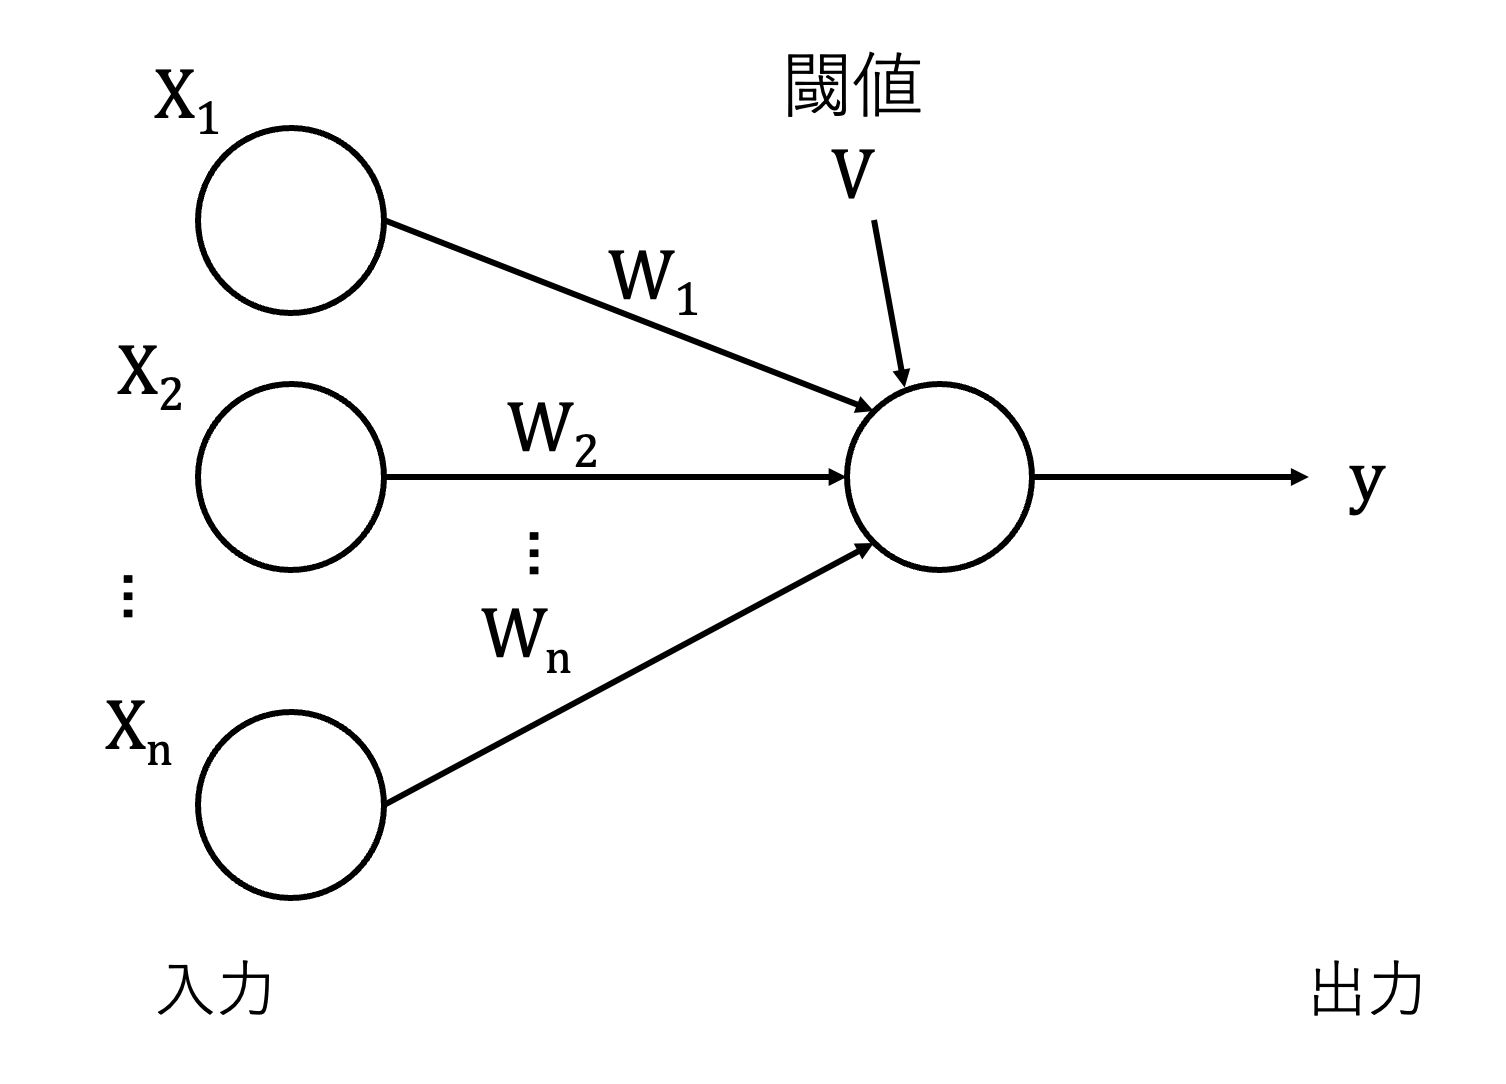
\includegraphics[width=7cm]{image/neuron.png}
  \caption{人工ニューロン}
  \label{fig:neuron}
\end{figure}

人工ニューロンは,外部から与えられたデータやネットワークを構成する他の人工ニューロンから複数の入力を受け取り,適当な計算を施して出力信号を出力する.
図\ref{fig:neuron}より,入力された値$x_i$は,入力ごとに重みと呼ばれる定数$w_i$を掛け合わせる.
入力信号は重みを掛け合わせた上で足し合わせ,しきい値と呼ばれる定数$v$を減算する.
こうして計算を行った積算値$u$を,伝達関数(transfer function)で処理した結果$f(u)$を人工ニューロンの出力$y$とする.
以上の過程を次の(\ref{eq:sum1})式で表現する.


\begin{eqnarray}
  \label{eq:sum1}
  u = \sum_{i=0}^n x_i w_i - v \nonumber \\
  y = f(u)
\end{eqnarray}

伝達関数にはステップ関数(step function)やシグモイド関数(sigmoid function)などがよく用いられる.
ステップ関数は,入力が0以上であれば1を返し,0未満であれば0を返す非線形関数である.
シグモイド関数とは,次の(\ref{eq:frac1})式のような関数である.

\begin{eqnarray}
  \label{eq:frac1}
  f(u) = \frac{1}{1 + \mathrm{e}^{-u}}
\end{eqnarray}

入力$u$が増加すると.出力$f(u)$は1に近づき.入力$x$が減少すると.出力$f(u)$は0に近づく.
つまり.シグモイド関数は入力$u$がどの程度大きいかに応じて.出力$f(u)$がどの程度大きくなるかを制御することが可能となっている.

ただし.シグモイド関数はANNにおいては,勾配消失問題が発生するため,シグモイド関数に代わる別の関数が用いられることが多い.
勾配消失問題については,後述する.

\subsection{ニューラルネットワーク}
ニューラルネットワークの構成図を図\ref{fig:perceptron}に示す.

\begin{figure}[ht]
  \centering
  \fbox{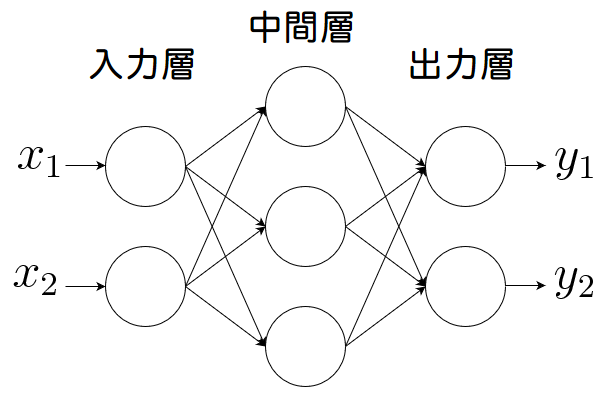
\includegraphics[width=12cm]{image/perceptron.png}}
  \caption{ニューラルネットワークの構成図}
  \label{fig:perceptron}
\end{figure}

入力層は入力信号を次段の人工ニューロンに伝えるだけの固定化した素子である.
入力層から中間層に向かう重みとしきい値は,ランダムに初期化した固定の数値である.
出力層の重みとしきい値は変更可能である.
パーセプトロンは,各階層はいずれも似たような構造であり,階層間の結合も全結合である.


\subsection{学習について}
パーセプトロンの学習は,教師あり学習によって行われる.
教師あり学習とは,教師データと呼ばれる正解データを用いて学習を行う手法である.
教師データには,入力データと正解データが含まれている.
教師データを用いて学習を行うことで,パーセプトロンは入力データに対して正解データを出力するように学習する.

つまり,学習とは,入力された値が正解データと一致するように,パーセプトロンの重みとしきい値を調整することである.

\subsection{誤差逆伝播法}
誤差逆伝播法とは,ニューラルネットワークの学習アルゴリズムの一種で.誤差を伝播させて.各層の重みとしきい値を更新することで.ニューラルネットワークを学習させる手法である.
損失関数 (loss function) と呼ばれる.ニューラルネットワークの予測結果と正解との誤差を最小化することで,より精度の高い結果を得ることができる.

一般的に,逆誤差伝播法は勾配降下法 (Gradient Descent) と組み合わせて使用される.
勾配降下法とは.損失関数を最小化するために重みとバイアスを更新するためのアルゴリズムである.

出力から入力に逆伝播していく際に,伝播関数の部分を微分する必要がある.
活性化関数にシグモイド関数を用いた場合,逆伝播を繰り返すと,微分の結果が0に近づいてしまうという問題がある.
このことを勾配消失問題と呼ぶ.

シグモイド関数と,それを微分した関数を図\ref{fig:sigmoid}に示す.

\begin{figure}[b]
  \centering
  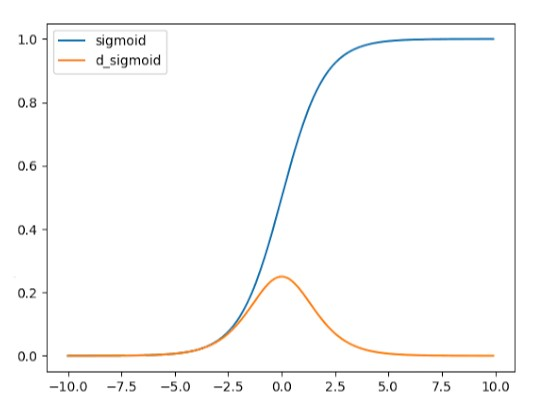
\includegraphics[width=10cm]{image/sigmoid.jpg}
  \caption{シグモイド関数と微分した関数}
  \label{fig:sigmoid}
\end{figure}

微分後の関数の最大値が0.25となるため,隠れ層を繰り返すごとに伝播していく誤差が小さくなってしまう.
そうなると,入力層まで遡った時のフィードバックする値が0に近い値となり,学習が行えなくなってしまう.

この問題を解決するために,活性化関数にはReLU関数やLeaky ReLU関数などが用いられるが多い.

ReLU関数(Rectified Linear Unit)は,入力が0より大きければそのまま出力し,0以下であれば0を出力する関数である.
ただし,入力値が0以下の場合,勾配が0になってしまうため,微分した関数の最大値が0となってしまう.
この問題を解決するために,Leaky ReLU関数が提案された.
Leaky ReLU関数は,入力が0以下の場合,微小な値を出力する関数である.

ReLU関数とLeaky ReLU関数を図\ref{fig:relu}に示す.
これらの活性化関数を用いることにより,勾配消失問題を解決することができ,より深い階層のニューラルネットワークを構築することが可能となる.

\begin{figure}[t]
  \centering
  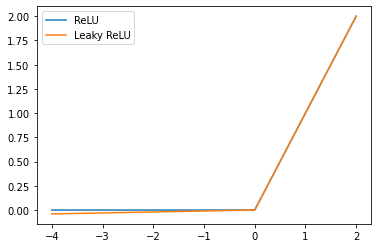
\includegraphics[width=10cm]{image/relu.png}
  \caption{ReLU関数とLeaky ReLU関数}
  \label{fig:relu}
\end{figure}

\section{ディープラーニング(深層学習)}
ディープラーニングとは,人間が行う作業をコンピュータに学習させる機械学習の一種である.
人間の神経をモデルとしたニューラルネットワークを多層化し,コンピュータ自身が大量のデータから特徴を抽出し,予測や分類を行う手法のことである.
ディープラーニングは,ディープニューラルネットワークとも呼ばれる.

\section{CNN(Convolutional Neural Network)}
CNNとは,畳み込みニューラルネットワークとも呼ばれ,画像などの2次元画像処理に特化した多階層の階層型ニューラルネットワークである\cite{cnn}. 
基本構造を図\ref{fig:cnn}に示す.

\begin{figure}[b]
  \centering
  \fbox{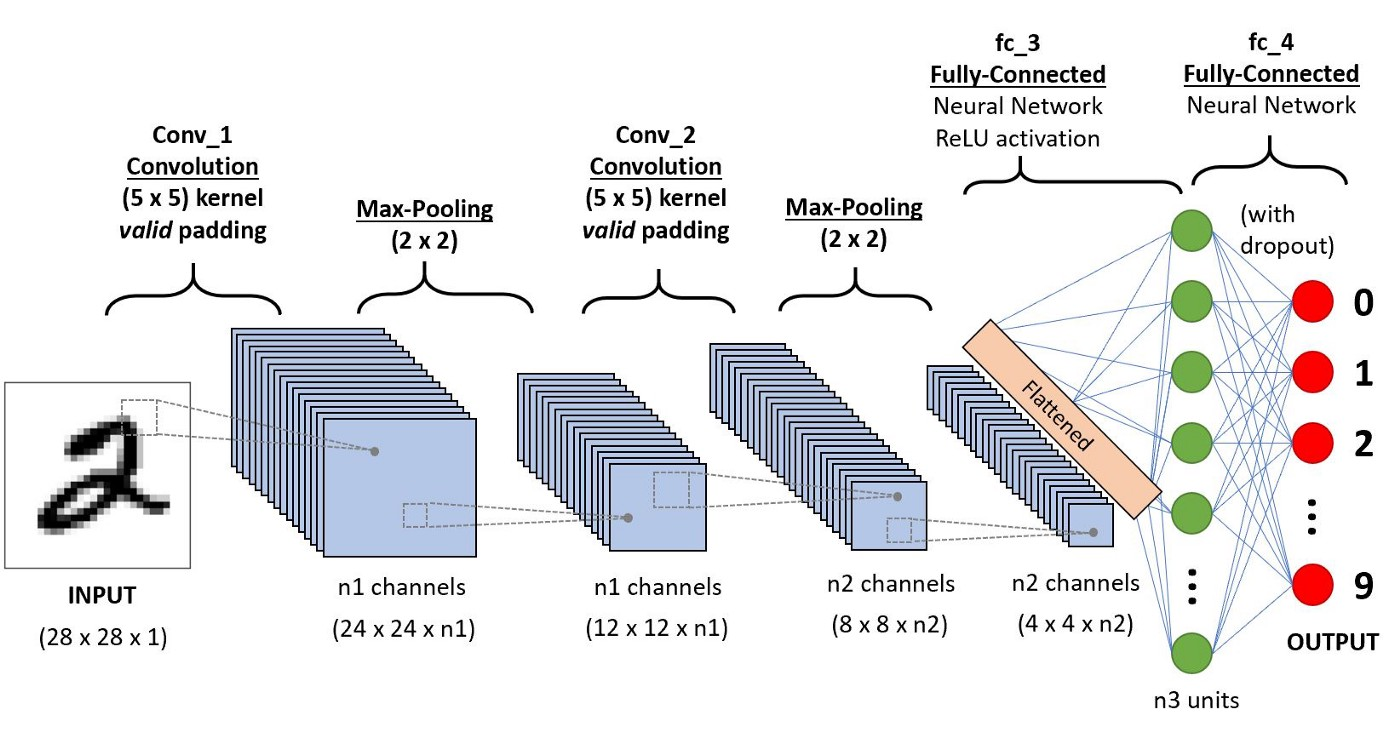
\includegraphics[width=13cm]{image/cnn.jpeg}}
  \caption{CNNの構造}
  \label{fig:cnn}
\end{figure}

パーセプトロンの構造とは違い,CNNには畳み込み層(convolutional layer)と呼ばれる層とプーリング層(pooling layer)と呼ばれる層が存在する.

畳み込み層 (Convolutional Layer)は,カーネルと呼ばれる畳み込みフィルタ (Convolutional Filter) を用いて画像から特徴を抽出する操作のことである.
畳み込みフィルタを複数使用し,畳み込み演算を通して画像の特徴がより強く現れる特徴マップ(Feature Map)を作成する.
この処理では,人間の視覚野が持つ局所受容野に対応しており,移動普遍性の獲得に貢献する.
つまり,畳み込みの処理を通して,「位置のずれ」に強いモデルの作成が可能となる.

プーリング層(Pooling Layer)の役割は,畳み込み層で作られた特徴マップをより小さなものへと変換し,情報の位置ズレに対する頑強さを強めることにある.
そして,maxプーリングと呼ばれる特徴マップの最大値を抽出するものや,aveプーリングと呼ばれる特徴マップの平均値を抽出するものがある.

最後に,全結合層(Fully Connected Layer)で情報を縮約することで,ニューラルネットワークの処理が容易になる.

\clearpage

\chapter{動画解析システムについて}
\label{sec:system}
\section{はじめに}
本章では,本システムの動画解析システムについて説明する.

\section{使用するライブラリについて}
本研究ではFacebook AI Research(FAIR)が公表したDetectron2を使用する.
Detectron2とは,高機能な物体検出およびセグメンテーション機能を有する次世代ライブラリである.\cite{detectron2}
特徴としては,モデルの訓練速度が非常に高速であること,物体の検出数が多いことが挙げられる.
また,一部のプログラム書き換えと使用する学習済みデータの切り替えを行うことで,Classification(画像分類),Object Detection(物体認識)等の豊富な機能を簡単に実装することが可能となっている.

本研究では,動画内に写り込んでいる物体の物体名や位置情報などをデータベースに保存するためにDetectron2のObject Detection機能を使用する.
また,Detectron2で提供されている大規模な学習済みモデルも使用する.
データセットはCOCOモデルで学習したObject Detection向けに配布されているものである.
COCO(Microsoft COCO:Common Objects in Context)とは,画像内の物体の検出やセグメンテーションを行うためのデータセットである.\cite{coco}

使用するデータセットの選択には,物体の検出が多いこと,そして検出時間が短いことが重要である.
Detectron2が公開しているデータセットは表\ref{tab:dataset}の通りである.

\begin{table}[H]
  \centering
  \caption{Detectron2が公開しているデータセット}
  \label{tab:dataset}
  \begin{tabular}{ccccccc}
    \toprule
    \thead{Name} & \thead{lr sched} & \thead{train time(s/iter)} & \thead{inference time(s/im)} & \thead{trainmem(GB)} & \thead{boxAP} \\
    \midrule
    R50-C4 & 1x & 0.551 & 0.102 & 4.8 & 35.7 \\
    R50-DC5 & 1x & 0.380 & 0.068 & 5.0 & 37.3 \\
    R50-FPN & 1x & 0.210 & 0.038 & 3.0 & 37.9 \\
    R50-C4 & 3x & 0.543 & 0.104 & 4.8 & 38.4 \\
    R50-DC5 & 3x & 0.378 & 0.070 & 5.0 & 39.0 \\
    R50-FPN & 3x & 0.209 & 0.038 & 3.0 & 40.2 \\
    R101-C4 & 3x & 0.619 & 0.139 & 5.9 & 41.1 \\
    R101-DC5 & 3x & 0.452 & 0.086 & 6.1 & 40.6 \\
    R101-FPN & 3x & 0.286 & 0.051 & 4.1 & 42.0 \\
    \bottomrule
  \end{tabular}
\end{table}

boxAPとは各モデルの平均精度のことである.
本システムでは,推論時間が短く,精度が高いR50-FPNを使用する.

\section{システム全体の構築と動作について}
本システムの処理の流れを\ref{fig:flow}に示す.

Making Indexでは,動画のインデックス作成およびデータベースへの保存を行う.
ユーザーがアップロードした動画に対し,Detectron2を用いて動画の各フレームに対して解析を行い,その結果をデータベースへ保存する.
この処理を,画像を用いた検索の前にあらかじめ行うことで,画像を用いた検索結果がデータベースを介して高速に行えるようになる.

Search Videosでは,検索として入力した画像と一致や類似する動画のタイムスタンプを,データベースから検索する機能である.
ユーザがアップロードした画像に対して,動画解析時同様にDetectron2を用いた解析を行う.

本システムの解析にはDetectron2を用いるが,解析に使用するデータを全て統一することで,同じ画像を複数回入力しても出力が全て一致する性質を利用する.

システムの全体には,Python製WebフレームワークFlutterを使用する.
画像解析時のPythonコードとシームレスな動作が可能な点,GUIライブラリを使用しなくても良い点などがFlutterを採用した理由である.

データベースについては,次節で詳細に解説する.

\begin{figure}[H]
  \centering
  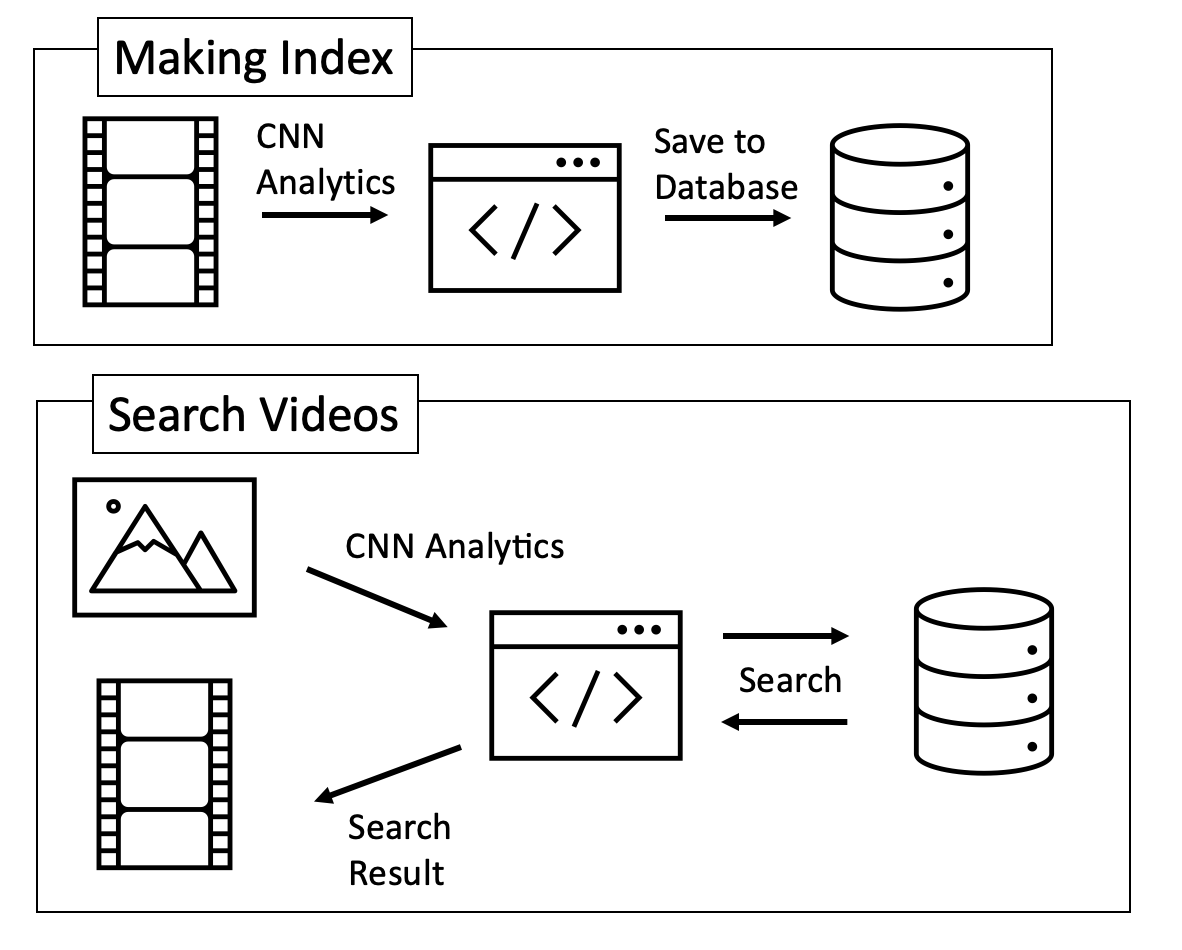
\includegraphics[width=13cm]{image/flow.png}
  \caption{システム全体の流れ}
  \label{fig:flow}
\end{figure}

\subsection{データベースの作成について}
本システムでは,ユーザ情報並びに動画,画像などの情報を,データベースを用いて管理している.
構築しているデータベースは図\ref{fig:table_list}のとおりである.

\begin{figure}[H]
  \centering
  \fbox{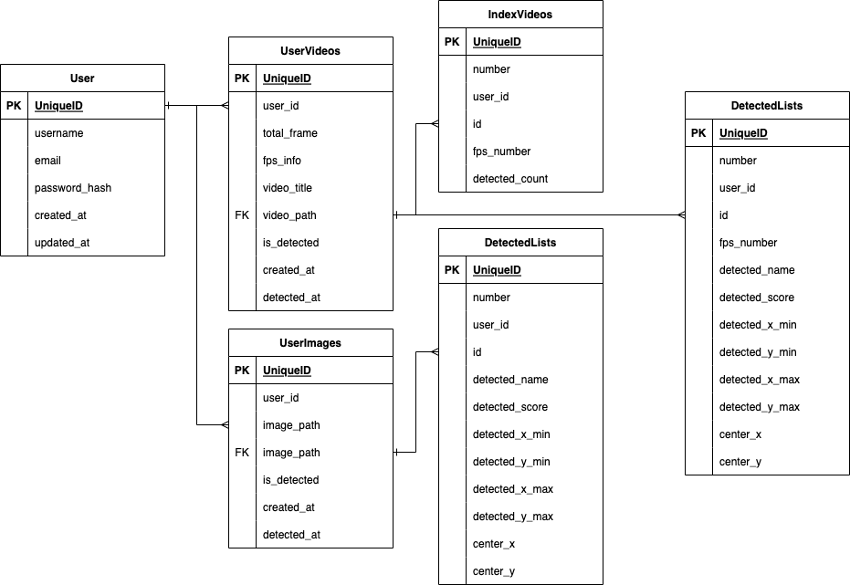
\includegraphics[width=13cm]{image/table_list.png}}
  \caption{データベース図}
  \label{fig:table_list}
\end{figure}

画像検索を利用するには,動画の検索対象となるデータベースを作成するために,動画解析を行う必要がある.
ユーザーがシステムに動画をアップロードすると,自動的に動画解析が開始されるよう実装した.

まず,アップロードされた動画の全フレームにCNNを用いた推論を実施する.
CNNはDetectron2を用いることで一般的な物体に対して推論が可能となる.
その推論データをデータベースに格納する.保存する情報は表\ref{tab:table_list}のようになっている.

\begin{table}[H]
  \centering
  \caption{DetectedListsテーブルの詳細}
  \label{tab:table_list}
  \begin{tabular}{cc}
    \toprule
    \thead{detected lists} & \thead{説明} \\ 
    \midrule
    number & 固有のID \\
    id & ユーザID \\
    fps number & 動画のフレーム番号 \\
    detected name & 検出されたオブジェクトの物体名 \\
    detected score & 検出されたオブジェクトの認識率 \\
    detected x_{min} & 検出されたオブジェクトのx座標の最小値 \\
    detected y_{min} & 検出されたオブジェクトのy座標の最小値 \\
    detected x_{max} & 検出されたオブジェクトのx座標の最大値 \\
    detected y_{max} & 検出されたオブジェクトのy座標の最大値 \\
    center x & 検出したオブジェクトの中心のx座標\\
    center y & 検出したオブジェクトの中心のy座標 \\
    \bottomrule
  \end{tabular}
\end{table}

\subsection{データベースの利用について}
ユーザーがアップロードした動画の中で,自動で解析が完了したものについてはデータベースを用いた検索機能が利用できる.

ユーザーが画像をシステムにアップロードすると,動画のアップロード時同様自動で解析される.
画像に対してCNN(Detectron2)を用いた推論を行い,得られた情報をデータベースに保存する.
そして事前にデータベースに保存しておいた動画の解析データと画像の解析データを用いた検索を開始する.
検索方法は大きく2つに分けられ,次節で詳しく説明する.

\section{オブジェクトの位置情報を用いた検索システムについて}
動画の解析データと画像の解析データを比較してオブジェクトの位置情報を用いた類似シーンを検索する手法について説明する.

処理の手順は下記のようになる.
\begin{enumerate}
  \item 入力した画像のオブジェクト検出リストをデータベースから取得
  \item 検索対象となっている動画の各フレームで検出したオブジェクト検出リストをデータベースから取得
  \item 画像と動画のリストが一致しているか確認する
\end{enumerate}

実装する上で注意すべき点がいくつかある.

まず,動画と画像のx,y座標を実際の値を使用するのではなく,プロットの位置座標を画像のサイズで割った値を使用するという点である.
x,y座標で実際の値を使用した例を図\ref{fig:compare}に記載する.

\begin{figure}[H]
  \centering
  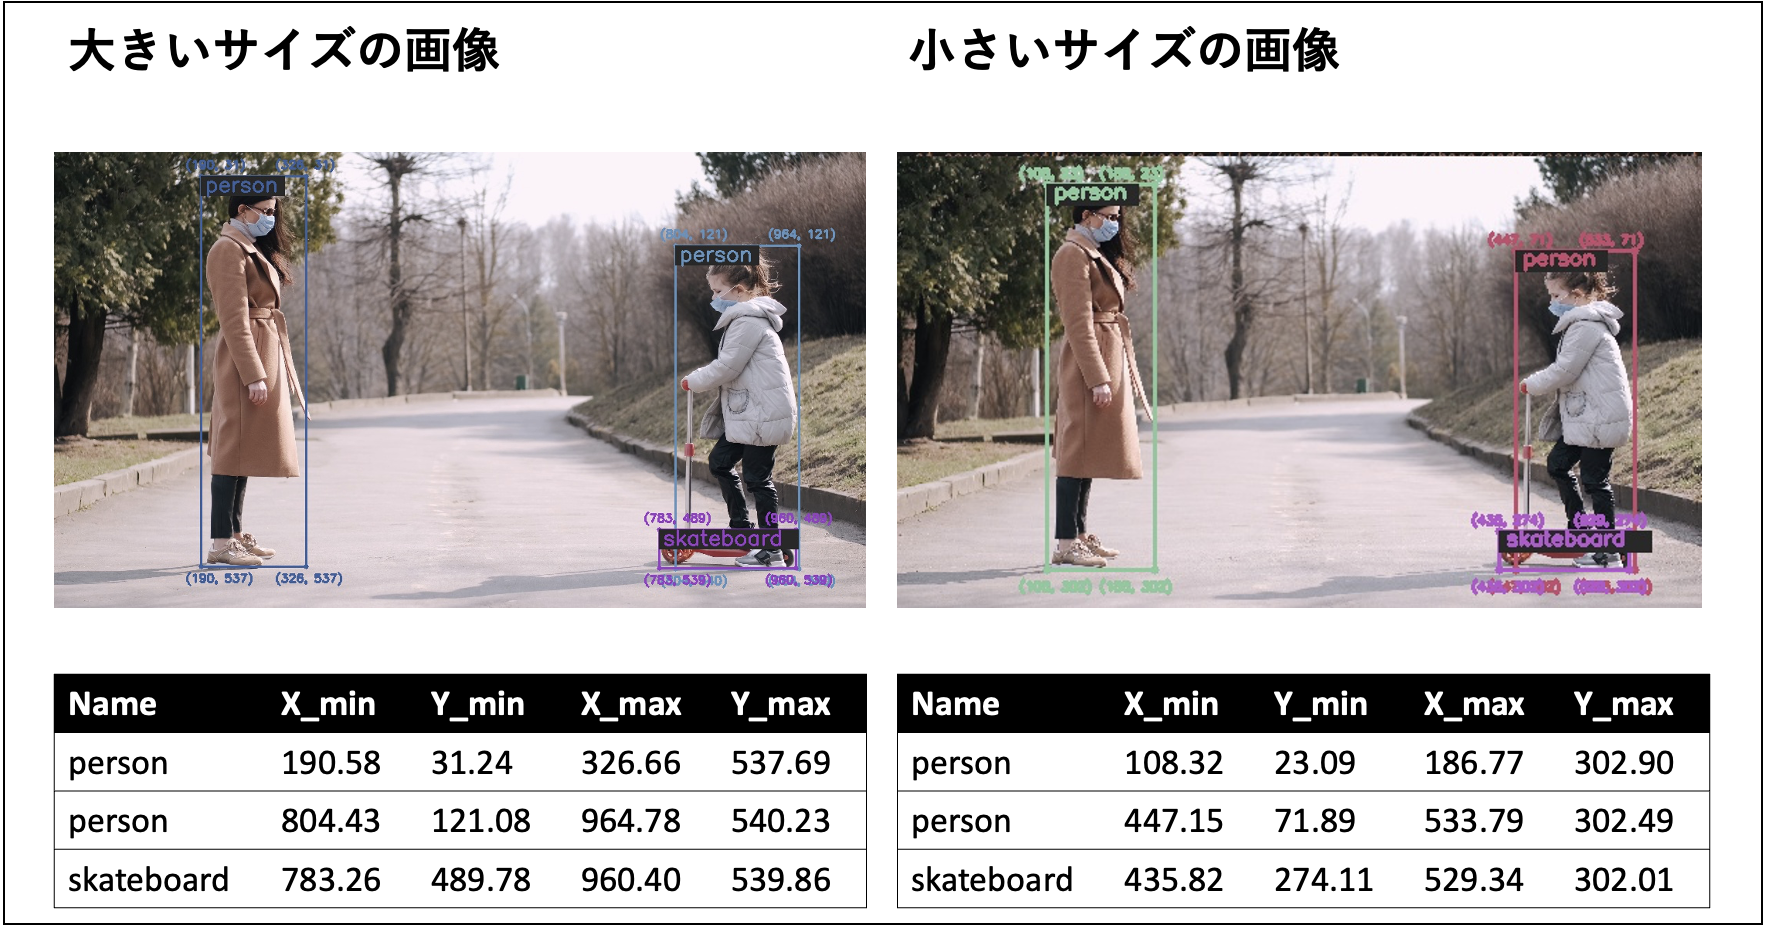
\includegraphics[width=13cm]{image/compare.png}
  \caption{サイズの異なる画像の比較図}
  \label{fig:compare}
\end{figure}

このように一見同じ位置に存在しているように見えるものでも,画像のサイズによってデータベース上の位置情報が異なることがわかる.
このデータをサイズで割ることで実質的に画像の位置情報を正規化することができ,比較しやすい値になる.

また,Detectron2が複数のオブジェクトを検出する際に,出力の手順が一定でないことがある.
同じ画像を入力した際の出力は全く同じ出力がなされる.
しかし,少しでもオブジェクトの位置がずれた別の画像が入力された際の出力は,オブジェクトの検出が異なるため,手順3のリスト比較が容易ではなくなる.
そのため,リストを比較する際にソート等を行なって,リストを整理してから比較した方が処理が簡単になる.
今回のシステムでは,オブジェクト名でソートし,さらにその中でオブジェクトの座標のX座標の昇順,Y座標の昇順でソートしている.
これにより,Detectron2から出力される順番が揃っていないリスト同士も比較が可能となっている.



\section{オブジェクトの位置関係を用いた検索システムについて}
動画の解析データと画像の解析データのオブジェクト間の位置関係を用いた類似シーンの検索について説明する.
位置関係が類似しているデータとは,各オブジェクト間の距離と角度を用いることで検出できると考えられる.
具体的には,次の図\ref{fig:object_relationship}を参照したい.

\begin{figure}[b]
  \centering
  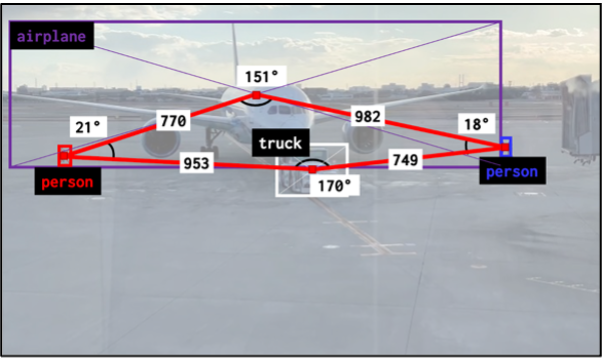
\includegraphics[width=13cm]{image/object_relationship.png}
  \caption{検索結果}
  \label{fig:object_relationship}
\end{figure}

これらのデータを用いることで類似度の算出が可能となる.
この図では,画像から検出したオブジェクトの位置関係を示している.
位置関係を画像と動画で類似度を計算し,類似シーンの算出が可能となる.

ここで,評価関数に入力される物体の検出リストと,結果として扱われる出力について解説する.
まず,入力するデータは次のとおりである.

\begin{eqnarray}
  \label{eq:object_list}
<<<<<<< HEAD
  [[\text{“オブジェクト名“},x_{min},y_{min},x_{max},y_{max},\text{UUID}],\cdots]
=======
  [[‘オブジェクト名’,x_{min},y_{min},x_{max},y_{max}],……]
>>>>>>> parent of 36117c4 (考察増やした)
\end{eqnarray}

このようなPythonのリスト構造で動画と画像の物体名と座標が与えられる.
ここでのx_{min}とは,表\ref{tab:table_list}のものと同じである.

このとき,Detectron2の検出した順番でリストが作成されるため,動画の物体検出リストと画像の物体検出リストを比較する際に何かしらの基準でソートする必要がある.

そこで,リストのソートを行う基準を作成する.
すべてのオブジェクト同士の距離と角度を計算し,角度が一番小さいオブジェクトを次の基準のオブジェクトとする.
すべてのオブジェクトが基準となるまで計算を繰り返し,その基準となったオブジェクトがソートされたリストとなる.
この処理を行うことで,この図のような様々なリストが与えられた場合でも,リストのソートが可能となる.
ただし,このリストは2つのリストの開始位置がずれているため,その部分の修正も行う必要がある.
例えば,図\ref{eq:object_list_before_sort}のリストの場合,オブジェクト名だけに注目したリストを作成すると次のようになる.

\begin{eqnarray}
<<<<<<< HEAD
  \label{eq:center_x}
  x_{center} = \frac{x_{min}+x_{max}}{2}
\end{eqnarray}
\begin{eqnarray}
  \label{eq:center_y}
  y_{center} = \frac{y_{min}+y_{max}}{2}
=======
  \label{eq:object_list_before_sort}
  画像のリスト = [[‘person’, …], [‘person’, …], [‘skateboard’, …]] \\
  動画のリスト = [[‘person’, …], [‘skateboard’, …], [‘person’, …]]
>>>>>>> parent of 36117c4 (考察増やした)
\end{eqnarray}

このリストは並び方が同じであるものの,リストの開始位置が合っていないため,データの比較が難しい.
そこで,画像のリストの先頭のデータを取り出し,最後に追加すると,次のようになり,比較しやすりリスト同士となる.

\begin{eqnarray}
  \label{eq:object_list_after_sort}
  画像のリスト = [[‘person’, …], [‘skateboard’, …], [‘person’, …]]\\
  動画のリスト = [[‘person’, …], [‘skateboard’, …], [‘person’, …]]
\end{eqnarray}

この方法でリストの並び替えを行なっていくが,並び替えが一周しても画像と動画のリストが一致しない場合は,検出したオブジェクト自体が異なっていることとなるため,このフレームでの比較はこれ以上行われず次のフレームの比較が行われる.

<<<<<<< HEAD
繰り返す処理が完了すると,全てのオブジェクトの外周を直線で結ぶ図形を図\ref{fig:figure_2}のように作成することができる.
=======
次に動画と画像で出力されたソート済みのリスト同士の比較を行う.
ここで比較することは,オブジェクト間の距離,角度である.
距離については,すべての辺に対して比を計算し,動画と画像での比がどの程度一致しているかを計算する.ま
た,角度については,同じオブジェクト間の角度についてどの程度一致しているかを計算する.
>>>>>>> parent of 36117c4 (考察増やした)

どの程度ずれているかは,辺の比と角度の分散を参考にした.
その値が大きいとデータにばらつきがあるという認識ができ,図形が一致していないと評価する.

<<<<<<< HEAD
また,(\ref{eq:object_list})式のリストの順番は,図形の最短経路で結んだ順番になっている.

次に,オブジェクト間の距離と図形の内角を計算する.
(\ref{eq:object_list})式の順番が,図形の最短経路で結ぶ順番でソートされているため,図形の内角は,(\ref{eq:angle})式で求めた角度の差分を計算することで求めることができる.
使用する座標は,(\ref{eq:object_list})式から隣り合っている3点を選択し,2つの辺を作成する.
その2つの辺のなす角度を計算することで,図形の内角を求めることができる.
2つの辺は,3つの点をそれぞれ($x_1$, $y_1$), ($x_2$, $y_2$), ($x_3$, $y_3$)とすると,(\ref{eq:edge})式で求める.
\begin{eqnarray}
  \label{eq:edge}
  \vec{e_1} = \left( \begin{array}{c} x_2-x_1 \\ y_2-y_1 \end{array} \right) \\
  \vec{e_2} = \left( \begin{array}{c} x_3-x_1 \\ y_3-y_1 \end{array} \right)
\end{eqnarray}

角度の計算には,(\ref{eq:angle2})式を用いる.
\begin{eqnarray}
  \label{eq:angle2}
  \theta = \arccos \left( \frac{\vec{e_1} \cdot \vec{e_2}}{|\vec{e_1}| |\vec{e_2}|} \right)
\end{eqnarray}

この処理を(\ref{eq:object_list})式のリストの要素全てに対して行うことで,図形の全ての内角を計算することができる.

オブジェクト間の長さについては,(\ref{eq:edge})式で求めた$\vec{e_1}$で求めることができる.


以上の処理を入力された画像および動画の各フレームに対して行うことで,類似シーンの検索を行うことができる.


次に,図形の外周を通る順番でソートされたオブジェクトのリストを用いて,類似シーンの検索を行う.

入力された画像と動画のフレームが類似しているかを判定する基準として,以下の4つを用いる.
\begin{itemize}
  \item オブジェクトの検出数が同じであること
  \item オブジェクトの物体名が同じであること
  \item オブジェクト同士を最短経路で結ぶ図形のそれぞれに対応する辺の比率が同じであること
  \item オブジェクト同士を最短経路で結ぶ図形のそれぞれに対応する内角が同じであること
\end{itemize}

ただし,上記の条件では,オブジェクトの位置関係が100\%一致している必要があるため,類似シーンの検索には基準が厳しいと考えられる.

この類似シーンの検索の結果には,拡大や縮小,回転などの変形が含まれている場合にも,類似性が高いと評価し,結果を出力したい.
そのため,下記の条件を追加する.
\begin{itemize}
  \item オブジェクト同士を最短経路で結ぶ図形のそれぞれに対応する辺の比率が似ていること
  \item オブジェクト同士を最短経路で結ぶ図形のそれぞれに対応する内角が似ていること
\end{itemize}
ここでの具体的な数値については設定せず,それぞれの結果をソートして,上位の結果を出力することで,類似シーンの検索を行う.

図形が少しでも変形すると,辺の比率や内角の大きさが変化するため,図形全体でどの程度ずれているかを最後に計算する.
計算する値は,図形の回転角度,オブジェクト間の長さの比率の平均,オブジェクト間の長さの比率の分散,オブジェクト間の角度の分散である.

オブジェクト間の辺の長さについては,辺の比率の平均を計算する.
この値は,図形の拡大・縮小の度合いを表す.
値が大きくなればなるほど,図形が拡大されていることを示し,値が小さくなればなるほど,図形が縮小されていることを示す.

また,長さの比率の分散を計算する.
オブジェクト間の角度については,角度の分散を計算する.
どちらの値も,この値が大きくなればなるほど,図形が変形されていることを示す.

また,回転した図形についても,類似性が高いと評価したいため,図形の回転角度も考慮する.
なお,回転角度の計算には,オブジェクト同士を最短経路で結ぶ図形のそれぞれに対応する辺同士の角度の平均を用いる.

以上の過程を経て,類似シーンの検索を行う.
結果の出力では,図形の回転角度,オブジェクト間の長さの比率の平均,オブジェクト間の長さの比率の分散,オブジェクト間の角度の分散を出力する.

図形の形が似ている場合の出力結果を最優先したいため,図形のオブジェクト間の角度の分散を基準の出力のソートを行い,結果を出力する.
=======
>>>>>>> parent of 36117c4 (考察増やした)

\section{まとめ}
本システムの動画検索システムの基本的な動作について述べた.

\clearpage

\chapter{考察}
\label{sec:consideration}

\section{システム全体について}
システム全体として安定した動作になっている.

しかし,検索時にかかる時間が無視できないほどにかかってしまう.
本システムでは時間がかかる処理が大きく2つに分かれている.

1つは,動画をアップロードした際に実行される動画解析である.
もう1つは,解析したデータの中から結果を抽出する部分である.

1つ目の解析時間については,GPU・CPUの性能が向上すると解析時間が短くなると考えられる.
また,使用する学習済みモデルを変更・改良することで時間の短縮が見込める.
解析したデータの中から結果を抽出する部分については,様々な複合的な処理が検索結果の表示に時間を要している.
例えば,データベースからデータを抽出する際にSQLを実行しているが,そのトランザクション回数が増えるほど検索の結果表示までに時間を要することになる.
また,オブジェクトが増えるほど,オブジェクト間の位置関係の計算量が増えるため,処理に時間がかかることになる.
これについては,CPUの性能向上の他,プログラム内のデータ転送速度向上でも高速化が見込める.

検索性能については次節で述べる.

\section{位置情報を用いた検索システムについて}
本システムの実際の検索結果をもとに,位置情報を用いた検索システムの精度を考える.
なお,動画内のフレームを全て示すことが難しいため,動画の一定時間ごとに抽出したものを示すことにする.
検証には,検索対象となる動画を4つ用意し,全てアップロード,並びに解析済みである.
動画1つ目は,親子が向かい合っている動画である.図\ref{fig:movie1}を参照したい.
図\ref{fig:movie2}は動画2つ目で,飛行機がプッシュバックしているシーンを撮影した動画である.
3つ目の動画として図\ref{fig:movie3}の時計しか映っていない動画を用意した.
また,オブジェクトが大量に映っている動画も解析を行い,図\ref{fig:movie4}のような4つ目の動画を用意した.

\begin{figure}[H]
  \centering
  \includegraphics[width=13cm]{image/1_result.jpg}
  \caption{動画1つ目}
  \label{fig:movie1}
\end{figure}

\begin{figure}[H]
  \centering
  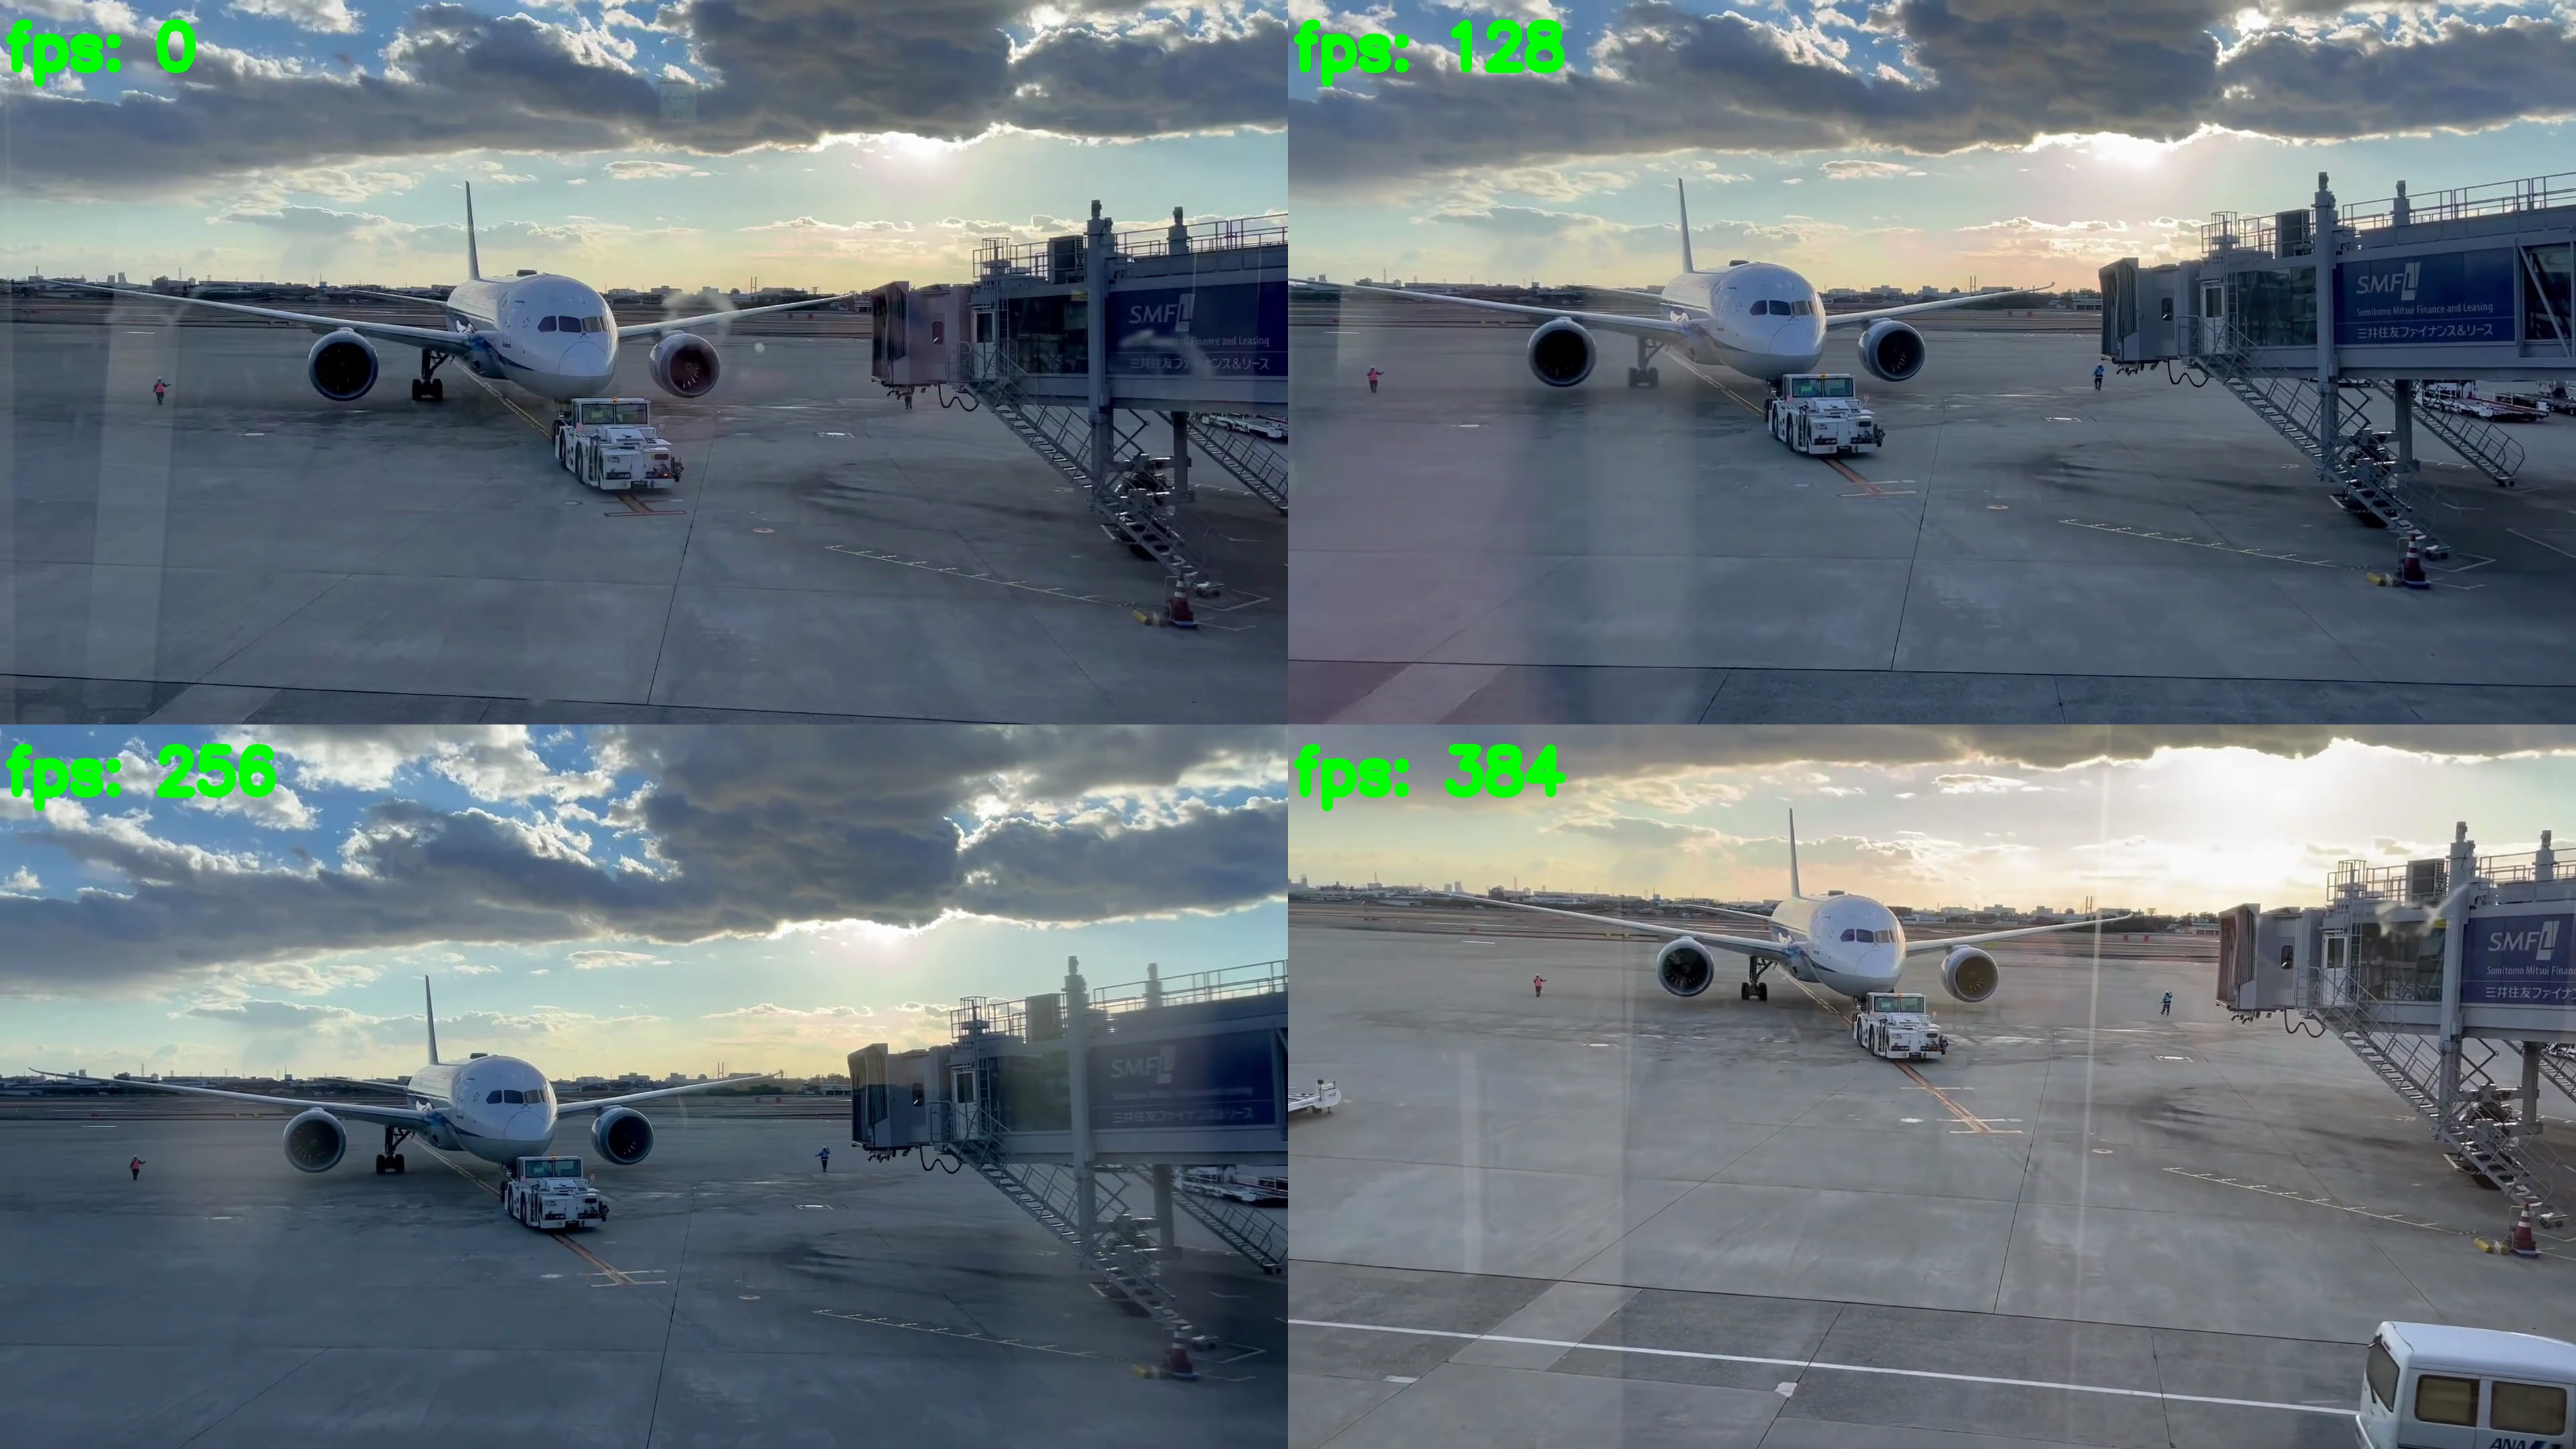
\includegraphics[width=13cm]{image/2_result.jpg}
<<<<<<< HEAD
  \caption{飛行機がプッシュバックしているシーンを撮影した動画}
=======
  \caption{動画2つ目}
>>>>>>> parent of 36117c4 (考察増やした)
  \label{fig:movie2}
\end{figure}

\begin{figure}[H]
  \centering
  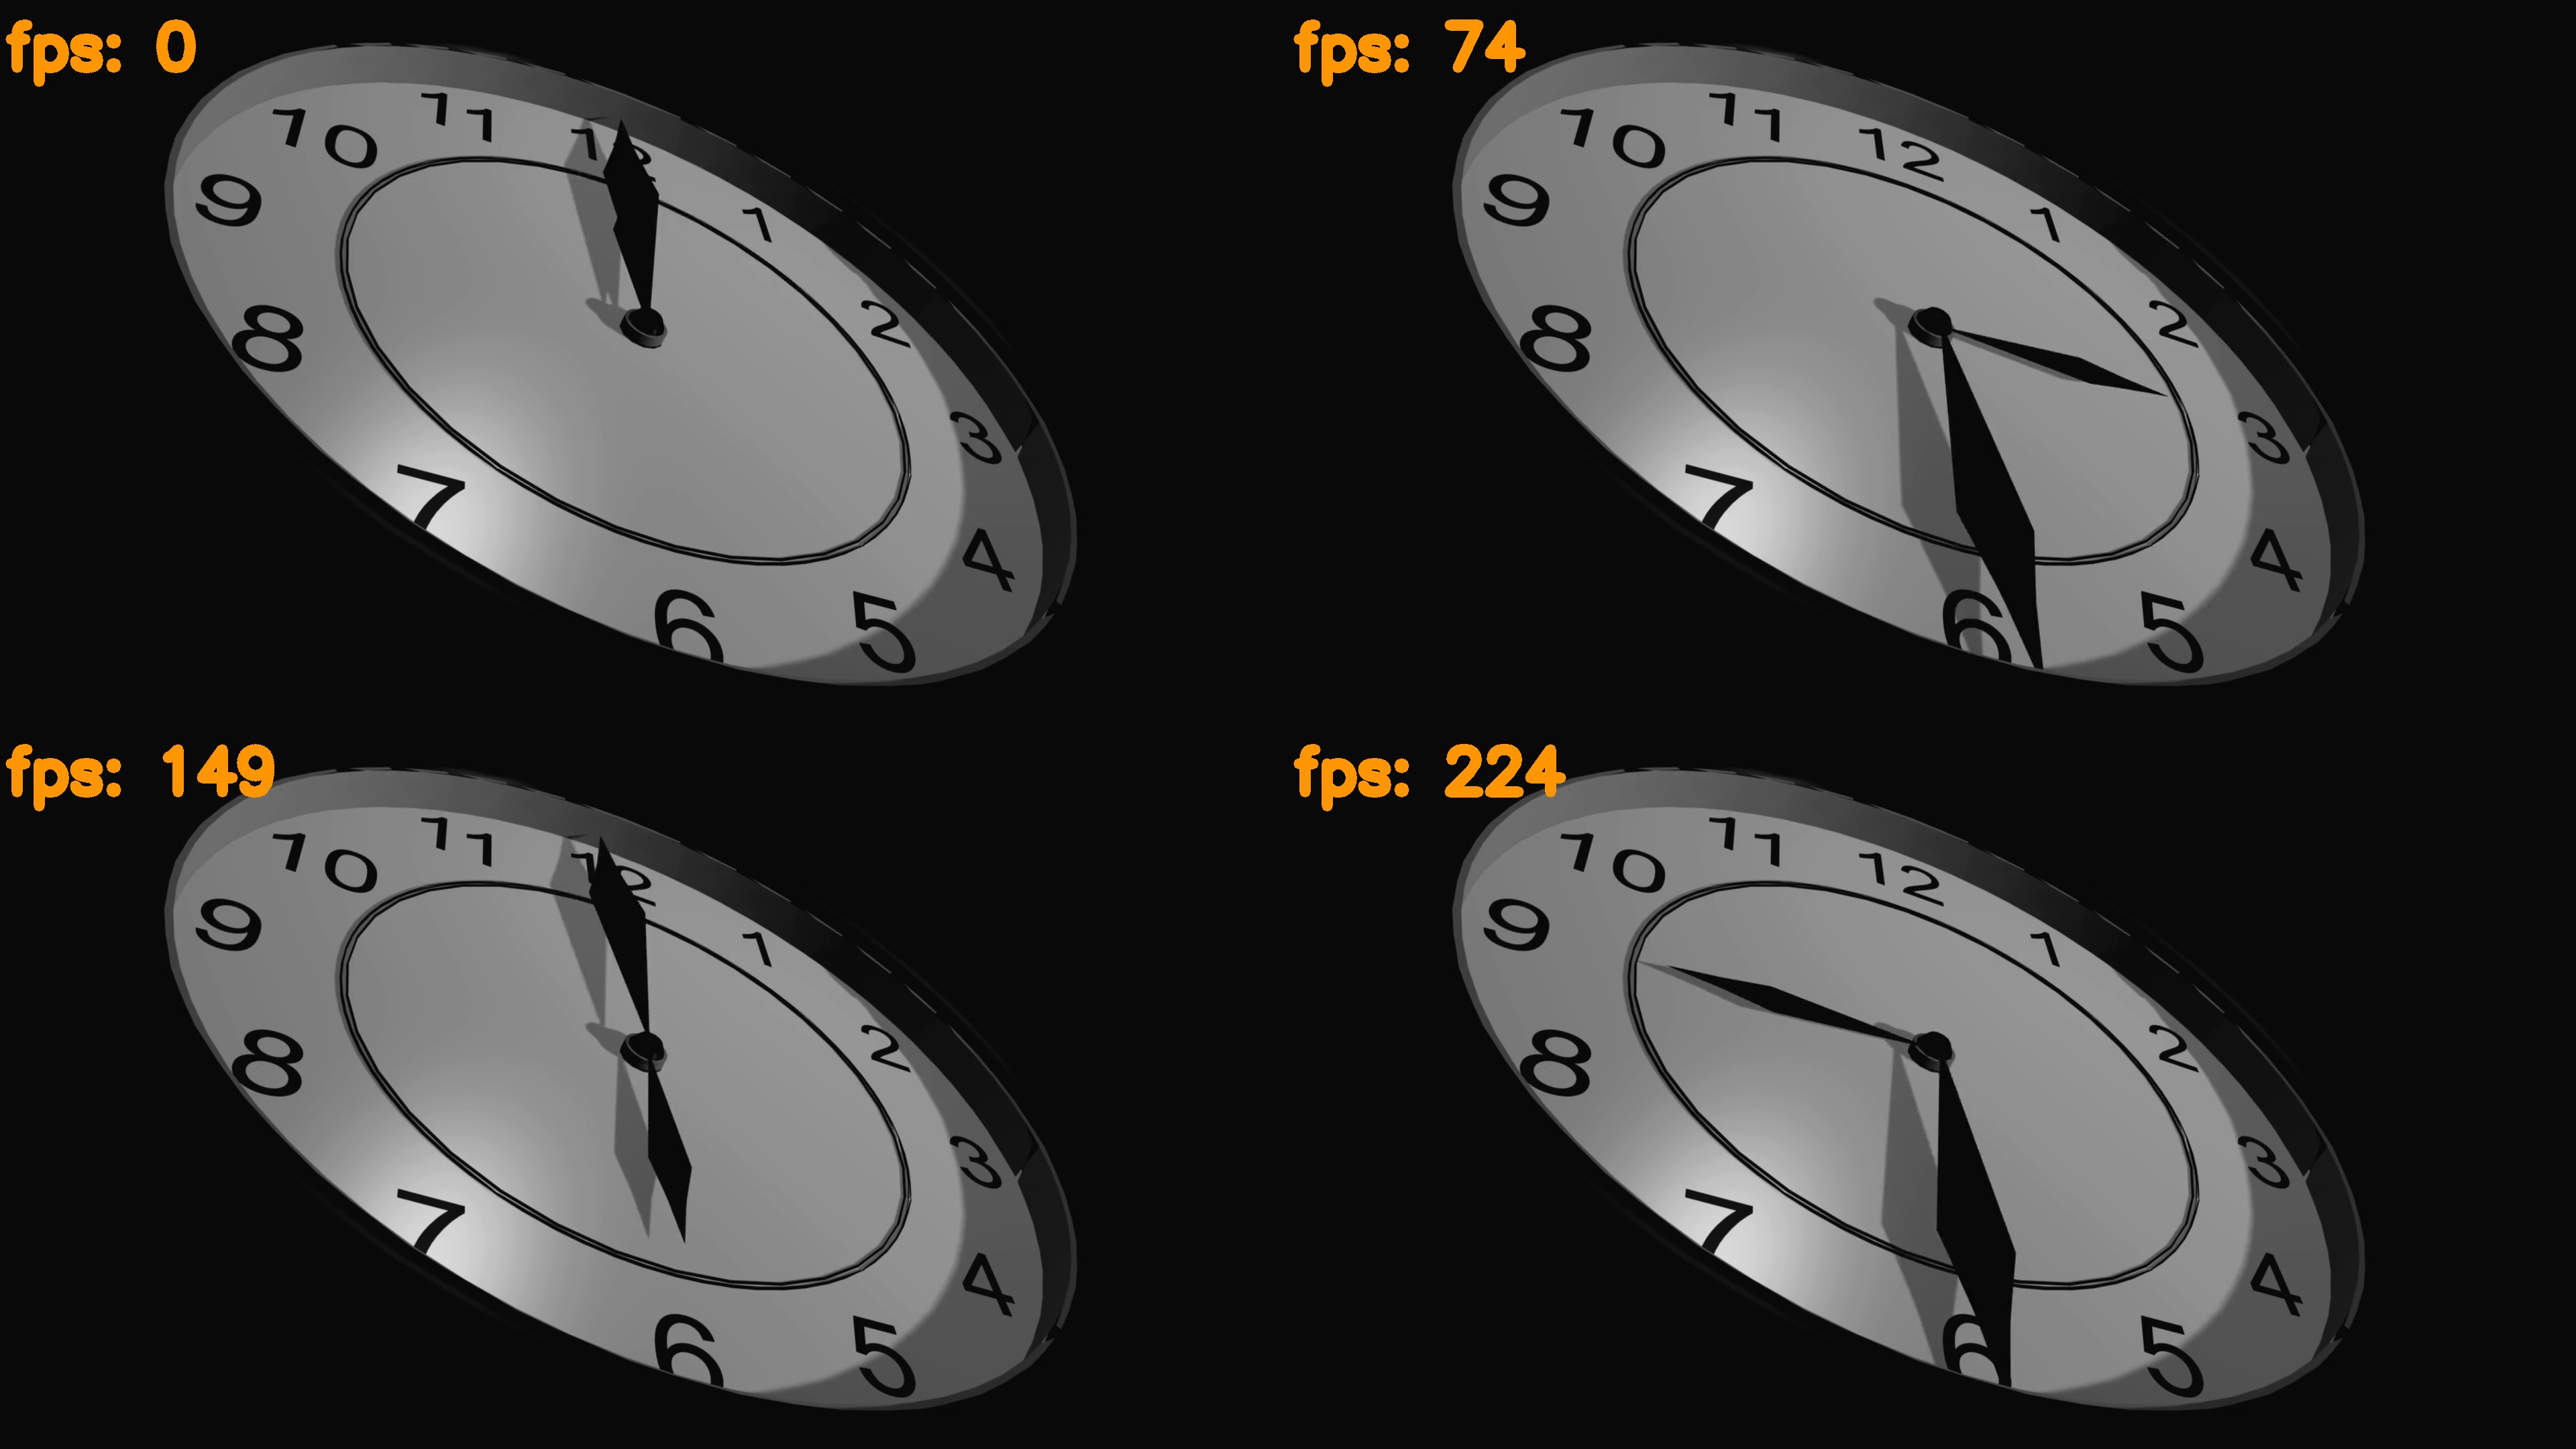
\includegraphics[width=13cm]{image/3_result.jpg}
  \caption{動画3つ目}
  \label{fig:movie3}
\end{figure}

\begin{figure}[H]
  \centering
  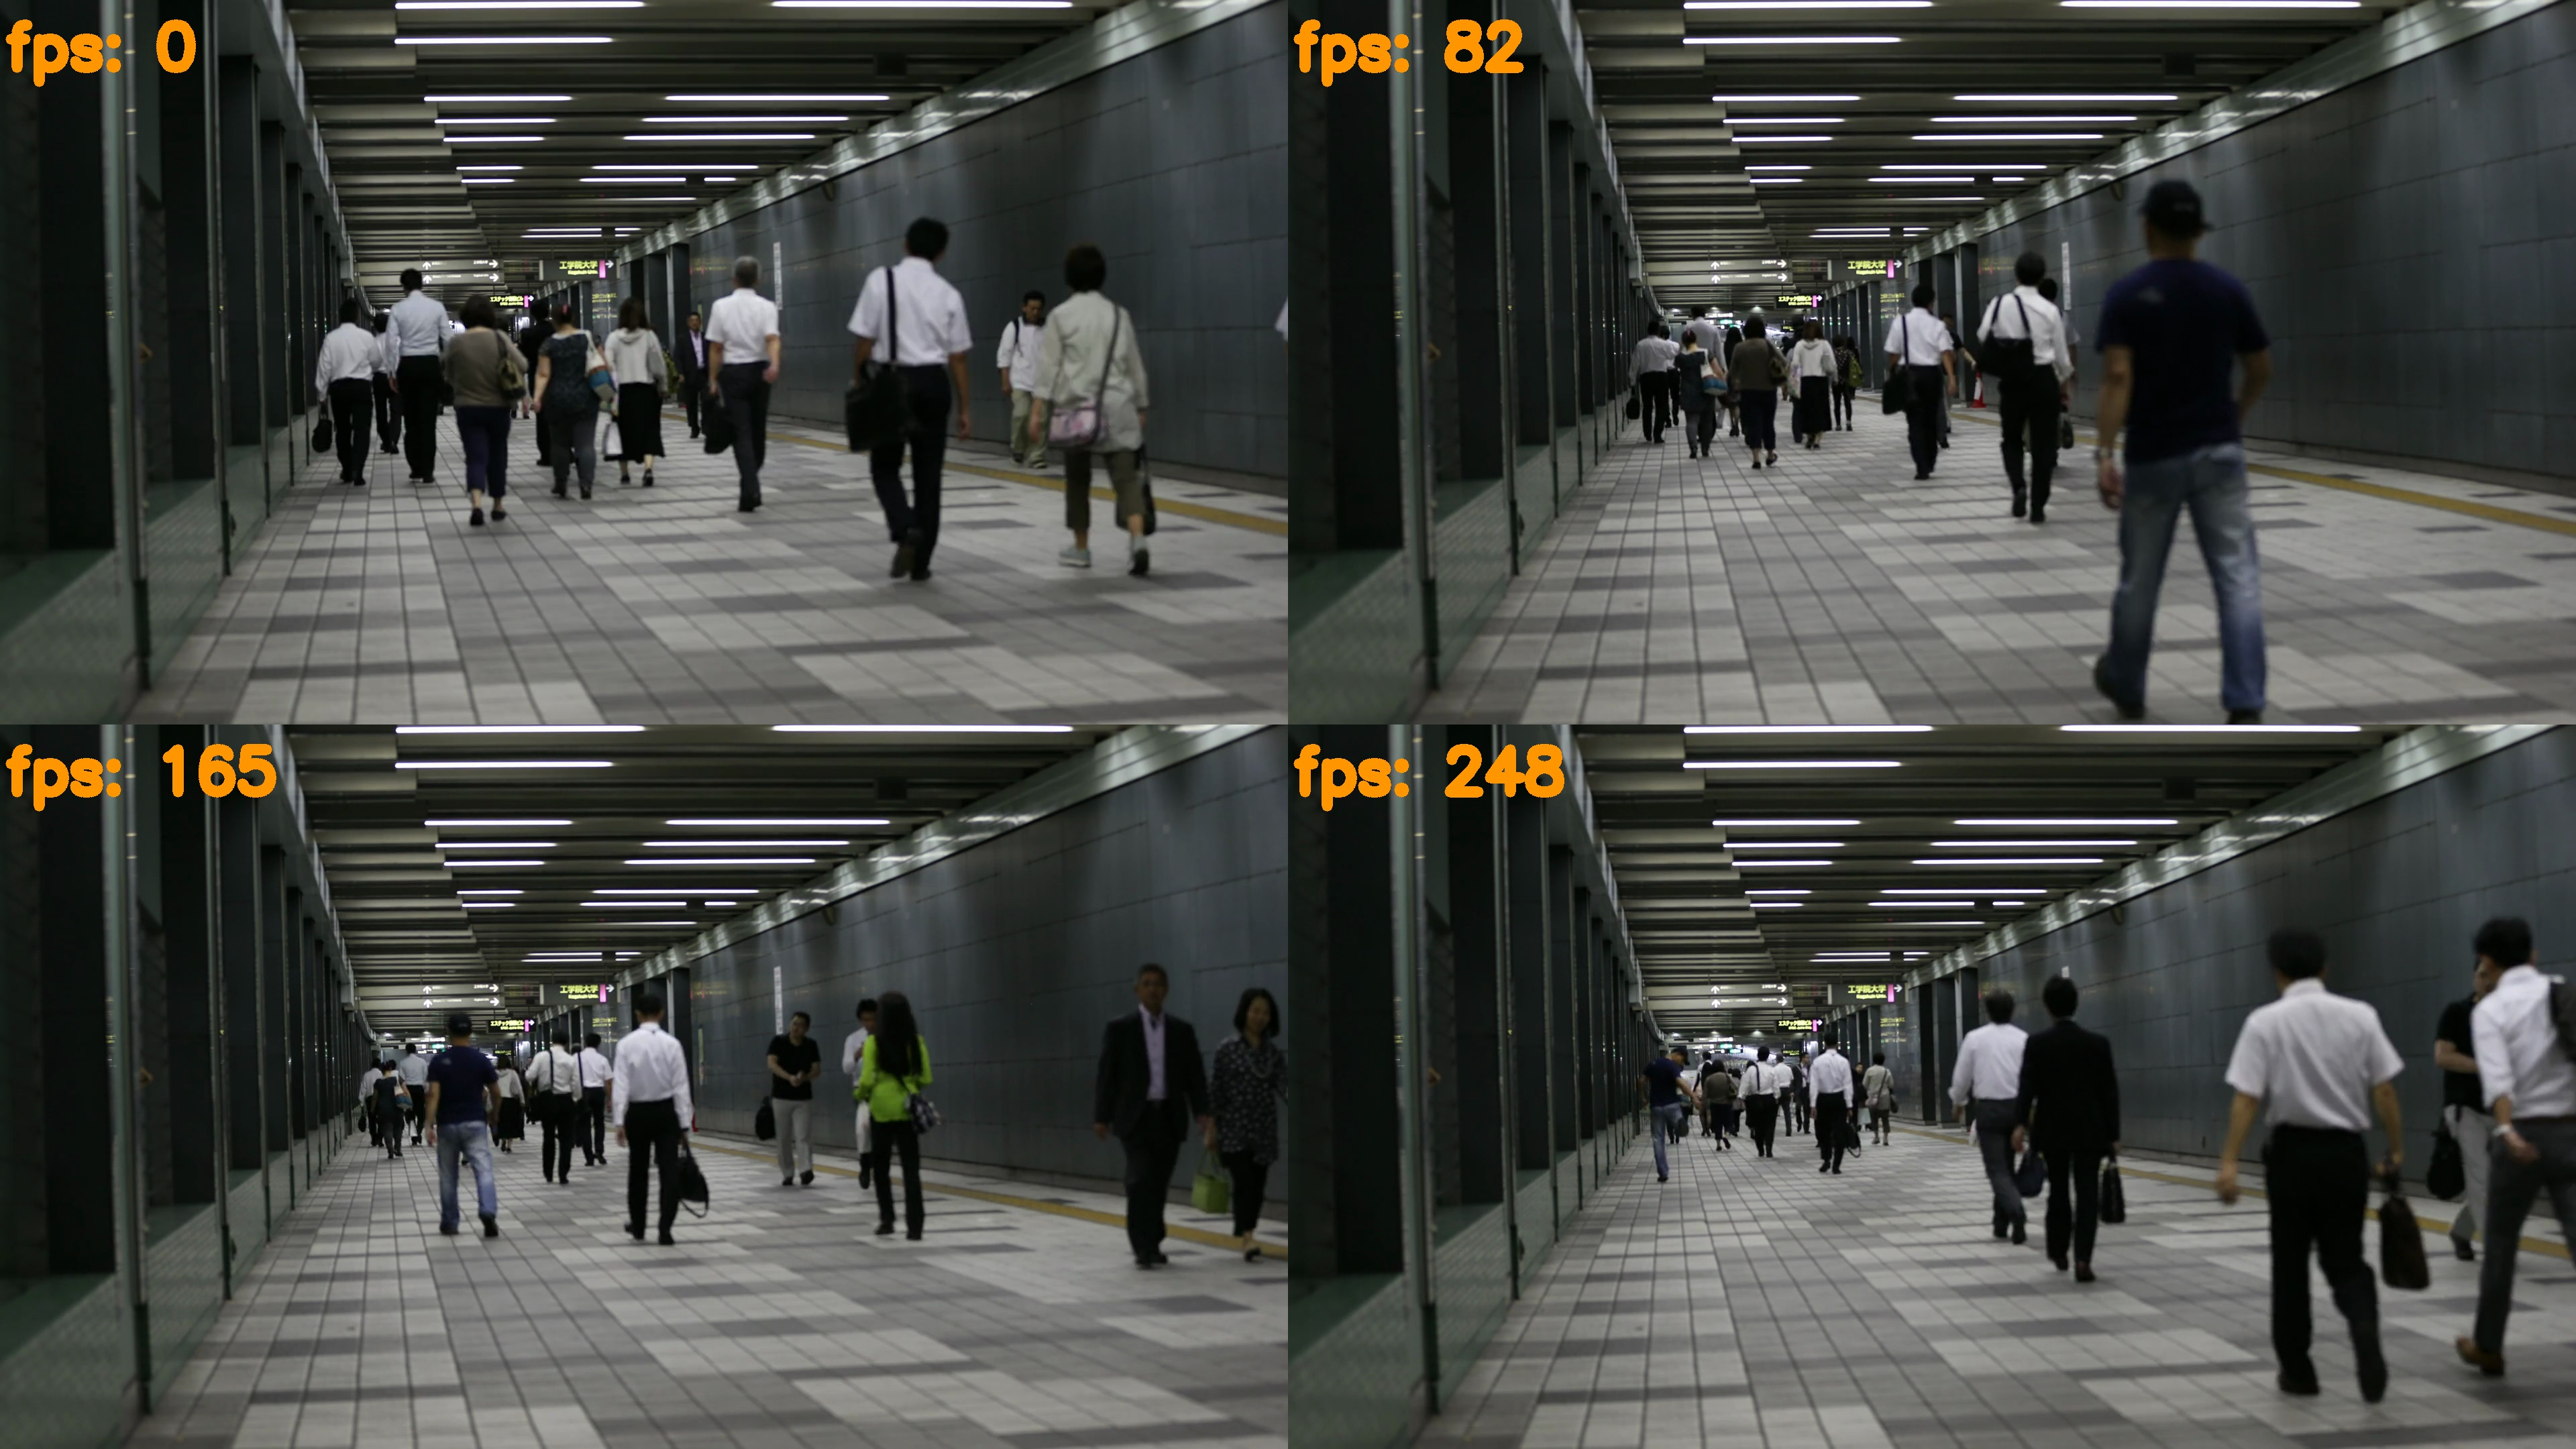
\includegraphics[width=13cm]{image/4_result.jpg}
  \caption{動画4つ目}
  \label{fig:movie4}
\end{figure}

次に入力した画像と結果を示す.図\ref{fig:img_1-1}に示す.
\begin{figure}[b]
  \centering
  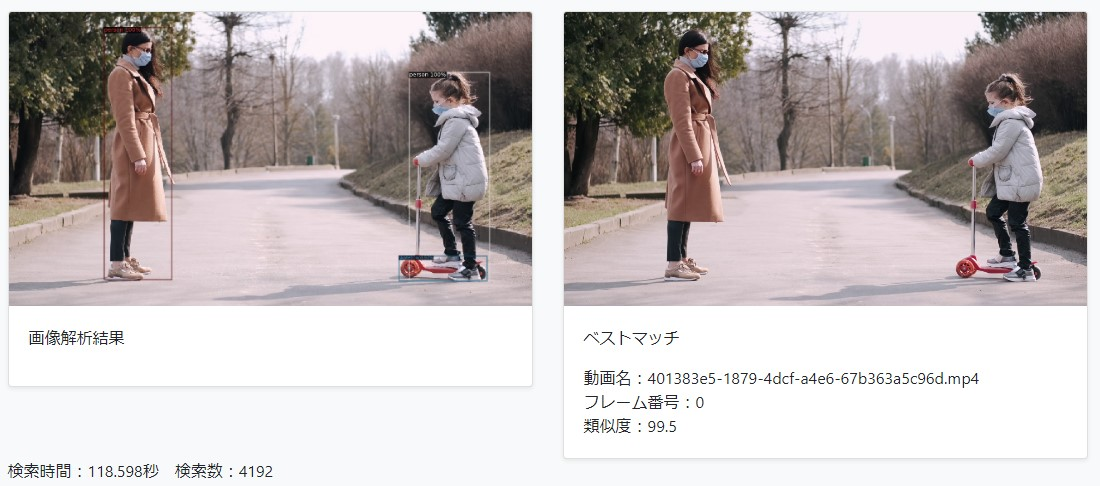
\includegraphics[width=13cm]{image/result_1_1.jpg}
  \caption{検証画像1}
  \label{fig:img_1-1}
\end{figure}

入力した画像と検索結果の動画フレームがほぼ一致していることがわかる.
オブジェクトは,personとskateboardが検出されている.
<<<<<<< HEAD
スコアが一番高いものがベストマッチとして表示されているが,類似シーンがあれば,表\ref{tab:tab_1_1}のように類似度順で出力される.

\begin{table}[t]
  \centering
  \caption{図\ref{fig:img_1_1}の検出結果}
  \label{tab:tab_1_1}
  \begin{tabular}{ccc}
    \toprule
    \thead{動画タイトル} & \thead{対象フレーム} & \thead{score}  \\
    \midrule
    production ID\_4265040.mp4 & 0 & 98.48 \\
    production ID\_4265040.mp4 & 1 & 98.37 \\
    production ID\_4265040.mp4 & 13 & 96.42 \\
    production ID\_4265040.mp4 & 15 & 96.13 \\
    production ID\_4265040.mp4 & 14 & 96.12 \\
    production ID\_4265040.mp4 & 16 & 95.98 \\
    production ID\_4265040.mp4 & 17 & 95.69 \\
    production ID\_4265040.mp4 & 18 & 95.3 \\
    production ID\_4265040.mp4 & 19 & 95.11 \\
    production ID\_4265040.mp4 & 20 & 94.88 \\
    \bottomrule
  \end{tabular}
\end{table}
=======
スコアが一番高いものがベストマッチとして表示されているが,このフレーム以外でも類似シーンがあれば,図\ref{fig:img_1-1-1}のように類似度順で表示される.
\begin{figure}[b]
  \centering
  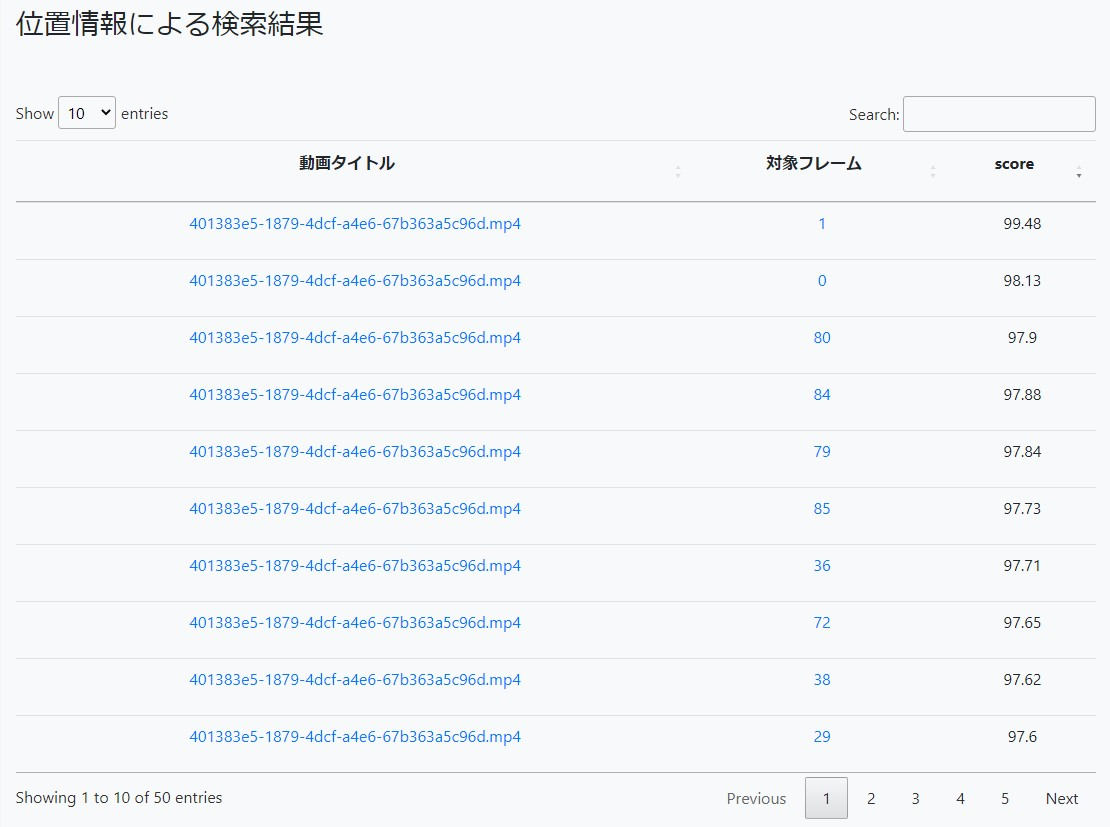
\includegraphics[width=13cm]{image/result_1_1_1.jpg}
  \caption{検証画像1-2}
  \label{fig:img_1-1-1}
\end{figure}
>>>>>>> parent of 36117c4 (考察増やした)

スコアが図\ref{fig:img_1-1-1}中にあるfps:80(スコア:97.9)のフレームの様子も図\ref{fig:img_1-1-2}に示す.
\begin{figure}[b]
  \centering
  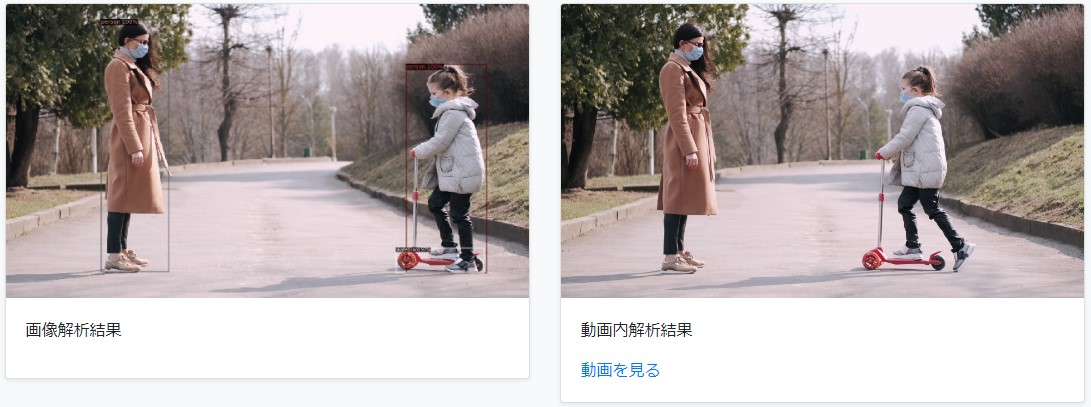
\includegraphics[width=13cm]{image/result_1_1_2.jpg}
  \caption{検証画像1-3}
  \label{fig:img_1-1-2}
\end{figure}

この80フレーム目でも検出しているオブジェクトが同じであり,そのオブジェクトの検出された座標が近いため,スコアが高く出力されていることがわかる.
このように,オブジェクトの位置が完全に一致していない場合でも,入力した画像と類似しているフレームがある場合は検索結果に表示される.
<<<<<<< HEAD
なお,出力されたフレーム数に出力すると,$0,1,13,15,..$とほぼフレーム順で類似シーンが出力されていることがわかる.
ちなみに,production ID\_4265040.mp4の動画データの詳細を見てみると表\ref{tab:tab_1_1_1}のようにおり,フレームレートが29.97であるため,
動画の秒数に換算しても,0秒〜1秒の間で類似シーンが存在していることがわかる.
\begin{table}[b]
  \centering
  \caption{production ID\_4265040.mp4の動画データの詳細}
  \label{tab:tab_1_1_1}
  \begin{tabular}{cc}
    \toprule
    \thead{項目} & \thead{数値} \\
    \midrule
    横の大きさ & 3840 \\
    縦の大きさ & 2160 \\
    フレームレート & 29.97 \\
    総フレーム数 & 510 \\
    長さ & 00:17 \\
    \bottomrule
  \end{tabular}
\end{table}

次に入力した画像と結果を図\ref{fig:img_1_2}に示す.
\begin{figure}[H]
=======

次に入力した画像と結果を図\ref{fig:img_1-2}に示す.
\begin{figure}[b]
>>>>>>> parent of 36117c4 (考察増やした)
  \centering
  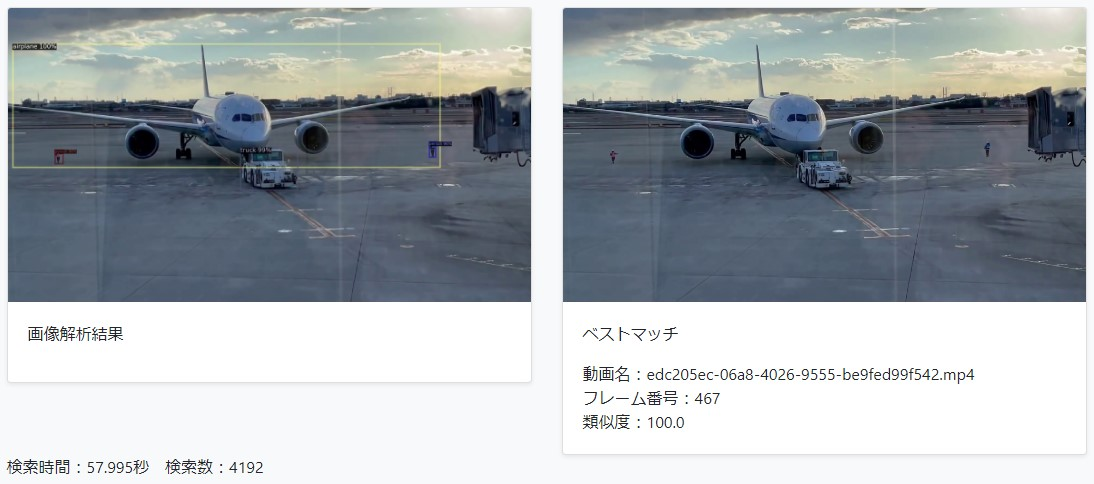
\includegraphics[width=13cm]{image/result_1_2.jpg}
  \caption{検証画像2}
  \label{fig:img_1-2}
\end{figure}

こちらの画像も検索したい動画のフレームを完全一致のフレームとして検索できていることがわかる.
オブジェクトは,airplaneとtruck,personが2つ検出されている.
画像とフレームのどちらも検出された座標が全く同じであるため,スコアが100として出力されている.

<<<<<<< HEAD
上位の検索結果を表\ref{tab:tab_1_2}に示す.
\begin{table}[b]
  \centering
  \caption{\ref{fig:img_1_2}の検出結果}
  \label{tab:tab_1_2}
  \begin{tabular}{ccc}
    \toprule
    \thead{動画タイトル} & \thead{対象フレーム} & \thead{score}  \\
    \midrule
    2022-12-31 & 467 & 100.0 \\
    2022-12-31 & 466 & 99.39 \\
    2022-12-31 & 465 & 98.97 \\
    2022-12-31 & 464 & 98.81 \\
    2022-12-31 & 468 & 98.52 \\
    2022-12-31 & 463 & 98.25 \\
    2022-12-31 & 469 & 97.83 \\
    2022-12-31 & 459 & 97.54 \\
    2022-12-31 & 470 & 97.31 \\
    2022-12-31 & 429 & 96.65 \\
    \bottomrule
  \end{tabular}
\end{table}

次に,3枚目の入力画像と結果を図\ref{fig:img_1_3}に示す.
\begin{figure}[H]
=======

次に,3枚目の入力画像と結果を図\ref{fig:img_1-3}に示す.
\begin{figure}[b]
>>>>>>> parent of 36117c4 (考察増やした)
  \centering
  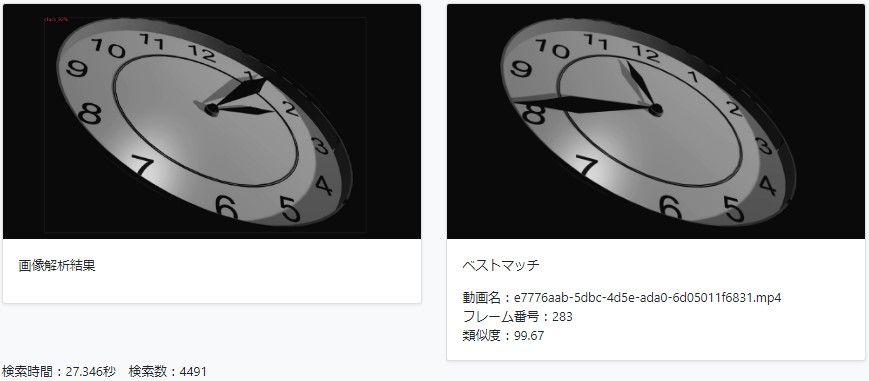
\includegraphics[width=13cm]{image/result_1_3.jpg}
  \caption{検証画像3}
  \label{fig:img_1-3}
\end{figure}

図\ref{fig:img_1-3}のでは,スコアが99.67とかなり高いスコアで検出されている.
しかし,2つの画像を比べてみると,検出しているフレームが異なっていることがわかる.

<<<<<<< HEAD
上位の検索結果を表\ref{tab:tab_1_3}に示す.
\begin{table}[b]
  \centering
  \caption{\ref{fig:img_1_3}の検出結果}
  \label{tab:tab_1_3}
  \begin{tabular}{ccc}
    \toprule
    \thead{動画タイトル} & \thead{対象フレーム} & \thead{score}  \\
    \midrule
    clock.mp4 & 283 & 99.67 \\
    clock.mp4 & 58 & 99.22 \\
    clock.mp4 & 8 & 99.21 \\
    clock.mp4 & 56 & 99.17 \\
    clock.mp4 & 187 & 99.16 \\
    clock.mp4 & 189 & 99.09 \\
    clock.mp4 & 52 & 99.04 \\
    clock.mp4 & 234 & 99.0 \\
    clock.mp4 & 2 & 98.98 \\
    clock.mp4 & 137 & 98.93 \\
    \bottomrule
  \end{tabular}
\end{table}

これまでの表\ref{tab:tab_1_1},表\ref{tab:tab_1_2}の出力では検出されたフレーム番号が近いものが多かったが,表\ref{tab:tab_1_3}の出力では検出されたフレーム番号が離れているものが見受けられた.

次に,4枚目の入力画像と結果を図\ref{fig:img_1_4}に示す.
\begin{figure}[H]
  \centering
  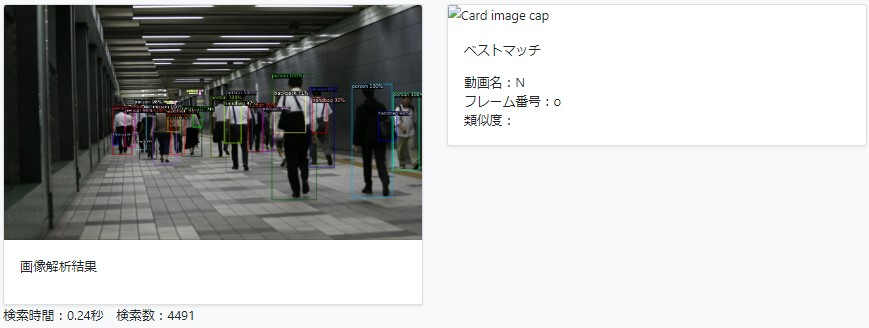
\includegraphics[width=13cm]{image/result_1_4.jpg}
  \caption{ディジタルヒューマンのイメージ画像}
  \label{fig:img_1_4}
\end{figure}

この画像は,図\ref{fig:movie4}の動画内で繰り返し出現するシーンの画像である.
図\ref{fig:img_1_4}の検出結果を表\ref{tab:tab_1_4}に示す.
\begin{table}[b]
  \centering
  \caption{\ref{fig:img_1_4}の検出結果}
  \label{tab:tab_1_4}
  \begin{tabular}{ccc}
    \toprule
    \thead{動画タイトル} & \thead{対象フレーム} & \thead{score}  \\
    \midrule
    ロボット-人間-オフィス-将来-88219.mp4 & 63 & 98.01 \\
    ロボット-人間-オフィス-将来-88219.mp4 & 149 & 97.51 \\
    ロボット-人間-オフィス-将来-88219.mp4 & 234 & 96.47 \\
    ロボット-人間-オフィス-将来-88219.mp4 & 62 & 96.31 \\
    ロボット-人間-オフィス-将来-88219.mp4 & 578 & 95.62 \\
    ロボット-人間-オフィス-将来-88219.mp4 & 496 & 88.17 \\
    \bottomrule
  \end{tabular}
\end{table}

表\ref{tab:tab_1_4}の出力では,検出されたフレーム番号が飛び飛びになっている.
これは,図\ref{fig:img_1_4}の画像が,図\ref{fig:movie4}の動画内で繰り返し出現するシーンの画像であるためである.
フレーム番号63と,フレーム番号149の結果を図\ref{fig:img_1_4_1},図\ref{fig:img_1_4_2}に示す.
\begin{figure}[H]
  \centering
  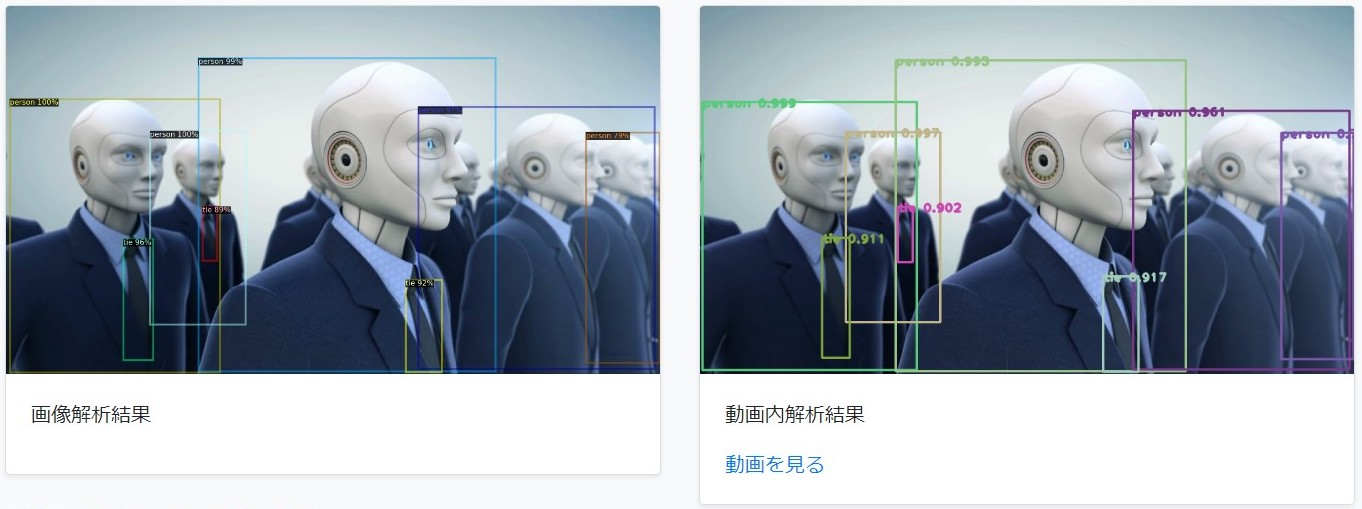
\includegraphics[width=13cm]{image/result_1_4_1.jpg}
  \caption{フレーム番号63の検出結果}
  \label{fig:img_1_4_1}
\end{figure}

\begin{figure}[H]
  \centering
  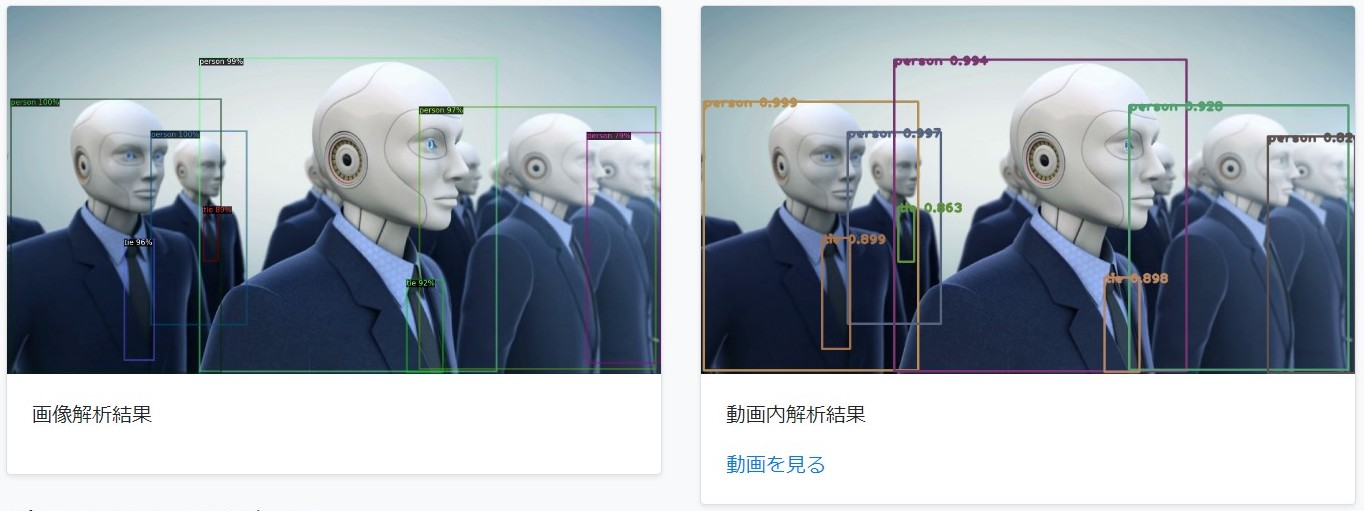
\includegraphics[width=13cm]{image/result_1_4_2.jpg}
  \caption{フレーム番号149の検出結果}
  \label{fig:img_1_4_2}
\end{figure}

どちらも同じようなシーンであるが,フレーム位置が異なっているためそれぞれのフレームの結果が表\ref{tab:tab_1_4}で出力されている.


最後に,オブジェクトが大量に映っている画像として5枚目の入力画像と結果を図\ref{fig:img_1_5}に示す.
\begin{figure}[H]
  \centering
  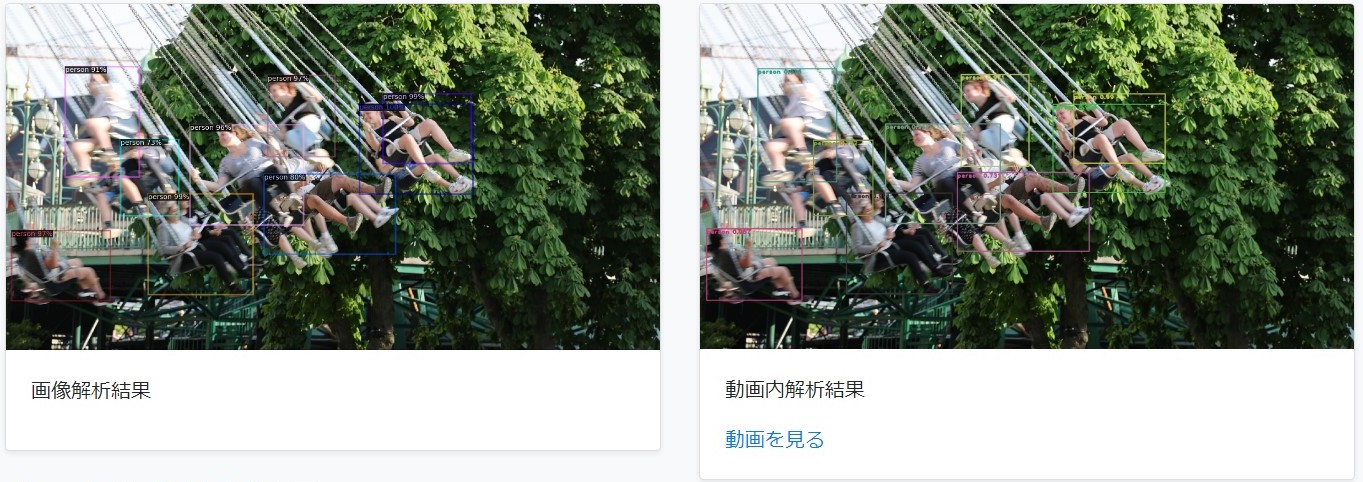
\includegraphics[width=13cm]{image/result_1_5.jpg}
  \caption{カルーセルの様子}
  \label{fig:img_1_5}
\end{figure}

図\ref{fig:img_1_5}では,スコアが98.54とほぼ一致したシーンの検出ができている.
これ以外に検出された類似シーンはなかった.
これまでと比べ,類似シーンの検索出力が少ないことがわかる.

他のシーンの画像でもシーン検索が行われるか確認したい.
その図を\ref{fig:img_1_5_1}に示す.
\begin{figure}[H]
  \centering
  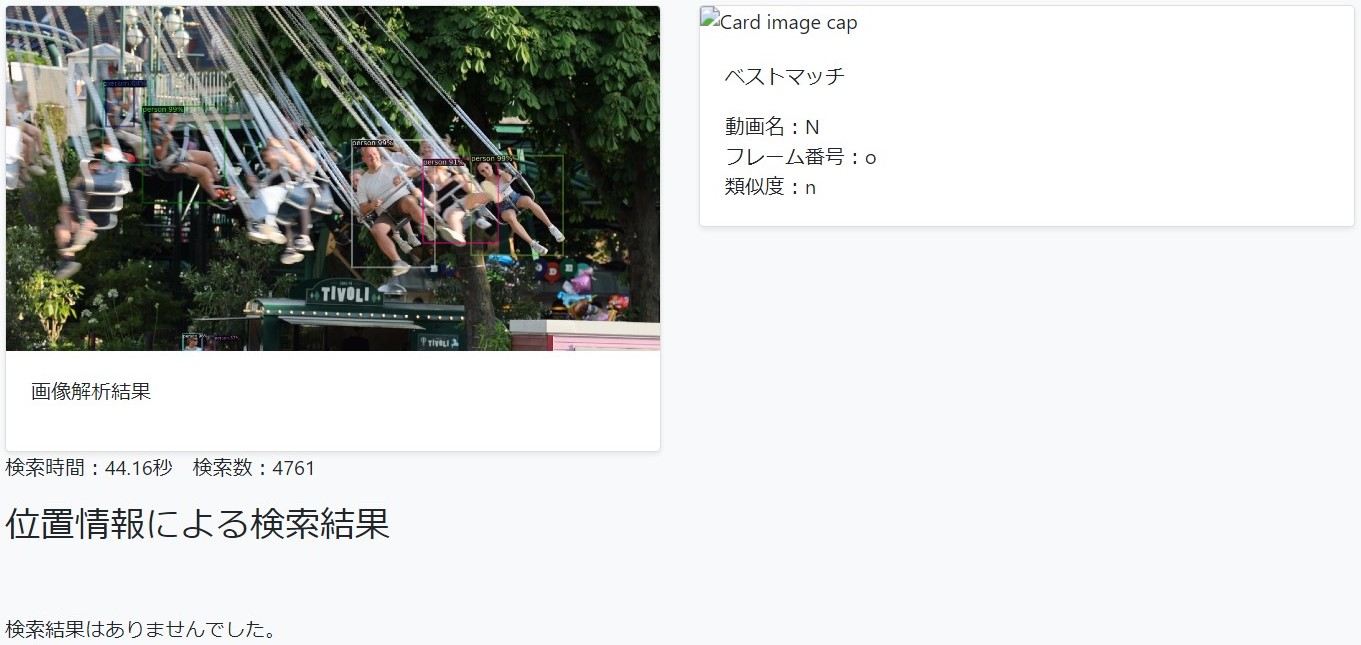
\includegraphics[width=13cm]{image/result_1_5_1.jpg}
  \caption{図\ref{fig:img_1_5}とは別のシーンのようす}
  \label{fig:img_1_5_1}
\end{figure}

図\ref{fig:img_1_5_1}のように,検索の結果の出力が得られなかった.

\subsection{考察}
入力した画像と近いシーンを検索することができた.
ほとんどの画像に対してスコアが95以上の高精度で出力されたことがわかる.

図\ref{fig:img_1_4}のような,同じシーンが繰り返し存在する動画に対しても,適切な検索がなされていることがわかった.

しかし,いくつか問題も見受けられた.
まず,図\ref{fig:img_1_3}の結果である.
検出精度がかなり高い割には,検出されたシーン(フレーム)にばらつきが見られる.
入力された画像と針の位置が類似していないように見える.

これは,この検索対象となった図\ref{fig:movie3}は,時計自体の位置は固定されており,針の位置だけが変化している動画だからこそ起こる現象であると考えられる.
本システムの検索システムの特徴として,オブジェクトとして認識されるのは,事前に学習させたクラスのみとなっている.
今回使用している学習済みモデルは,COCOデータセットで学習させたモデルであるため,時計の針に関するクラスは存在せず,時計自体のクラスのみが検出された.
そのため,全てのフレームがほぼ一致しているシーンとみなされてしまっている.
=======
この検索対象となった図\ref{fig:movie3}は,時計自体の位置は固定されており,針の位置だけが変化しているため,全てのフレームがほぼ一致しているシーンとみなされてしまうためである.
>>>>>>> parent of 36117c4 (考察増やした)

本システムでは,検索対象がオブジェクト名と検出された座標であるため,その2つを満たしているフレームであれば,一致シーンとして出力される.
オブジェクトの色が異なったり,オブジェクトの向きが異なったりしても,検出された座標が同じであれば,一致シーンとして出力されてしまうことがわかった.

最後に,4枚目の入力画像と結果を図\ref{fig:img_1-4}に示す.
\begin{figure}[b]
  \centering
  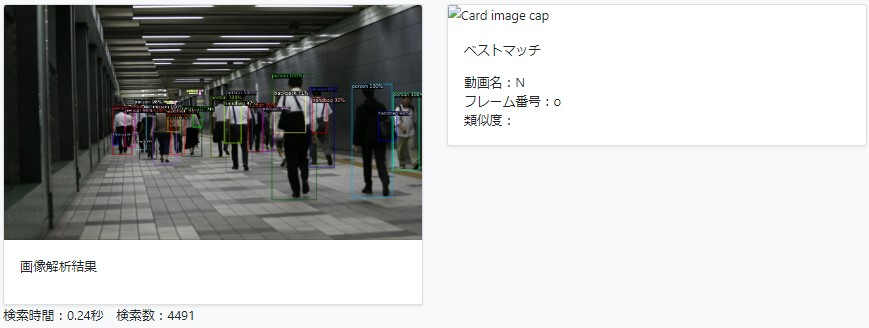
\includegraphics[width=13cm]{image/result_1_4.jpg}
  \caption{検証画像4}
  \label{fig:img_1-4}
\end{figure}

図\ref{fig:img_1-4}のように,検出数がとても多い場合は,動画から検出されにくいことがわかった.
検索の条件として,検出したオブジェクト数および名称が一致していること,そしてその検出座標が近いことを満たしている場合のみ,一致シーンとして出力するようにしている.
本来,検索対象となるべき動画(図\ref{fig:movie4})は,大量のオブジェクトが検出されており,オブジェクトが少しでも重なると検出数が異なってしまうため,検索対象となりずらいことがわかった.
今回入力した画像はオブジェクトの検出数が表\ref{tab:tab_1_4}のように22個のオブジェクト認識となっているが,これらのデータと一致するシーンは見つからなかったことになる.

\begin{table}[b]
  \centering
  \caption{\ref{fig:img_1-4}の検出結果}
  \label{tab:tab_1_4}
  \begin{tabular}{ccccccc}
    \toprule
    \thead{オブジェクト名} & \thead{検出率} & \thead{x-min} & \thead{y-min} & \thead{x-max} & \thead{y-max}  \\
    \midrule
    backpack & 0.7102 & 0.6465 & 0.3665 & 0.7211 & 0.5418 \\
    handbag & 0.9729 & 0.5266 & 0.4105 & 0.5668 & 0.5869 \\
    handbag & 0.9437 & 0.8950 & 0.4529 & 0.9384 & 0.5766 \\
    handbag & 0.9235 & 0.7372 & 0.3970 & 0.7705 & 0.5439 \\
    handbag & 0.9130 & 0.2605 & 0.5448 & 0.2715 & 0.5970 \\
    handbag & 0.9097 & 0.3876 & 0.4609 & 0.4124 & 0.5314 \\
    handbag & 0.8335 & 0.3085 & 0.5411 & 0.3184 & 0.5770 \\
    handbag & 0.7201 & 0.3918 & 0.4709 & 0.4213 & 0.5391 \\
    person & 0.9992 & 0.6407 & 0.2928 & 0.7475 & 0.8278 \\
    person & 0.9990 & 0.8322 & 0.3371 & 0.9275 & 0.8164 \\
    person & 0.9986 & 0.5305 & 0.3647 & 0.5934 & 0.7102 \\
    person & 0.9986 & 0.2606 & 0.4307 & 0.3058 & 0.6362 \\
    person & 0.9966 & 0.4250 & 0.4311 & 0.4727 & 0.6436 \\
    person & 0.9964 & 0.4950 & 0.3856 & 0.5390 & 0.6470 \\
    person & 0.9964 & 0.9306 & 0.3731 & 0.9923 & 0.7026 \\
    person & 0.9959 & 0.3559 & 0.4252 & 0.4119 & 0.6760 \\
    person & 0.9941 & 0.7314 & 0.3502 & 0.7897 & 0.6901 \\
    person & 0.9920 & 0.5839 & 0.4181 & 0.6187 & 0.6231 \\
    person & 0.9816 & 0.3238 & 0.4390 & 0.3640 & 0.6546 \\
    person & 0.9769 & 0.3989 & 0.4415 & 0.4311 & 0.6369 \\
    person & 0.9645 & 0.2892 & 0.4402 & 0.3128 & 0.6037 \\
    person & 0.9623 & 0.3116 & 0.4041 & 0.3404 & 0.6154 \\
    \bottomrule
  \end{tabular}
\end{table}

このように,オブジェクトの数があまりにも多い場合や,オブジェクトの移動がない動画を除いて,基本的な検索機能を実装することができた.

\section{位置関係を用いた検索システムについて}
位置情報を用いた検索システムの精度についても考える.

<<<<<<< HEAD
前のセクションで用いた4つの動画に加え,図\ref{fig:movie6}も検索対象として用いる.
図\ref{fig:movie6}は,新しい解析対象の動画として加えた,少年がスポーツカーに手を振っている様子を撮影した動画である.
\begin{figure}[H]
  \centering
  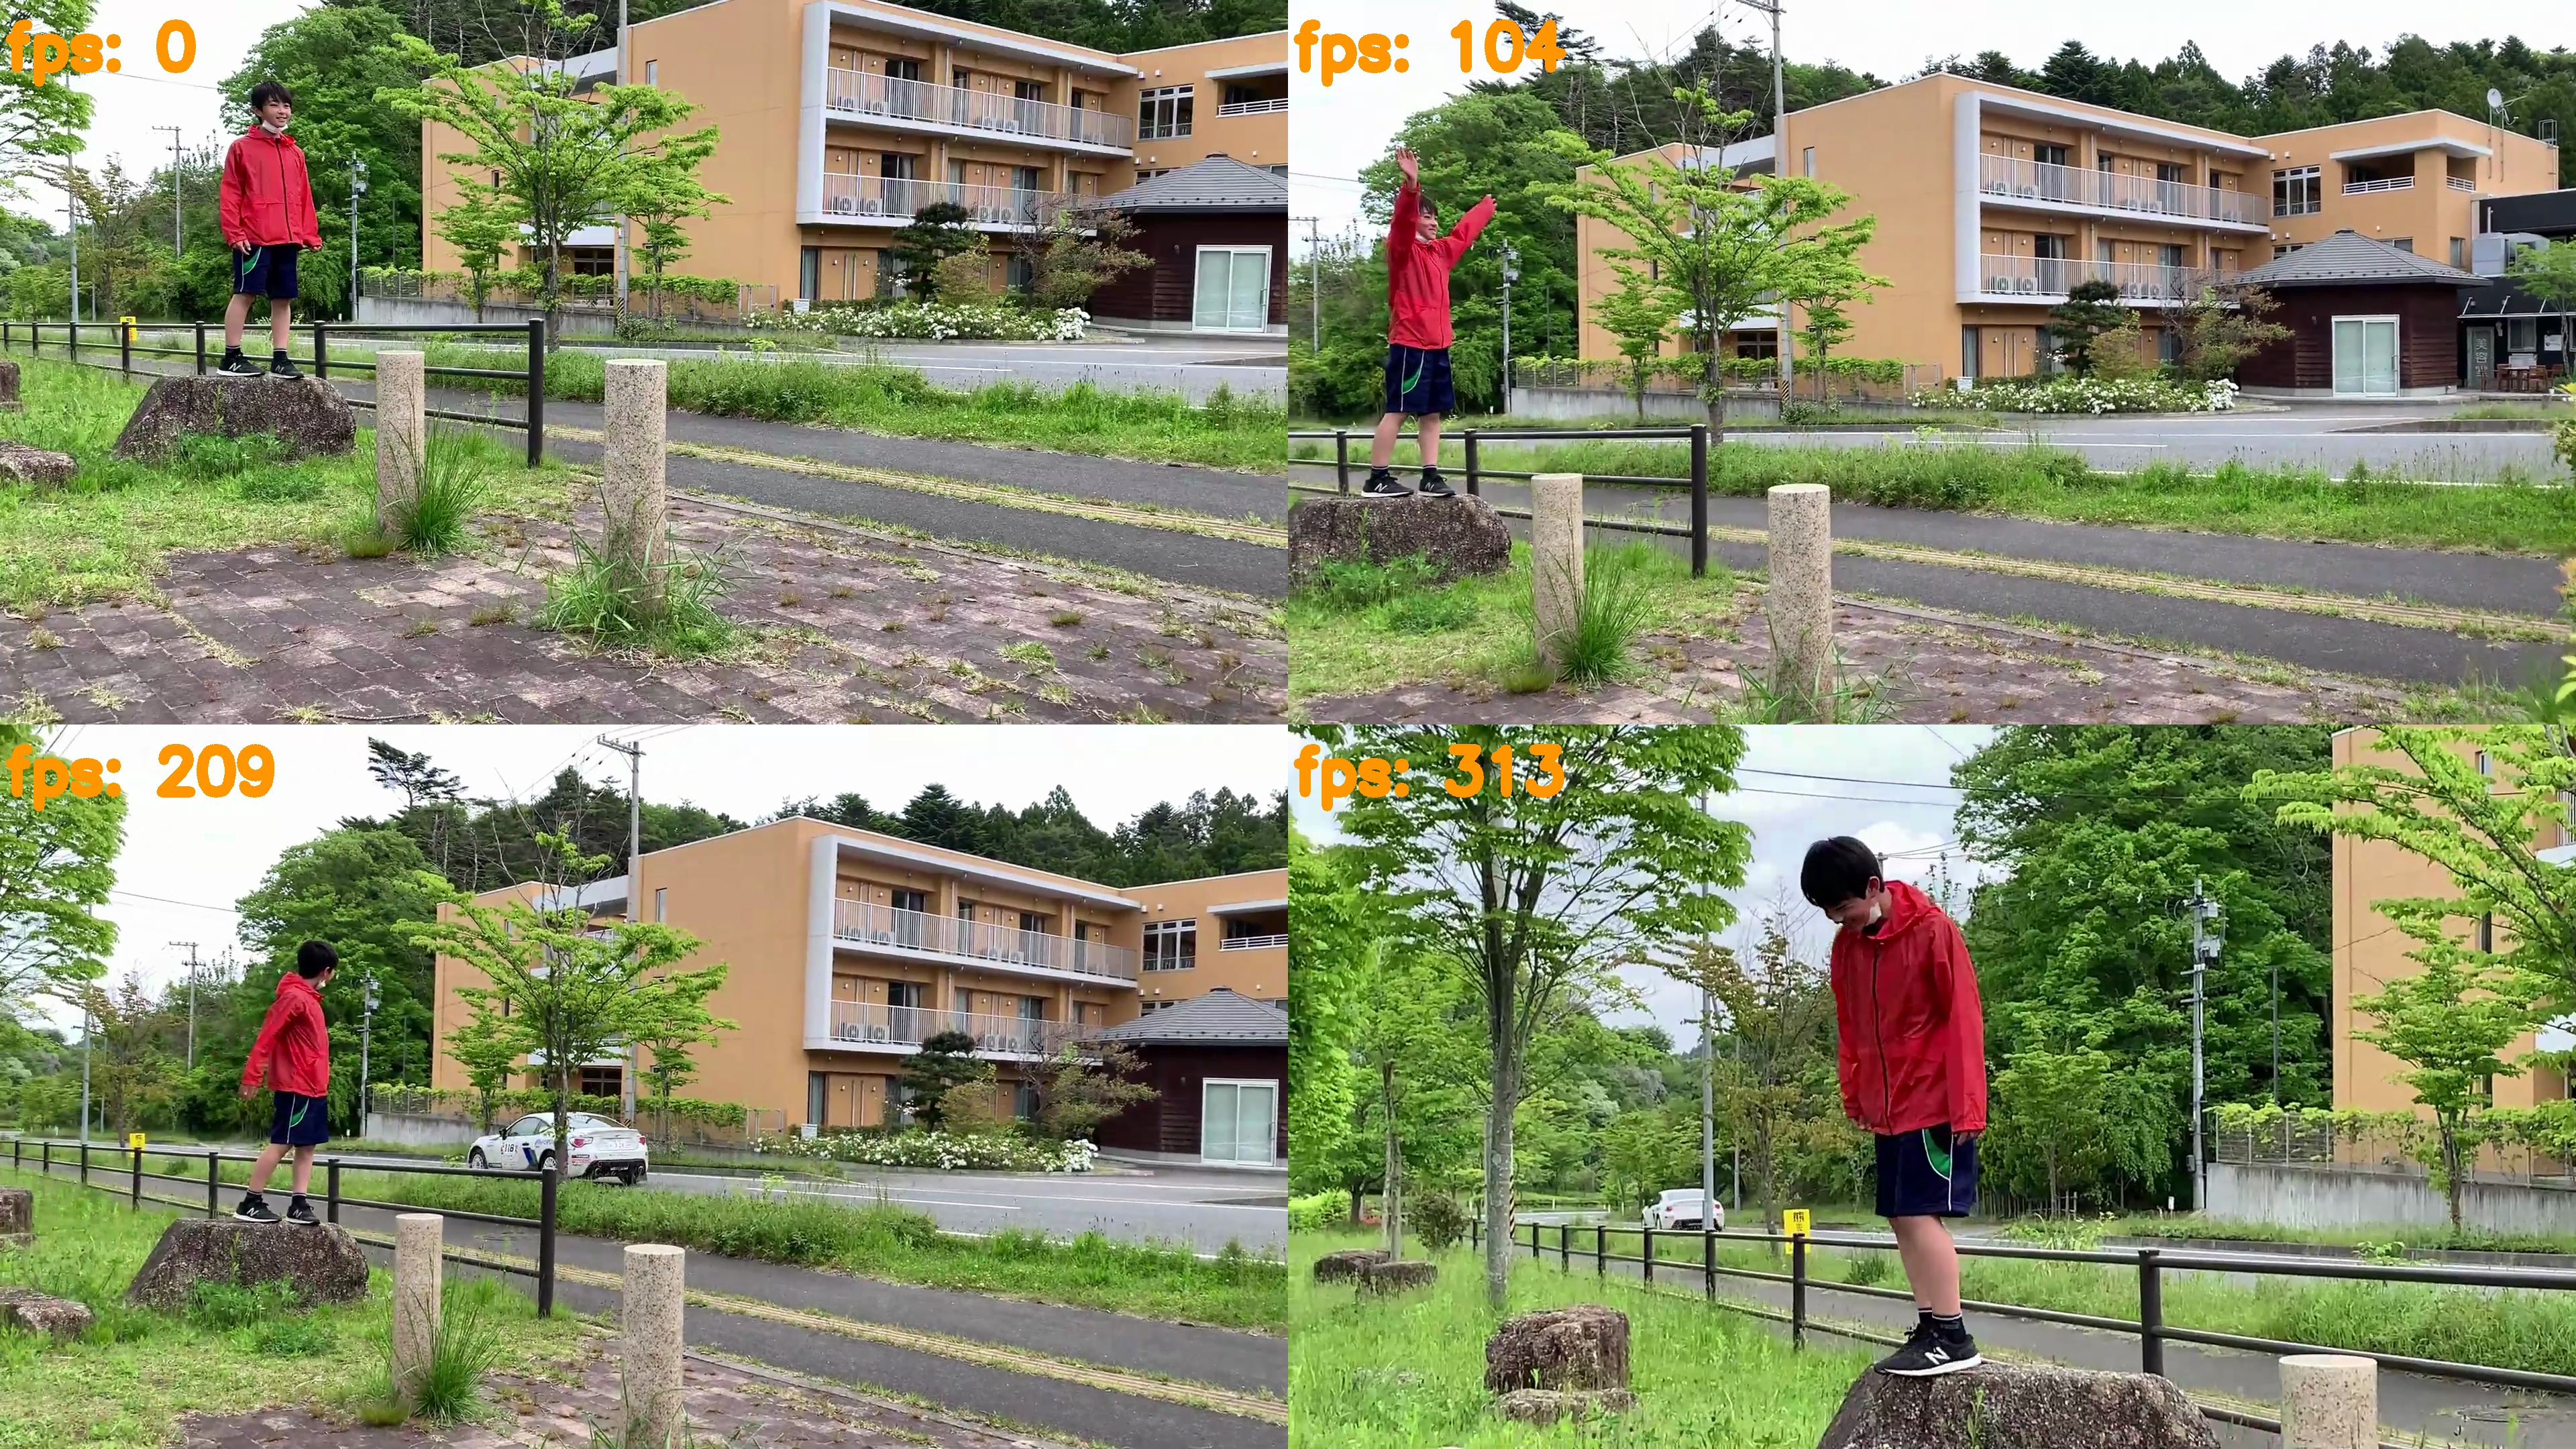
\includegraphics[width=13cm]{image/6_result.jpg}
  \caption{少年がスポーツカーに手を振っている動画}
  \label{fig:movie6}
\end{figure}

また,類似するシーンが存在している動画2つも検索対象として用いる(図\ref{fig:movie7}と図\ref{fig:movie8}).
\begin{figure}[H]
  \centering
  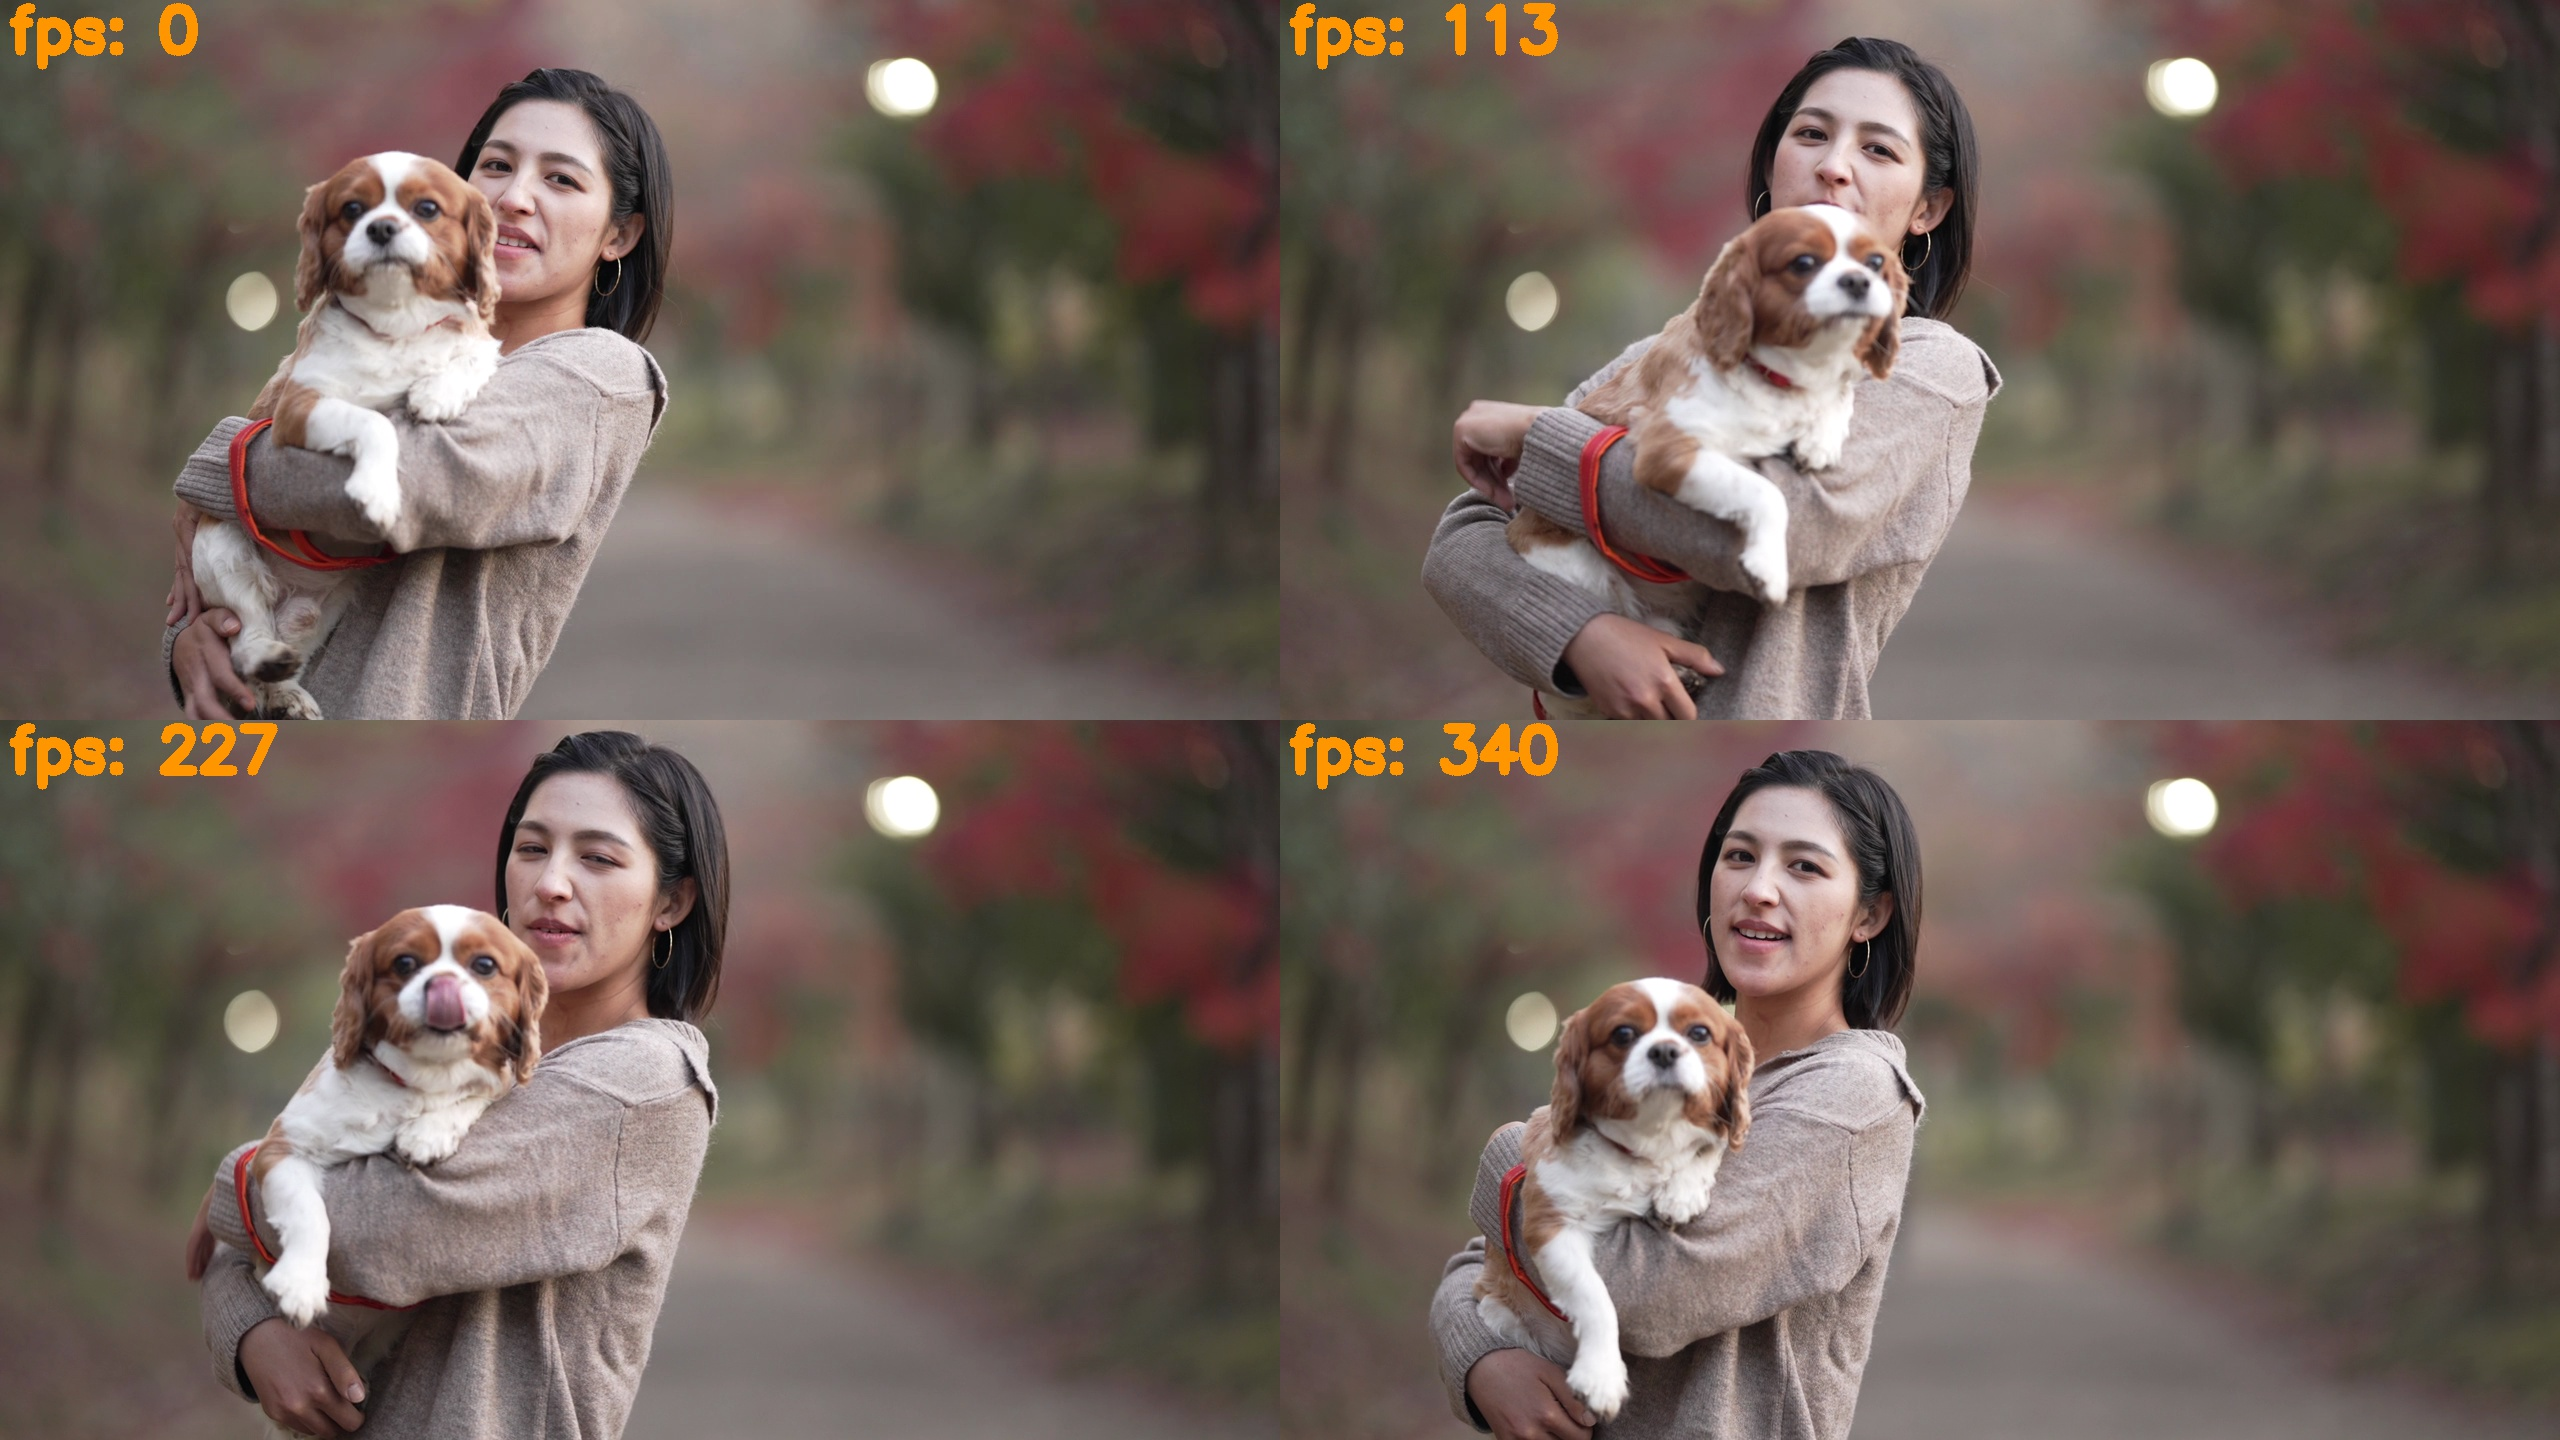
\includegraphics[width=13cm]{image/7_result.jpg}
  \caption{人と犬が映っている動画 その1}
  \label{fig:movie7}
\end{figure}

\begin{figure}[H]
  \centering
  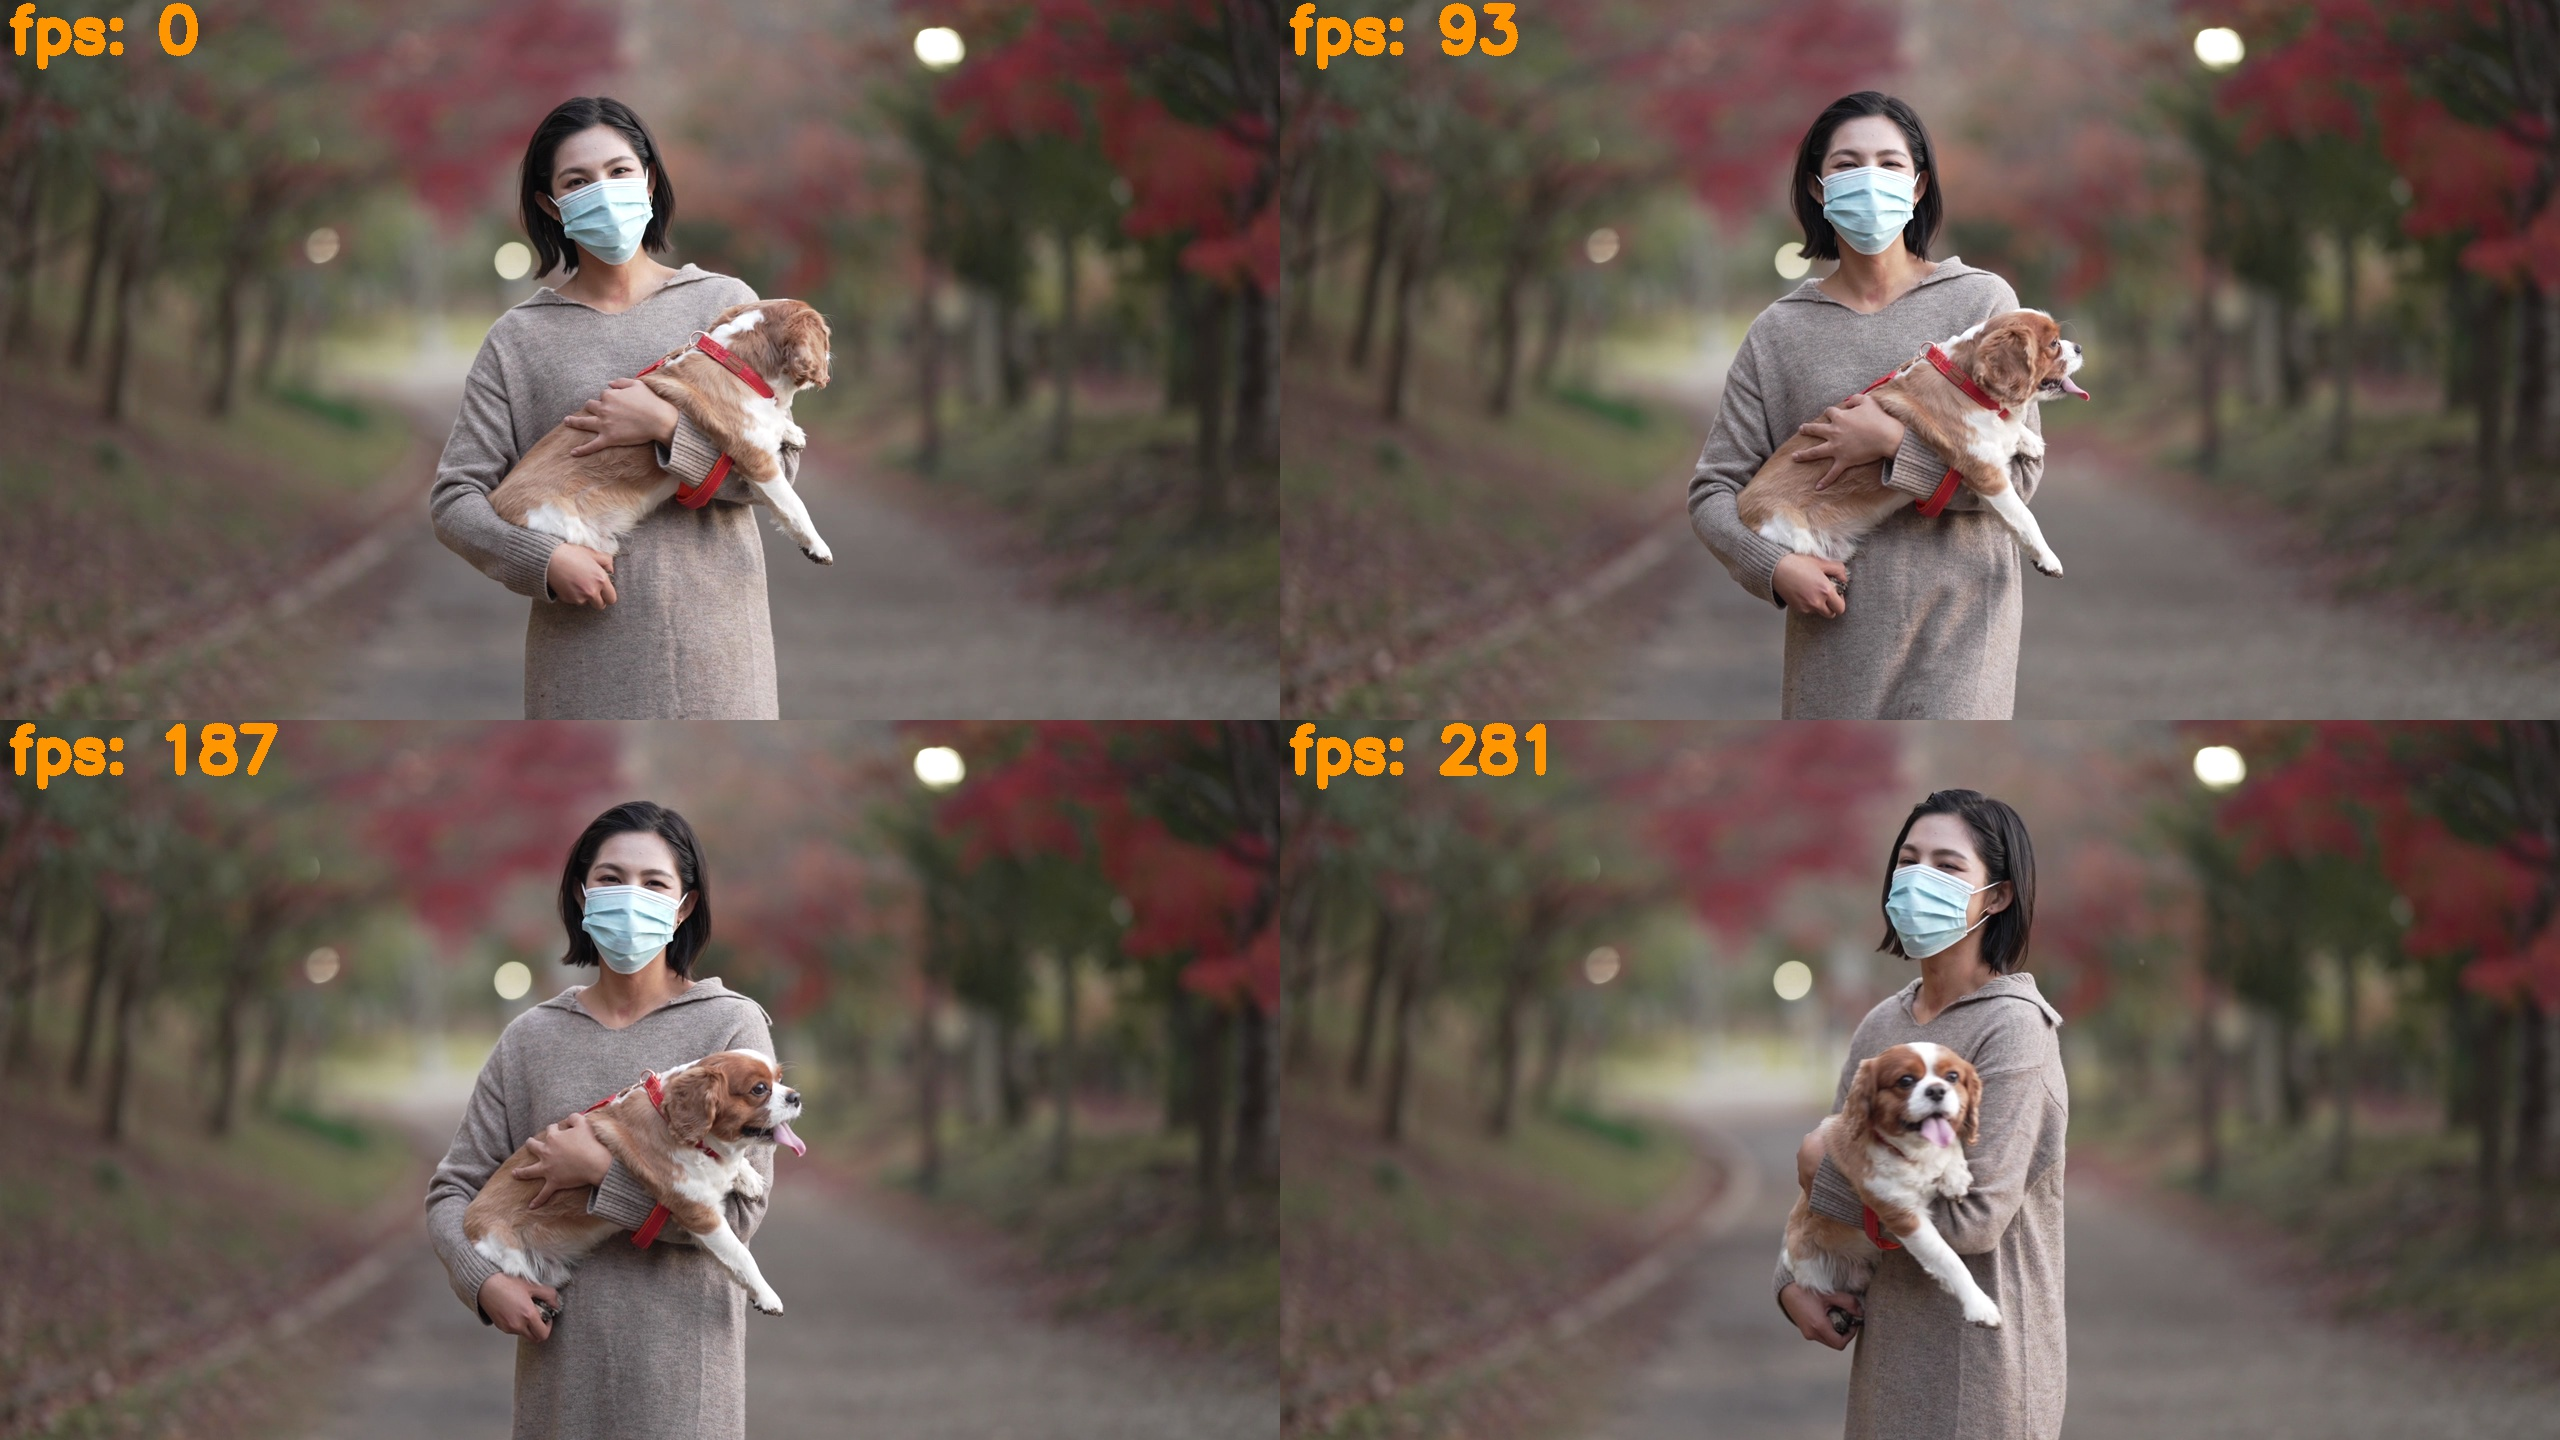
\includegraphics[width=13cm]{image/8_result.jpg}
  \caption{人と犬が映っている動画 その2}
  \label{fig:movie8}
=======
前のセクションで用いた4つの動画に加え,図\ref{fig:movie5}も検索対象として用いる.
図\ref{fig:movie5}は,新しい解析対象の動画として加えた,少年がスポーツカーに手を振っている様子を撮影した動画である.
\begin{figure}[b]
  \centering
  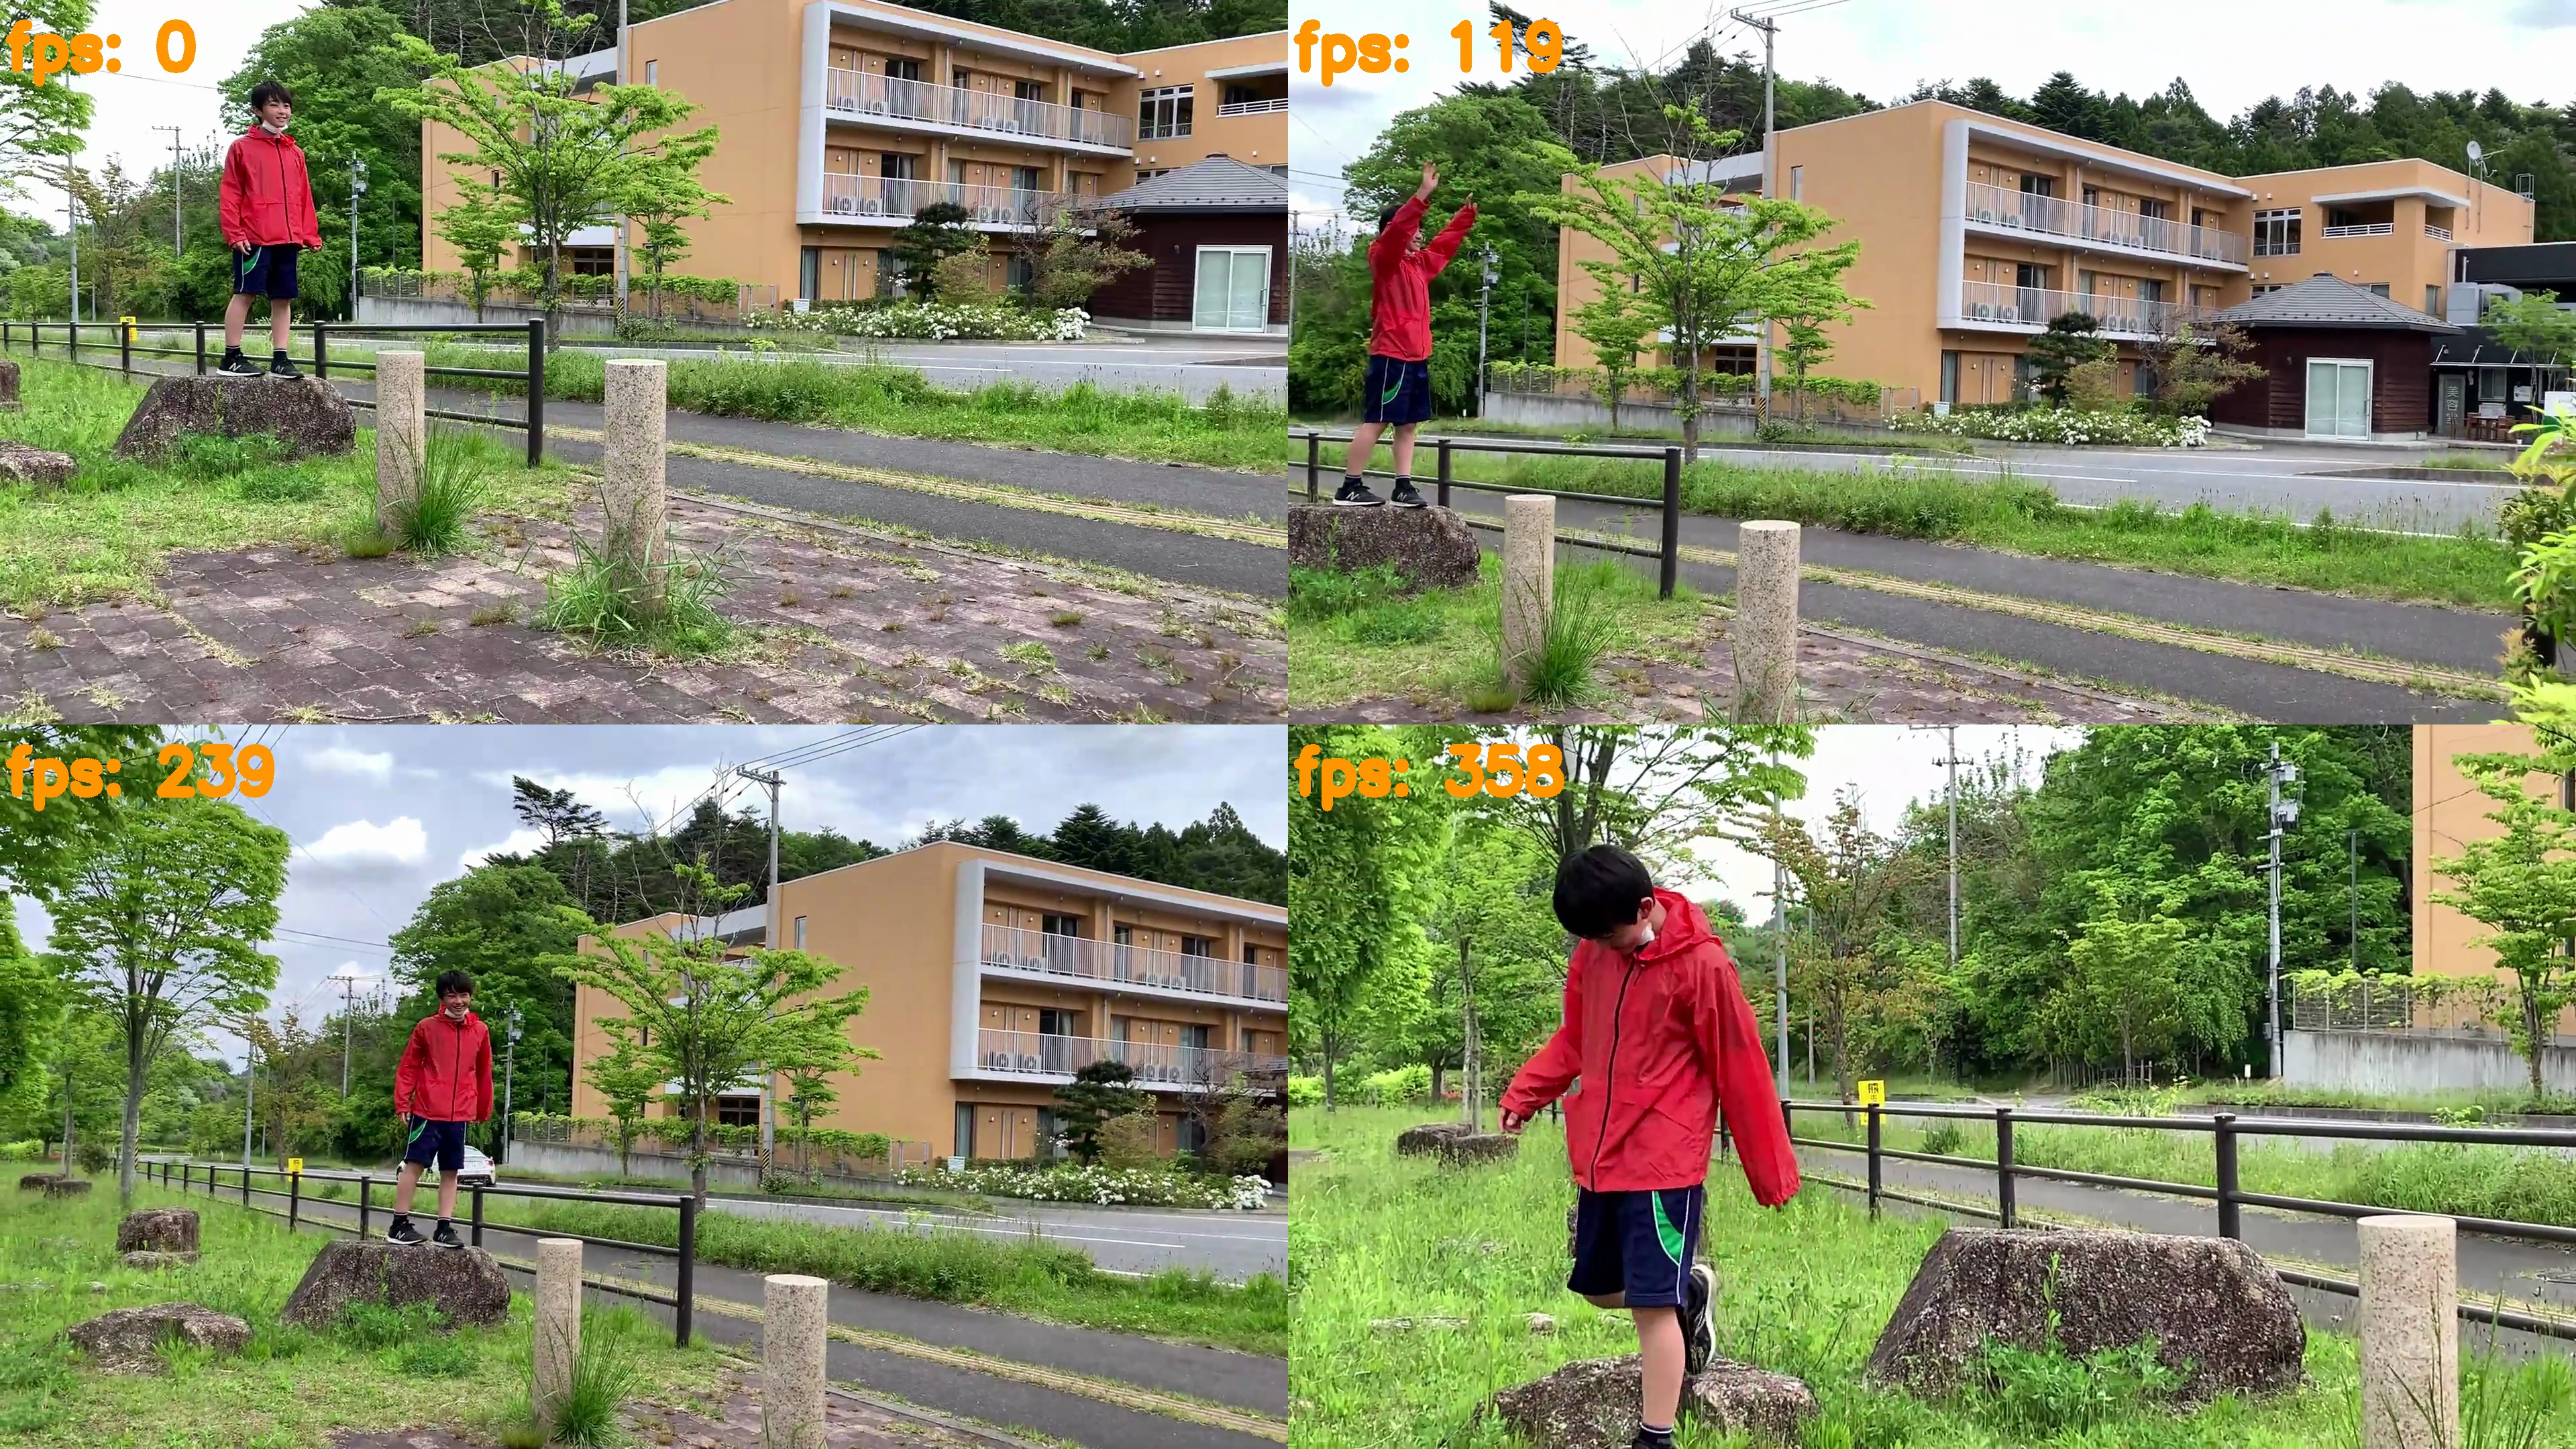
\includegraphics[width=13cm]{image/5_result.jpg}
  \caption{動画5つ目}
  \label{fig:movie5}
>>>>>>> parent of 36117c4 (考察増やした)
\end{figure}

次に入力した画像と結果を示す.

まず,図\ref{fig:img_1-2}の時の,類似シーンの検索結果を図\ref{fig:img_2-1}に示す.
\begin{figure}[b]
  \centering
<<<<<<< HEAD
  \caption{図\ref{fig:img_1_2}の検出結果(【角度の分散】で昇順ソート)}
  \label{tab:tab_2_1}
  \begin{tabular}{cccccc}
    \toprule
    \thead{動画タイトル} & \thead{対象フレーム} & \thead{図形の傾き} & \thead{長さの平均} & \thead{長さの分散} & \thead{角度の分散} \\
    \midrule
    2022-12-31.mp4 & 467 & 0.0 & 1.0 & 0.0 & 0.0 \\
    2022-12-31.mp4 & 459 & 0.13 & 0.9953 & 0.0 & 0.0069 \\
    2022-12-31.mp4 & 464 & 0.09 & 0.9986 & 0.0 & 0.034 \\
    2022-12-31.mp4 & 463 & 0.22 & 0.9963 & 0.0002 & 0.0493 \\
    2022-12-31.mp4 & 453 & 0.06 & 1.2929 & 0.0002 & 0.0497 \\
    2022-12-31.mp4 & 466 & 0.1567 & 0.9997 & 0.0001 & 0.0557 \\
    2022-12-31.mp4 & 465 & 0.19 & 0.9995 & 0.0001 & 0.0718 \\
    2022-12-31.mp4 & 429 & 0.7167 & 0.9858 & 0.0001 & 0.0728 \\
    2022-12-31.mp4 & 257 & 0.2933 & 1.3556 & 0.0096 & 0.1384 \\
    2022-12-31.mp4 & 468 & 0.3267 & 1.0025 & 0.0005 & 0.1405 \\
    \bottomrule
  \end{tabular}
\end{table}

=======
  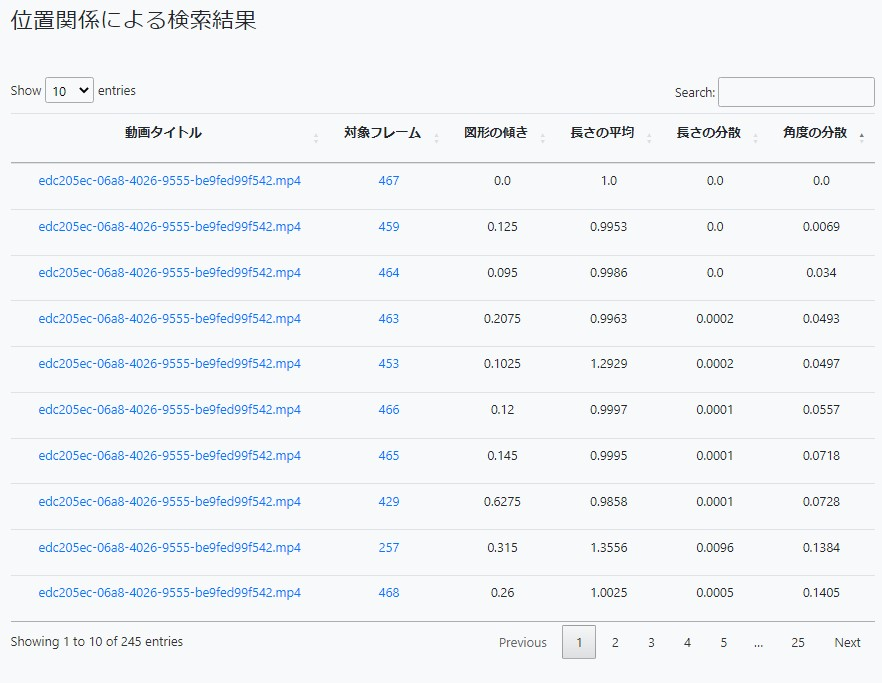
\includegraphics[width=13cm]{image/result_2_1.jpg}
  \caption{検証結果}
  \label{fig:img_2-1}
\end{figure}
>>>>>>> parent of 36117c4 (考察増やした)

一番上に表示されている467フレームは,前のセクションの検証画像2と同じシーンで,検出されたオブジェクトの位置関係にズレがないことがわかる.
フレーム番号459のシーンを図\ref{fig:img_2-1-2}に示す.

\begin{figure}[H]
  \centering
  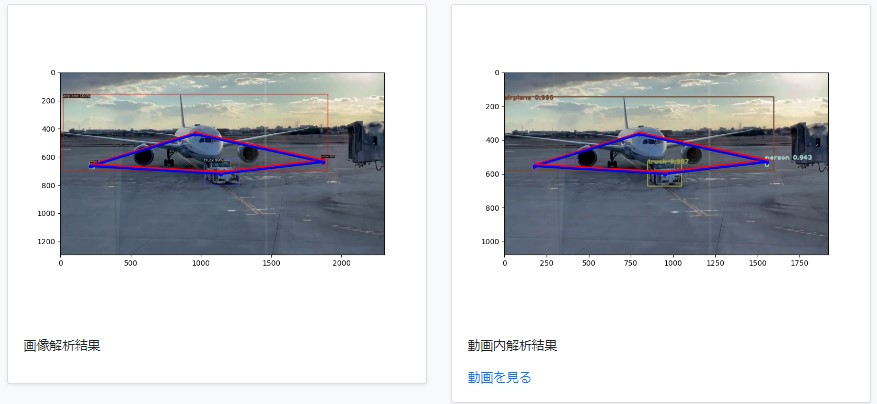
\includegraphics[width=13cm]{image/result_2_1_2.jpg}
<<<<<<< HEAD
  \caption{図\ref{fig:img_1_2}の459フレームでの検出結果}
  \label{fig:img_2_1_2}
=======
  \caption{検証結果}
  \label{fig:img_2-1-2}
>>>>>>> parent of 36117c4 (考察増やした)
\end{figure}

図\ref{fig:img_2-1-2}の左側は入力した画像で,右側は検索結果のフレームである.
なお,それぞれのオブジェクトの中心座標を線で結んで,オブジェクトの位置関係を示しており,赤色は画像の位置関係,青色は検索結果の位置関係を示している.
この2つの図形はほぼ一致しており,位置関係が類似していることがわかる.
<<<<<<< HEAD
表\ref{tab:tab_2_1}のデータより,角度の分散が$0.0069$,長さの平均が$0.9953$,傾きも$0.13$と,入力画像の位置関係とほぼ一致していることがわかる.
=======
図\ref{fig:img_2-1}のデータでは,角度の分散が0.0069,長さの平均が0.9953,傾きも0.125と,入力画像の位置関係とほぼ一致していることがわかる.
>>>>>>> parent of 36117c4 (考察増やした)

また,フレーム番号453のシーンを図\ref{fig:img_2-1-3}に示す.

\begin{figure}[H]
  \centering
  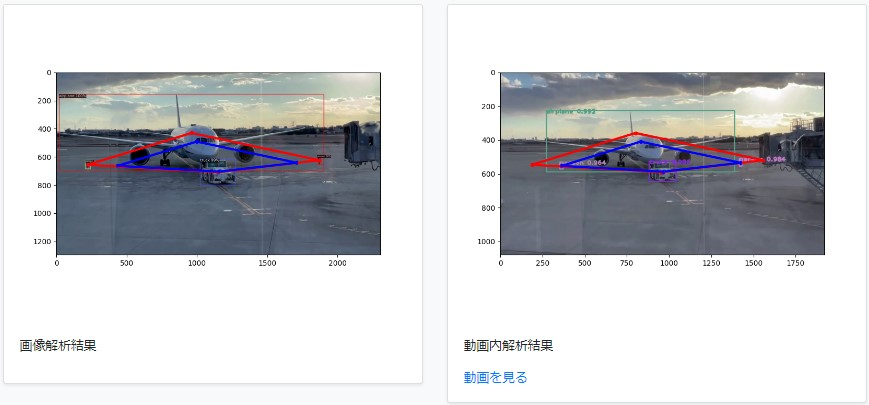
\includegraphics[width=13cm]{image/result_2_1_3.jpg}
<<<<<<< HEAD
  \caption{図\ref{fig:img_1_2}の453フレームでの検出結果}
  \label{fig:img_2_1_3}
\end{figure}

この図\ref{fig:img_2_1_3}の赤い線と青い線の関係が,相似であるかのように見える.
表\ref{tab:tab_2_1}のデータ中で,角度の分散が$0.0497$,図形の傾きが$0.06$と小さい値の中,長さの平均が$1.2929$となっている.
これより,図形の角度がほぼ一致しているが,図形自体の大きさが異なっていることがわかる.
実際,図\ref{fig:img_2_1_3}では,画像よりも少し画角の引かれたシーンが類似シーンとして出力されている.

また,参考として,傾きが一番大きいフレーム番号68のシーンを図\ref{fig:img_2_1_4}に示す.
\begin{figure}[H]
  \centering
  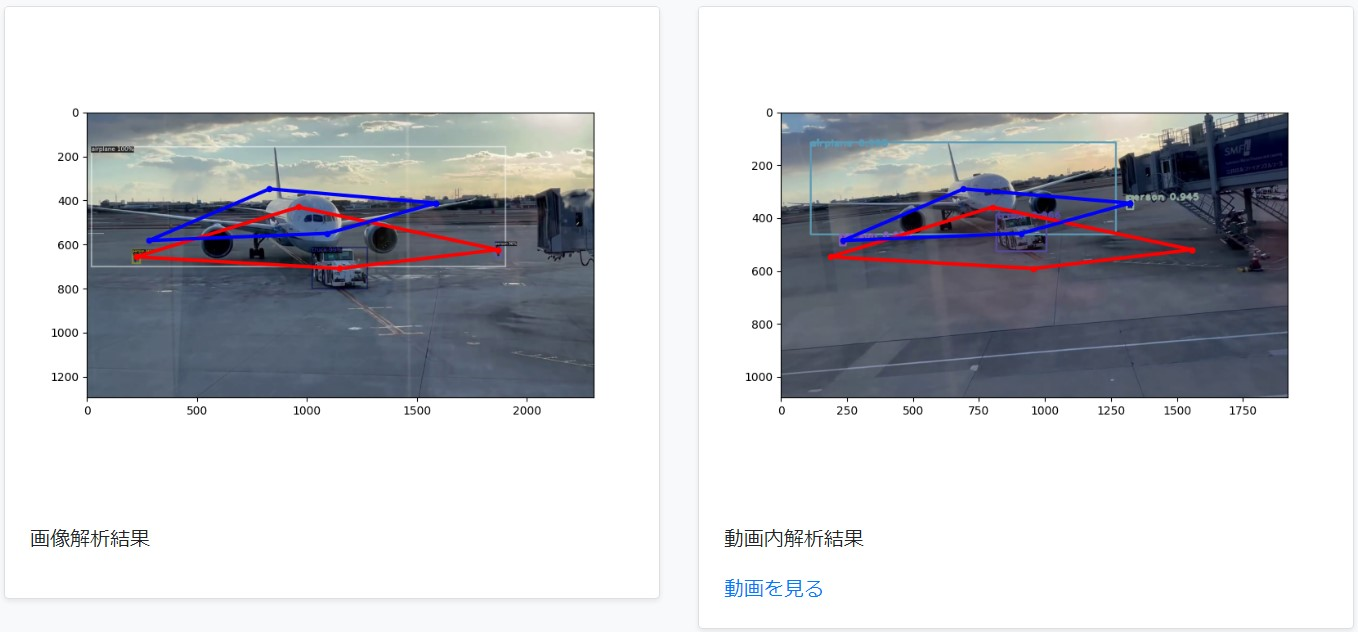
\includegraphics[width=13cm]{image/result_2_1_4.jpg}
  \caption{図\ref{fig:img_1_2}の68フレームでの検出結果}
  \label{fig:img_2_1_4}
\end{figure}

図\ref{fig:img_2_1_4}の赤い線と青い線の関係は,傾きが$6.28$と検索結果の中で最大である.
長さの平均は$1.2675$,長さの分散は$0.0102$,角度の分散は$3.6179$となっている.
こういった動画の中で,図形の位置関係が類似している場合は,動画内で傾いたシーンであっても検索結果として出力できることがわかった.

このように,先ほどのセクションの検索では検索対象として表示されなかったシーンまで,より幅広い検索が可能となった.

他の画像についても同様に検索を行った.

入力した画像を図\ref{fig:img_2_2_1}に示し,検索結果上位項目を表\ref{tab:tab_2_2}に示す.

\begin{figure}[H]
=======
  \caption{検証結果}
  \label{fig:img_2-1-3}
\end{figure}

この図\ref{fig:img_2-1-3}の赤い線と青い線の関係が,相似であるかのように見える.
図\ref{fig:img_2-1}のデータ中で,角度の分散が0.0497,図形の傾きが0.1025と小さい値の中,長さの平均が1.2929となっている.
これより,図形の角度がほぼ一致しているが,図形自体の大きさが異なっていることがわかる.
実際,図\ref{fig:img_2-1-3}では,画像よりも少し画角の引かれたシーンが類似シーンとして出力されている.
このように,先ほどのセクションの検索では検索対象として表示されなかったシーンまで,より幅広い検索が可能となった.

次に,この位置関係を用いた検索でしか出来ない検索を行う.
図\ref{fig:img_2-2}に示すように,動画中から欲しいシーンを他のアプリケーションで作り,検索を行ってみる.
なお,図\ref{fig:img_2-2}では,少年が手を振っている前を車が通過するシーンを動画中から検索するために作成した画像である.
\begin{figure}[b]
>>>>>>> parent of 36117c4 (考察増やした)
  \centering
  \fbox{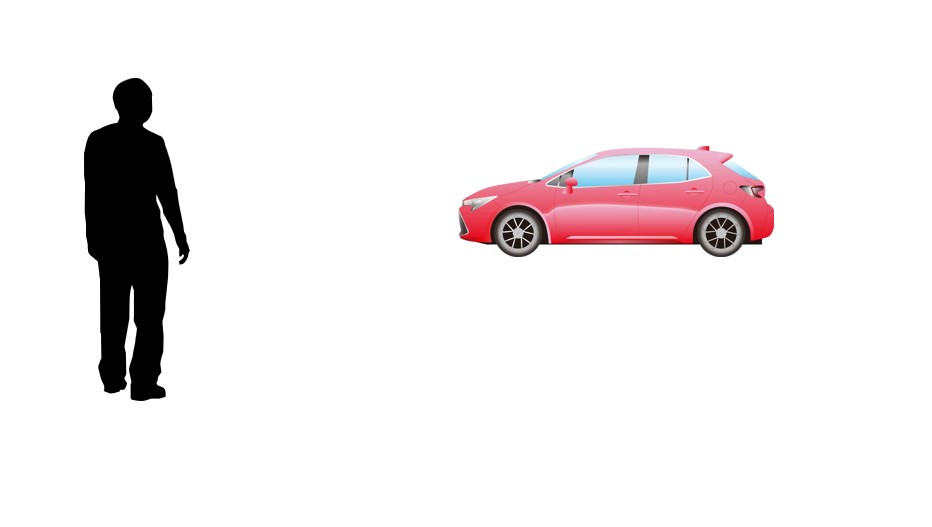
\includegraphics[width=13cm]{image/result_2_2.jpg}}
  \caption{入力画像}
  \label{fig:img_2-2}
\end{figure}

<<<<<<< HEAD
\begin{table}[t]
  \centering
  \caption{図\ref{fig:img_2_2_1}の検出結果(【図形の傾き】で昇順ソート)}
  \label{tab:tab_2_2}
  \begin{tabular}{cccccc}
    \toprule
    \thead{動画タイトル} & \thead{対象フレーム} & \thead{図形の傾き} & \thead{長さの平均} & \thead{長さの分散} & \thead{角度の分散} \\
    \midrule
    犬をカメラ目線にして記念撮影する女性.mp4 & 162 & 0.01 & 1.0059 & 0.0 & 0.0 \\
    犬をカメラ目線にして記念撮影する女性.mp4 & 197 & 0.04 & 0.9053 & 0.0 & 0.0 \\
    犬をカメラ目線にして記念撮影する女性.mp4 & 348 & 0.04 & 0.7887 & 0.0 & 0.0 \\
    犬をカメラ目線にして記念撮影する女性.mp4 & 349 & 0.04 & 0.7825 & 0.0 & 0.0 \\
    犬をカメラ目線にして記念撮影する女性.mp4 & 169 & 0.1 & 0.8994 & 0.0 & 0.0 \\
    犬をカメラ目線にして記念撮影する女性.mp4 & 181 & 0.1 & 0.8625 & 0.0 & 0.0 \\
    犬をカメラ目線にして記念撮影する女性.mp4 & 390 & 0.18 & 0.7998 & 0.0 & 0.0 \\
    犬を抱いてその場で回るマスクの女性.mp4 & 292 & 0.18 & 0.9966 & 0.0 & 0.0 \\
    犬をカメラ目線にして記念撮影する女性.mp4 & 129 & 0.22 & 1.6378 & 0.0 & 0.0 \\
    犬をカメラ目線にして記念撮影する女性.mp4 & 203 & 0.23 & 0.9194 & 0.0 & 0.0 \\
    \bottomrule
  \end{tabular}
\end{table}

表\ref{tab:tab_2_2}中の動画タイトルに注目すると,複数の動画から類似シーンを検出していることがわかる.
また,長さの分散と角度の分散がすべて0.0という出力になっていることもわかる.
検出されたオブジェクトが2つのため,角度が存在しない.そのため,図形の傾きと長さの平均のみの出力となっている.

図形の傾きの値が番小さい小さいフレーム番号355と,動画タイトルが他の結果と異なっているフレーム番号292の結果を図\ref{fig:img_2_2_3},図\ref{fig:img_2_2_4}に示す.
\begin{figure}[H]
=======
検索結果を図\ref{fig:img_2-2-1}に示す.
\begin{figure}[b]
>>>>>>> parent of 36117c4 (考察増やした)
  \centering
  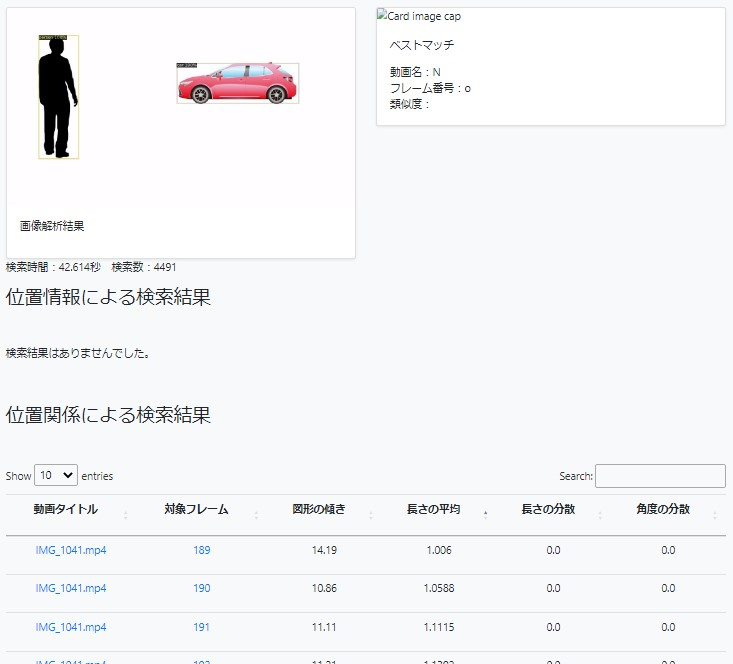
\includegraphics[width=13cm]{image/result_2_2_1.jpg}
  \caption{検索結果}
  \label{fig:img_2-2-1}
\end{figure}

図\ref{fig:img_2-2-1}のように,位置情報を用いた検索では検索結果が無いが,位置関係を用いた検索では,検索結果が出力された.
なお,検出されたオブジェクトが2つのため,角度が存在しない.評価基準となるのは,図形の傾きと長さの平均となる.
ここで,図形の傾きが一番近いものと,長さの平均が一番近いものをそれぞれ図とともに示す.
図\ref{fig:img_2-2-2}に示すように,図形の傾きが一番近いものは,図\ref{fig:img_2-2-3}である.

\begin{figure}[b]
  \centering
  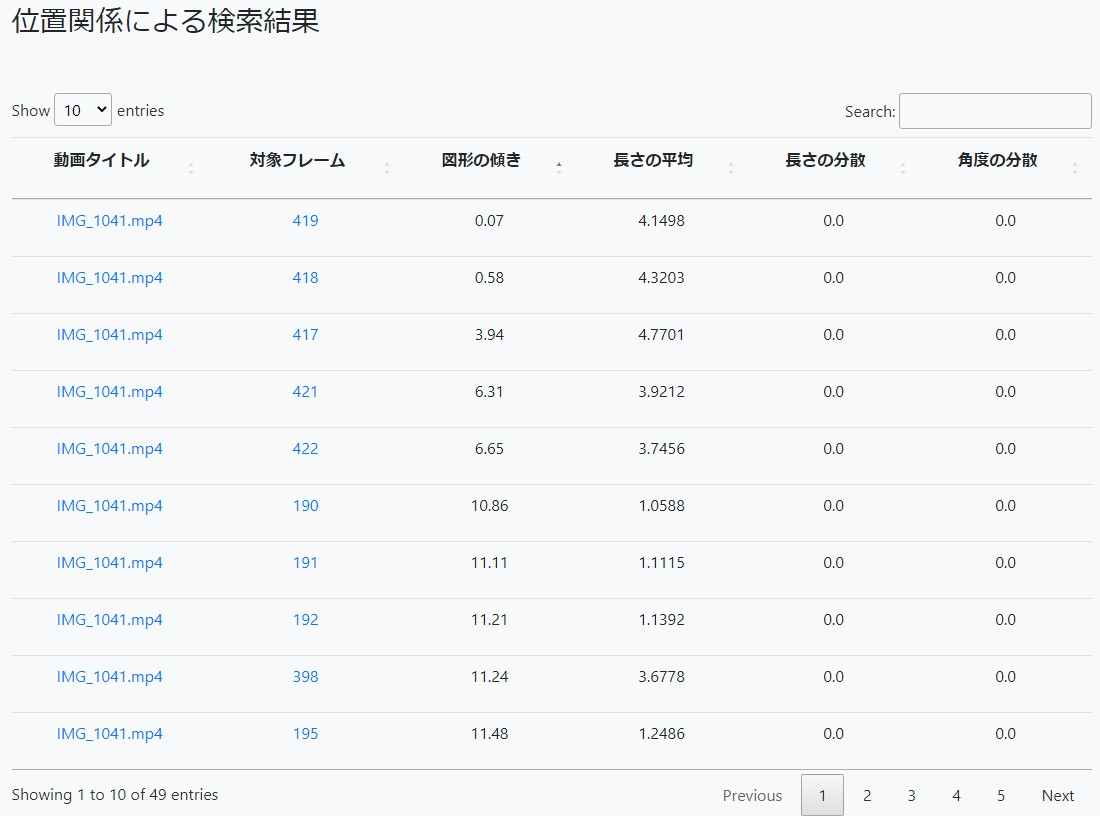
\includegraphics[width=13cm]{image/result_2_2_2.jpg}
  \caption{図\ref{fig:img_2-2-1}の検出結果(ソート:図形の傾き)}}
  \label{fig:img_2-2-2}
\end{figure}

\begin{figure}[H]
  \centering
<<<<<<< HEAD
  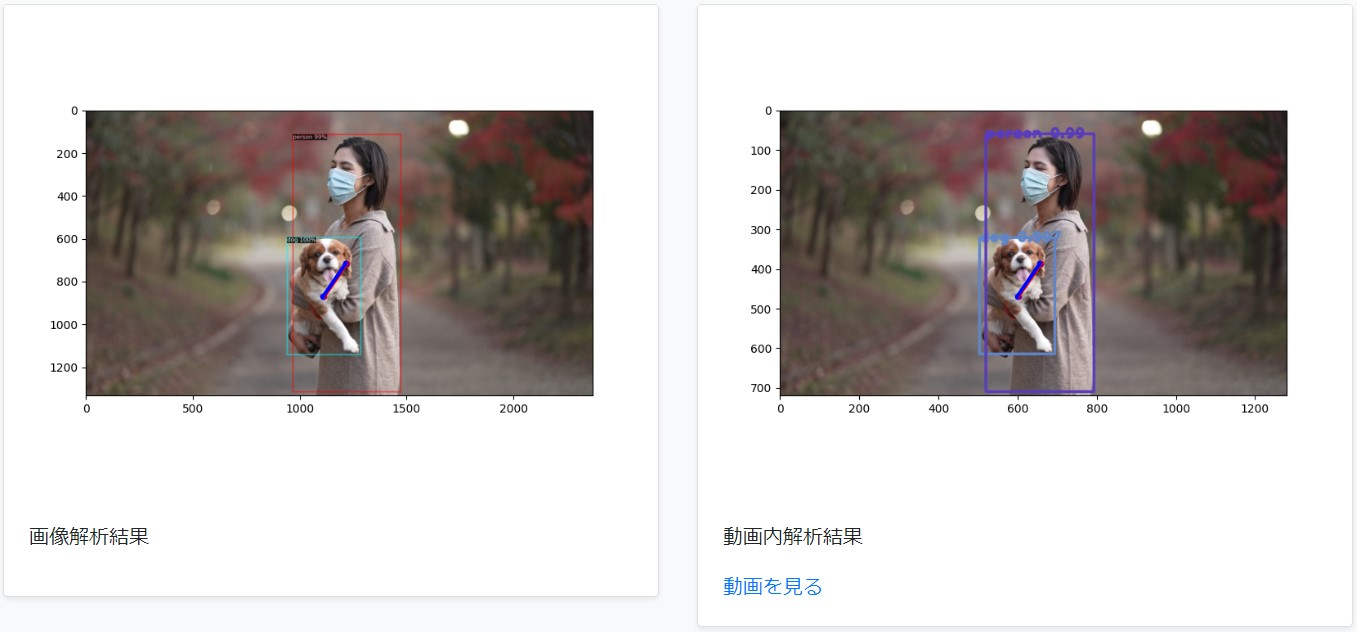
\includegraphics[width=13cm]{image/result2_2_4.jpg}
  \caption{動画タイトルの異なっているフレーム番号292}
  \label{fig:img_2_2_4}
\end{figure}

図\ref{fig:img_2_2_3}では,犬と女性がレンズに近づいているシーンが検出されている.
女性と犬の図形関係で,赤い線と蒼井線(入力画像の図形と検出された図形の関係)の角度がほとんど一致しており,入力した画像とほぼ同じ構図のシーンが検出されている.
図\ref{fig:img_2_2_3}の2枚の画像をよく比較してみると,女性の会と犬の重なりが少し違っていたり,犬の顔の位置が少し違っていたりする.
しかし,2つのオブジェクトの位置関係がほぼ同じであるため,類似シーンとして検出された.

図\ref{fig:img_2_2_4}では,入力された画像とほぼ一致しているシーンが検出されている.
こちらの画像は,入力画像との相違点が見られない.
オブジェクトの位置情報を用いた検索でも検出されそうなシーンでも,入力画像とフレームの類似度を計算して出力されている.

このように,解析したすべての動画の中から,幅広く類似シーンの検出を行なっていることがわかる.

\subsection{特殊な検索方法}
次に,本システムの位置関係を用いた検索でしか出来ない検索方法で類似シーンの検索を行う.
図\ref{fig:img_2_3}に示すように,動画中から欲しいシーンの構図を手作りした画像で検索を行ってみる.
この画像は,オブジェクト間の位置関係がある程度一致していれば,厳密でなくても動画中から類似するシーンの検索が可能となる.
なお,図\ref{fig:img_2_3}では,少年が手を振っている前を車が通過するシーンを動画中から検索するためにPowerPointで作成した画像である.
\begin{figure}[H]
  \centering
  \fbox{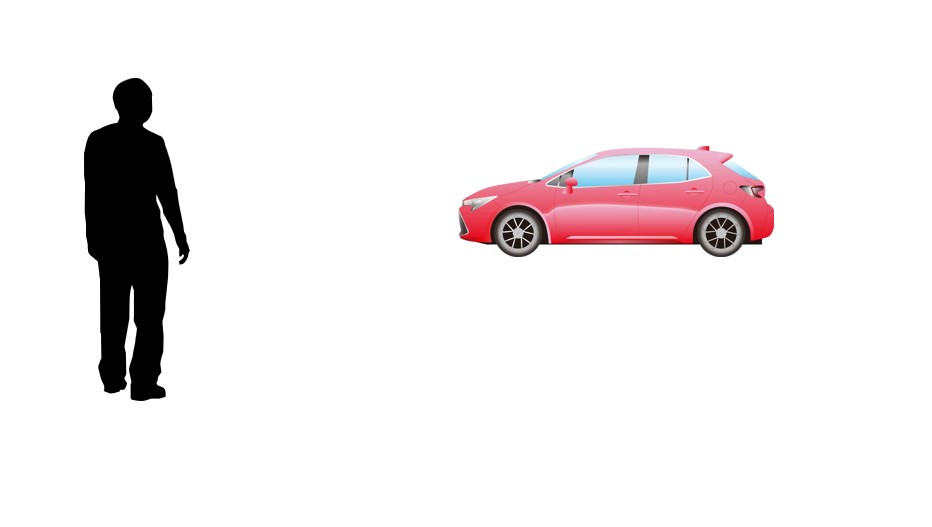
\includegraphics[width=13cm]{image/result_2_3.jpg}}
  \caption{入力画像}
  \label{fig:img_2_3}
\end{figure}

検索結果を表\ref{tab:tab_2_3}に示す.
\begin{table}[b]
  \centering
  \caption{図\ref{fig:img_2_3}の検出結果(【図形の傾き】で昇順ソート)}
  \label{tab:tab_2_3}
  \begin{tabular}{cccccc}
    \toprule
    \thead{動画タイトル} & \thead{対象フレーム} & \thead{図形の傾き} & \thead{長さの平均} & \thead{長さの分散} & \thead{角度の分散} \\
    \midrule
    道路沿い.mp4 & 419 & 0.07 & 4.1498 & 0.0 & 0.0 \\
    道路沿い.mp4 & 418 & 0.58 & 4.3203 & 0.0 & 0.0 \\
    道路沿い.mp4 & 417 & 3.94 & 4.7701 & 0.0 & 0.0 \\
    道路沿い.mp4 & 421 & 6.31 & 3.9212 & 0.0 & 0.0 \\
    道路沿い.mp4 & 422 & 6.65 & 3.7456 & 0.0 & 0.0 \\
    道路沿い.mp4 & 190 & 10.86 & 1.0588 & 0.0 & 0.0 \\
    道路沿い.mp4 & 191 & 11.11 & 1.1115 & 0.0 & 0.0 \\
    道路沿い.mp4 & 192 & 11.21& 1.1392 & 0.0 & 0.0 \\
    道路沿い.mp4 & 398 & 11.24 & 3.6778 & 0.0 & 0.0 \\
    道路沿い.mp4 & 195 & 11.48 & 1.2486 & 0.0 & 0.0 \\
    \bottomrule
  \end{tabular}
\end{table}

なお,位置情報を用いた検索では検索結果が出力されなかった.

表\ref{tab:tab_2_3}に示すように,図形の傾きが一番近いものは,図\ref{fig:img_2_3_1}である.

\begin{figure}[H]
  \centering
  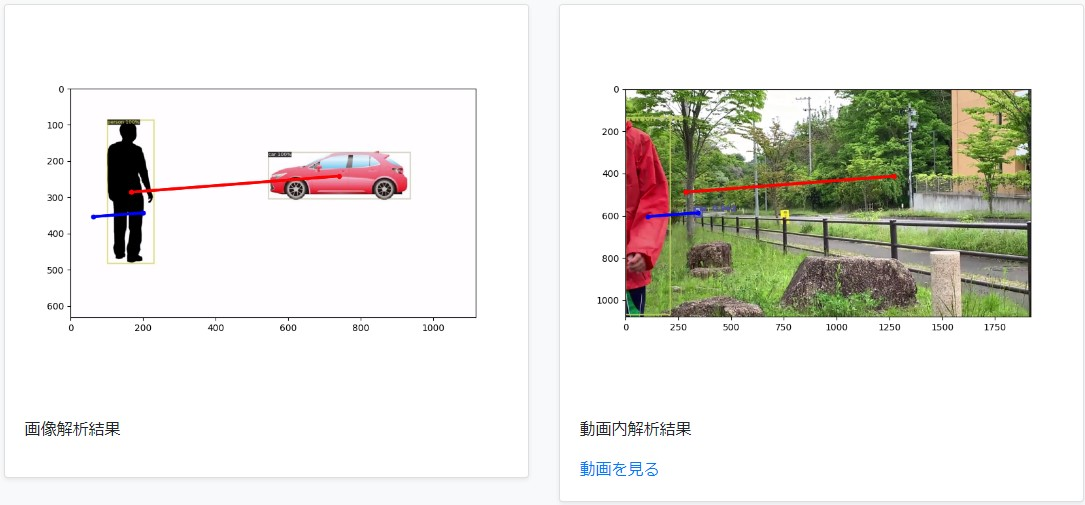
\includegraphics[width=13cm]{image/result_2_3_1.jpg}
  \caption{図\ref{fig:img_2_2_1}のベストマッチシーン(ソート:図形の傾き)}
  \label{fig:img_2_3_1}
=======
  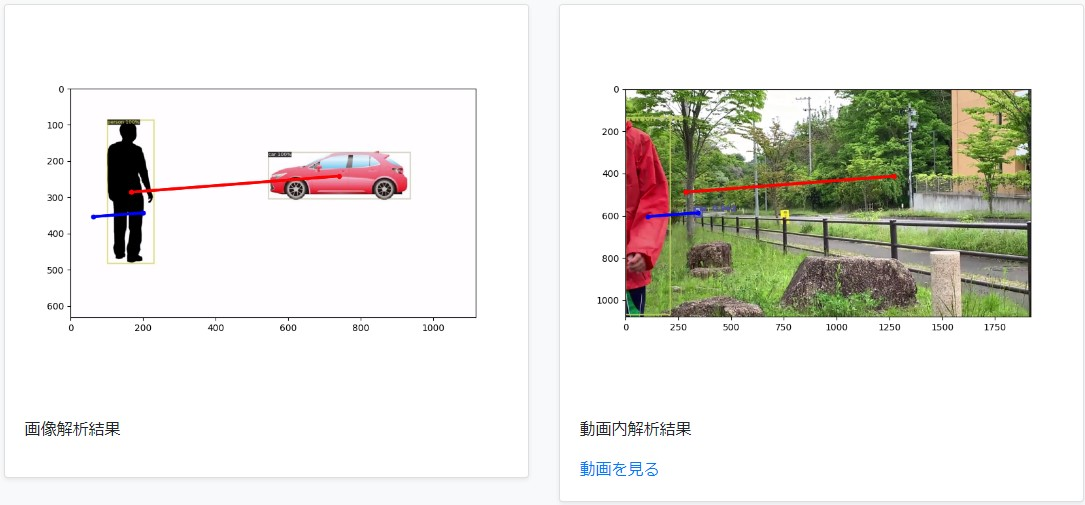
\includegraphics[width=13cm]{image/result_2_2_3.jpg}
  \caption{図\ref{fig:img_2-2-1}のベストマッチシーン(ソート:長さの平均)}
  \label{fig:img_2-2-3}
>>>>>>> parent of 36117c4 (考察増やした)
\end{figure}

2つのオブジェクトを結ぶ線分の傾きがほぼ一致しており,類似シーンとして出力された.
オブジェクトの位置関係の傾きが一番近いものを抽出したい場合は,図\ref{fig:img_2-2}で傾きを意識して検索することで,類似シーンを得ることができる.

また,図\ref{fig:img_2-2-4}に示すように,長さの平均が一番近いものは,図\ref{fig:img_2-2-5}である.
\begin{figure}[b]
  \centering
<<<<<<< HEAD
  \caption{図\ref{fig:img_2_3}の検出結果(【長さの平均】で昇順ソート)}
  \label{tab:tab_2_4}
  \begin{tabular}{cccccc}
    \toprule
    \thead{動画タイトル} & \thead{対象フレーム} & \thead{図形の傾き} & \thead{長さの平均} & \thead{長さの分散} & \thead{角度の分散} \\
    \midrule
    道路沿い.mp4 & 189 & 14.19 & 1.006 & 0.0 & 0.0 \\
    道路沿い.mp4 & 190 & 10.86 & 1.0588 & 0.0 & 0.0 \\
    道路沿い.mp4 & 191 & 11.11 & 1.1115 & 0.0 & 0.0 \\
    道路沿い.mp4 & 192 & 11.21 & 1.1392 & 0.0 & 0.0 \\
    道路沿い.mp4 & 193 & 11.5 & 1.1931 & 0.0 & 0.0 \\
    道路沿い.mp4 & 195 & 11.48 & 1.2486 & 0.0 & 0.0 \\
    道路沿い.mp4 & 196 & 11.71 & 1.2752 & 0.0 & 0.0 \\
    道路沿い.mp4 & 197 & 12,05 & 1.3159 & 0.0 & 0.0 \\
    道路沿い.mp4 & 198 & 12.44 & 1.3857 & 0.0 & 0.0 \\
    道路沿い.mp4 & 199 & 12.68 & 1.4449 & 0.0 & 0.0 \\
    \bottomrule
  \end{tabular}
\end{table}
=======
  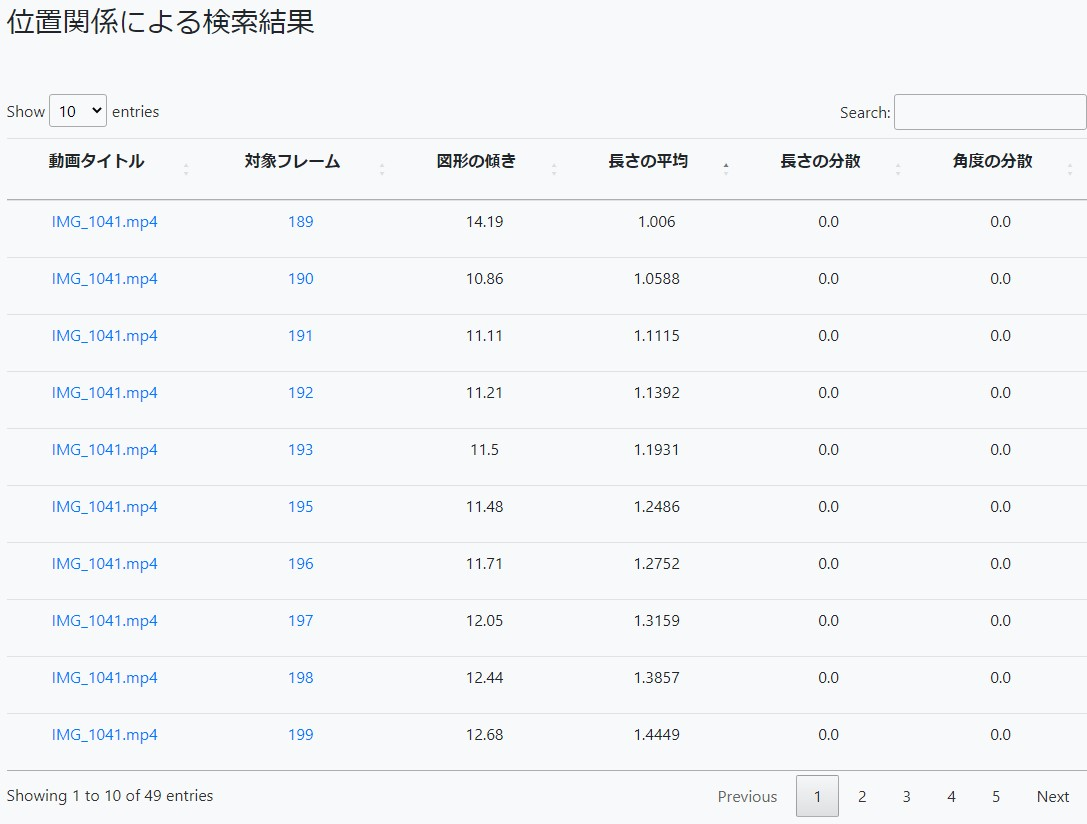
\includegraphics[width=13cm]{image/result_2_2_4.jpg}
  \caption{図\ref{fig:img_2-2-1}の検出結果(ソート:長さの平均)}
  \label{fig:img_2-2-4}
\end{figure}
>>>>>>> parent of 36117c4 (考察増やした)

\begin{figure}[H]
  \centering
  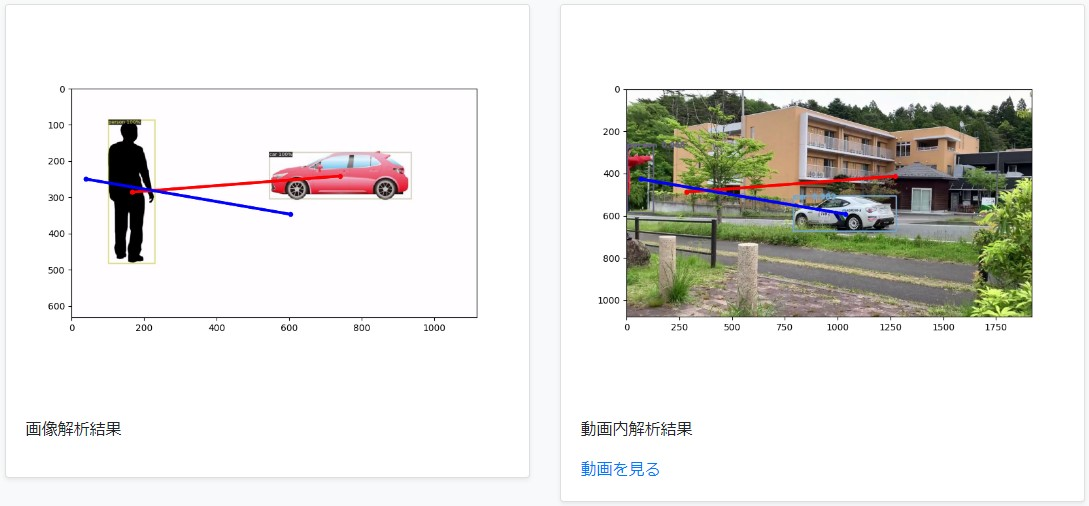
\includegraphics[width=13cm]{image/result_2_2_5.jpg}
  \caption{図\ref{fig:img_2-2-1}のベストマッチシーン(ソート:長さの平均)}
  \label{fig:img_2-2-5}
\end{figure}

2つのオブジェクトの長さの平均がほぼ一致しており,類似シーンとして出力された.
スポーツカーが人の前を通過しているシーンが出力されている.

<<<<<<< HEAD
なお,検索の目的であった,少年がスポーツカーに対して手を振っているシーンは,表\ref{tab:tab_2_4}中の,フレーム番号193あたりで見つけることができた(図\ref{fig:img_2_3_3}).
\begin{figure}[H]
=======
なお,検索の目的であった,少年がスポーツカーに対して手を振っているシーンは,図\ref{fig:img_2-2-4}中の,フレーム番号193あたりで見つけることができた(図\ref{fig:img_2-2-6}).
\begin{figure}[b]
>>>>>>> parent of 36117c4 (考察増やした)
  \centering
  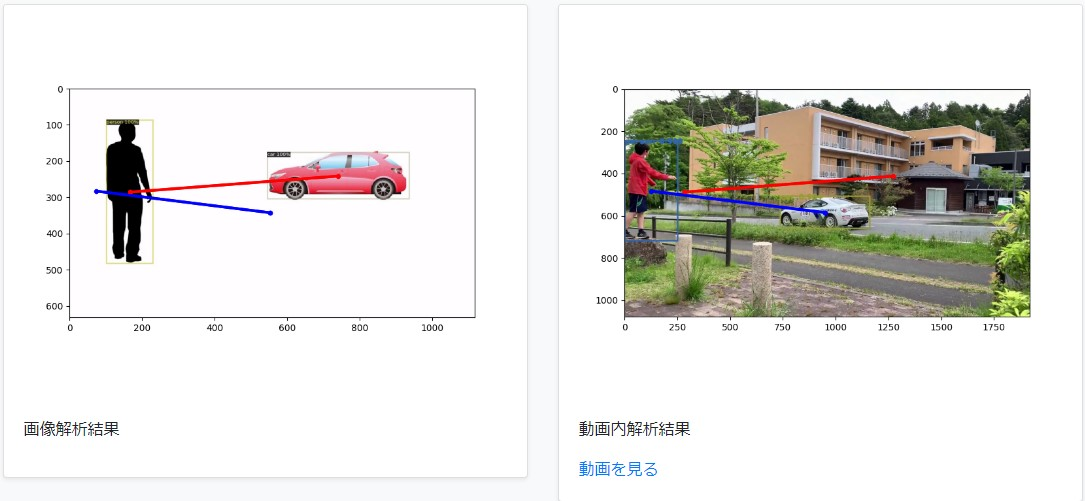
\includegraphics[width=13cm]{image/result_2_2_6.jpg}
  \caption{目的のシーン}
  \label{fig:img_2-2-6}
\end{figure}

このような目的のシーンのオブジェクト構成がある場合は,そのシーンを動画の中から検索することが可能となっている.

<<<<<<< HEAD
\begin{figure}[H]
  \centering
  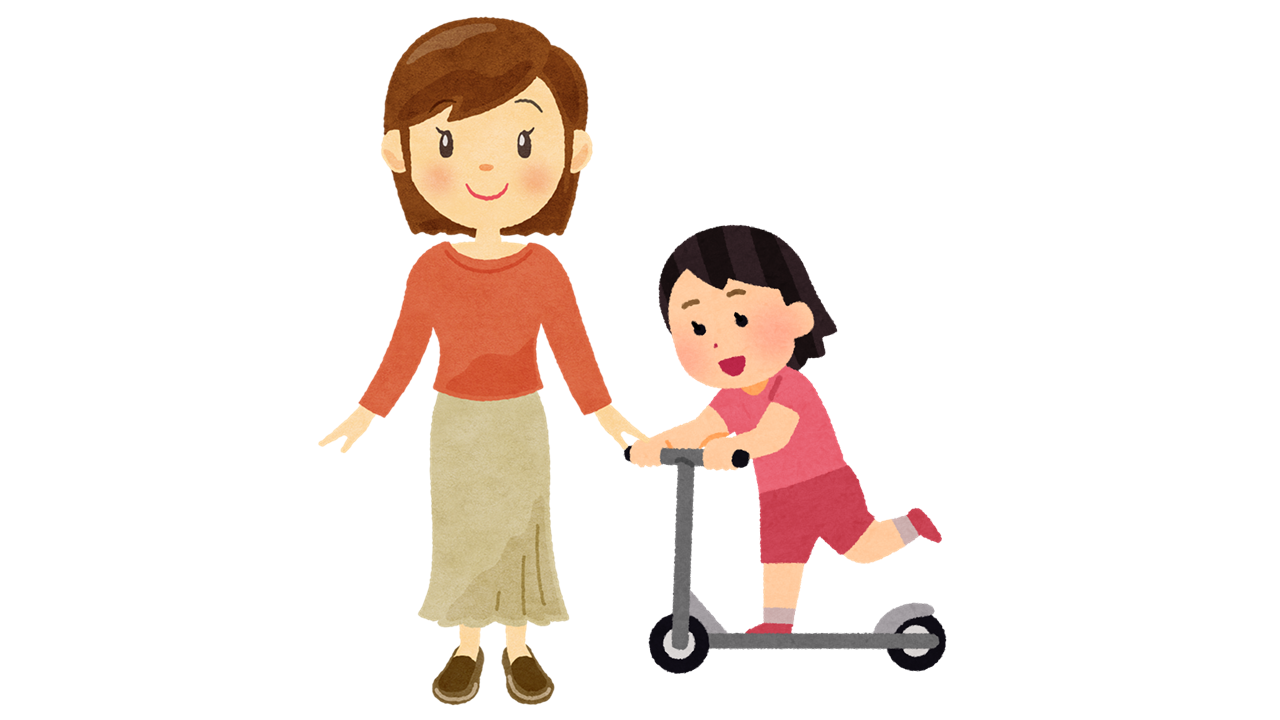
\includegraphics[width=13cm]{image/result_2_4.PNG}
  \caption{PowerPointで作成した入力画像}
  \label{fig:img_2_4}
\end{figure}


この画像を入力として検索してみたところ,結果は出力されなかった.
図\ref{fig:movie1}の動画がどういった解析で何が検出されているのかを調べたところ,表\ref{tab:tab_2_5}のようになっていた.
\begin{table}[b]
  \centering
  \caption{図\ref{fig:img_2_4}の解析結果}
  \label{tab:tab_2_5}
  \begin{tabular}{cc}
    \toprule
    \thead{オブジェクト名} & \thead{認識率[\%]}  \\
    \midrule
    person & 99.94 \\
    person & 99.9 \\
    skateboard & 98.26 \\
    \bottomrule
  \end{tabular}
\end{table}

他のフレームでも基本的に同様の結果となった.
そのため,personとskateboardを使った画像を入力にした場合に,類似シーンが検索されると考えられる.
図\ref{fig:img_2_4_2}のように,personとskateboardを使用した画像を入力にした結果,表\ref{tab:tab_2_6}のようになった.

\begin{figure}[H]
  \centering
  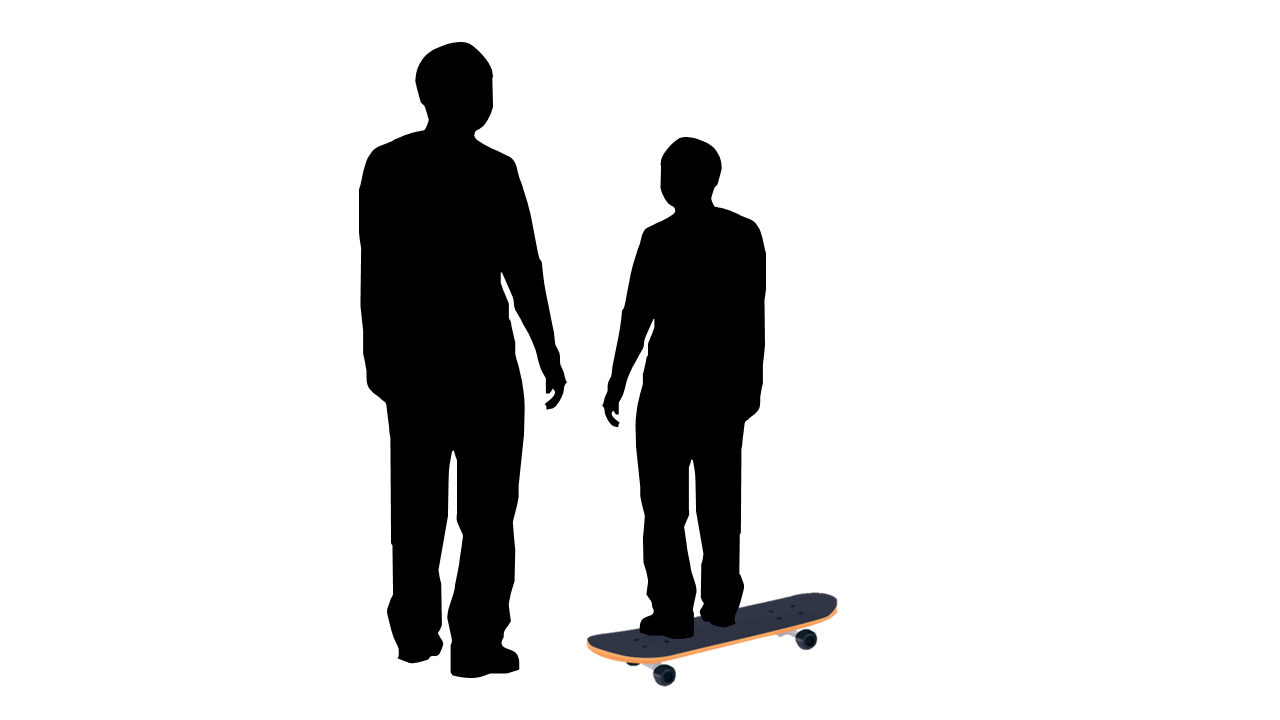
\includegraphics[width=13cm]{image/result_2_4_2.PNG}
  \caption{PowerPointで作成した入力画像}
  \label{fig:img_2_4_2}
\end{figure}

\begin{table}[b]
  \centering
  \caption{図\ref{fig:img_2_4_2}の検出結果(【図形の傾き】で昇順ソート)}
  \label{tab:tab_2_6}
  \begin{tabular}{cccccc}
    \toprule
    \thead{動画タイトル} & \thead{対象フレーム} & \thead{図形の傾き} & \thead{長さの平均} & \thead{長さの分散} & \thead{角度の分散} \\
    \midrule
    production ID\_4265040.mp4 & 356 & 8.25 & 1.1921 & 0.0055 & 10.7487 \\
    production ID\_4265040.mp4 & 357 & 8.58 & 1.2108 & 0.0071 & 10.8384 \\
    production ID\_4265040.mp4 & 358 & 8.67 & 1.224 & 0.0114 & 13.5234 \\
    production ID\_4265040.mp4 & 355 & 7.445 & 1.1973 & 0.0043 & 13.7131 \\
    production ID\_4265040.mp4 & 352 & 6.385 & 1.1459 & 0.0022 & 15.7873 \\
    production ID\_4265040.mp4 & 354 & 6.98 & 1.1819 & 0.0004 & 17.1475 \\
    production ID\_4265040.mp4 & 359 & 8.895 & 1.2697 & 0.0164 & 17.6553 \\
    production ID\_4265040.mp4 & 345 & 5.655 & 1.0659 & 0.0014 & 17.9837 \\
    production ID\_4265040.mp4 & 353 & 6.73 & 1.1585 & 0.0034 & 18..0178 \\
    production ID\_4265040.mp4 & 344 & 5.655 & 1.0544 & 0.0028 & 18.629 \\
    \bottomrule
  \end{tabular}
\end{table}

表\ref{tab:tab_2_6}のように,多くの類似シーンの検出ができた.
図形の傾きが一番小さい356フレーム目の検出結果を図\ref{fig:img_2_4_3}に示す.
\begin{figure}[H]
  \centering
  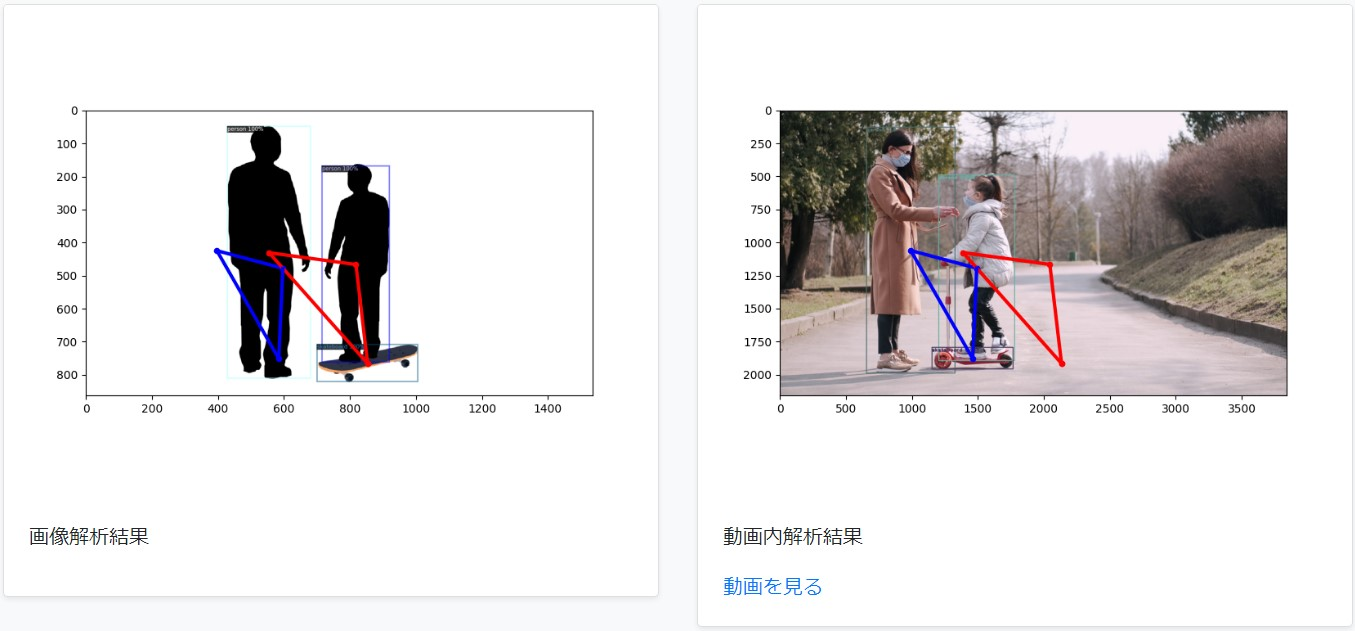
\includegraphics[width=0.5\textwidth]{image/result_2_4_3.jpg}
  \caption{図\ref{fig:img_2_4}の検出結果(フレーム番号:356)}
  \label{fig:img_2_4_3}
\end{figure}

このように,動画内に目的のシーンのオブジェクト構成がわかる場合は,そのシーンを動画の中から検索することが可能となっている.

\subsection{考察}
画像に一致している動画だけでなく,画像および動画内のオブジェクトの関係性を考慮して検索を行うことで,より幅広い検索が可能となった.

しかし,充分に使いやすい機能とは言えないと考える.
それは,検索結果の出力である.

図\ref{fig:img_2_3}での検索結果が非常にわかりずらい.
何でソートすると最も類似したシーンになるのか,目的のシーンになるのかが不明瞭であるためである.
現在,ソート機能では,図形の傾きや角度の分散など,1項目に限って行える.
しかし,ある場面では角度の分散と長さの平均の2項目をソートに利用したい場合もある.
こういった場面に対応できていないため,検索結果の出力については改善の余地があると考える.

また,図\ref{fig:img_2_3}のような,検出されたオブジェクト数が2つ場合は,3つ以上と比べて検索機能が不十分であると考える.
3つ以上のオブジェクト時には,必ずオブジェクト関係間で内角が存在するため,内角の分散を考慮することができる.
しかし,2つのオブジェクトの場合は,内角が存在しないため,内角の分散を考慮することができない.
また,辺も1つしかないため,辺の長さの分散も考慮することができない.
そのため,2つのオブジェクトの場合は,図形の傾きと長さの平均のみしか考慮できず,目的のシーンの検索が難しいと考える.
オブジェクトが1つの場合は,図形の傾き,長さの平均,長さの分散,角度の分散の全てを計算することができず,類似シーンの検索には,オブジェクト名の一致のみが考慮される.
これらの問題点を解決するために,オブジェクト数に応じて,検索機能を改善する必要があると考える.

オブジェクトが大量に画像内に存在する場合の,図形の計算についても考察する.
本システムの図形の計算では,\ref{sec:search_relationship}で説明したとおりである.
図形のオブジェクトを描画するために,オブジェクトの点を全て通りながら外周を描くようなルートを計算している.
オブジェクトの数が少ない場合は,図\ref{fig:img_2_4_4}のように,図形が正しく描画できる.
\begin{figure}[H]
  \centering
  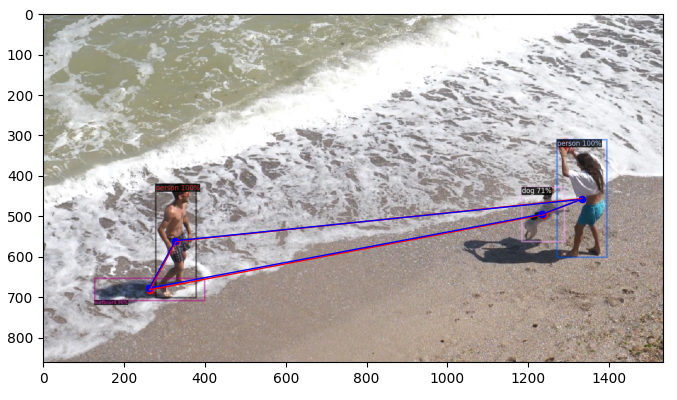
\includegraphics[width=0.5\textwidth]{image/result_2_4_4.png}
  \caption{オブジェクトが4つの図形の描画}
  \label{fig:img_2_4_4}
\end{figure}

しかし,オブジェクトが9個ある場合,図\ref{fig:img_2_4_5}のように,図形が正しく描画されていない.
\begin{figure}[H]
  \centering
  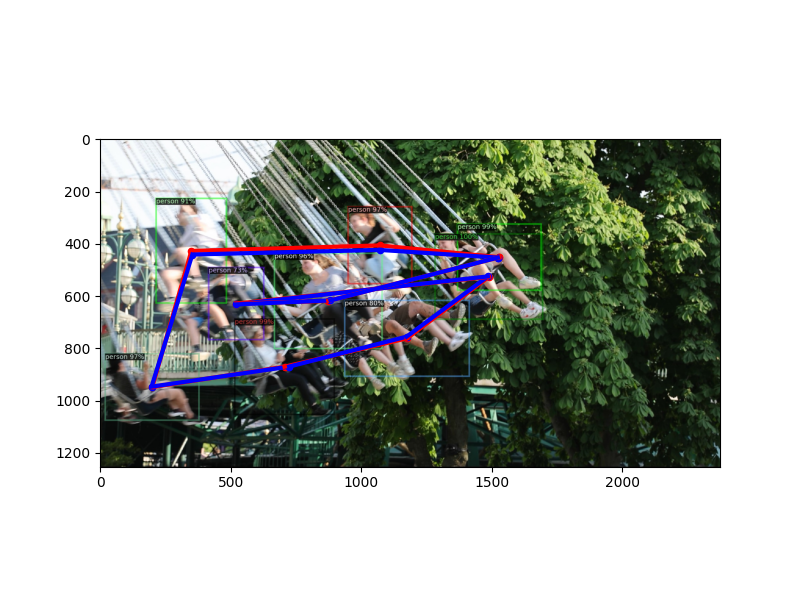
\includegraphics[width=0.5\textwidth]{image/result_2_4_5.png}
  \caption{オブジェクトが9つの図形の描画}
  \label{fig:img_2_4_5}
\end{figure}

図形が図\ref{fig:img_2_4_4}のように単純な図形であれば本システムの図形の計算でも問題ないが,
複雑な図形の場合は正しく図形を描画することができないことがあることがわかった.

類似シーンの検索精度向上には,この図形の計算の改善が必要であると考える.

\section{全体を通しての考察}

繰り返し本システムを利用した結果,検索結果の表示までにかかる時間が長いことが分かった.

データベースと処理時間の関係について検証を行った.
まず,動画解析にかかる時間を調べた.
その結果を図\ref{fig:img_2_5}に示す.
\begin{figure}[H]
  \centering
  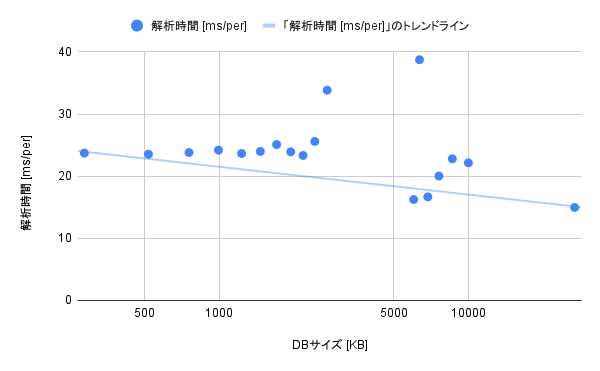
\includegraphics[width=0.5\textwidth]{image/result_2_5.png}
  \caption{DBサイズと検出時間の関係}
  \label{fig:img_2_5}
\end{figure}

図\ref{fig:img_2_5}の横軸には対数をとったデータベースのサイズを,縦軸には動画解析にかかる時間を示す.
動画解析の結果をデータベースに登録する際には,データベースのサイズに関わらず,オブジェクトあたりの解析時間はほぼ一定であることがわかった.

次に,検索時間について調べた.
位置情報を使用した検索にかかる時間を図\ref{fig:img_2_5_2}に,位置関係を使用した検索にかかる時間を図\ref{fig:img_2_5_3}に示す.
検索には画像内のオブジェクト数が異なる2種類の画像を使用した.
1枚目の画像は,画像内に3つのオブジェクトが存在する.
2枚目の画像は,画像内に8つのオブジェクトが存在する.
これにより,オブジェクト数によって検索時間がどのように変化するかもを調べた.
\begin{figure}[H]
  \centering
  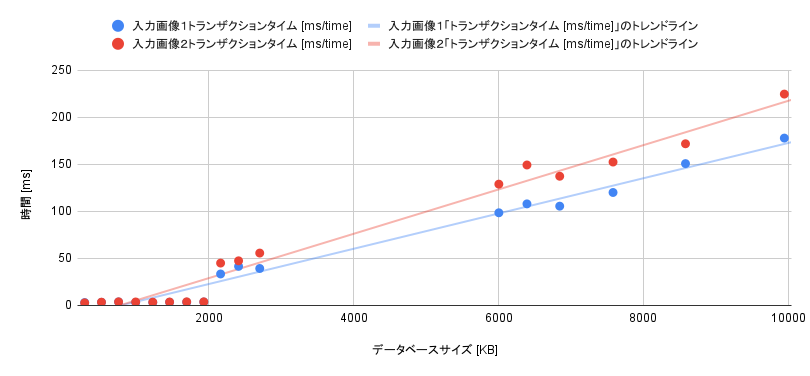
\includegraphics[width=0.5\textwidth]{image/result_2_5_2.png}
  \caption{DBサイズと検索時間の関係(位置情報を使用)}
  \label{fig:img_2_5_2}
\end{figure}

\begin{figure}[H]
  \centering
  \includegraphics[width=0.5\textwidth]{image/result_2_5_3.png}
  \caption{DBサイズと検索時間の関係(位置関係を使用)}
  \label{fig:img_2_5_3}
\end{figure}

図\ref{fig:img_2_5_2},図\ref{fig:img_2_5_3}の横軸はデータベースのサイズ,縦軸はデータベースにアクセスする時間をアクセスした回数で割った『1データを取得するのにかかる時間(トランザクションタイム)』である.
トランザクションタイムの計算式は,以下の通りである.
\begin{equation}
  トランザクション時間[ms] = \frac{データベースにアクセスした時間[ms]}{データベースにアクセスした回数[times]}
\end{equation}

これらの図を見ると,データベースのサイズが増加すると,データベースにアクセスする時間(トランザクションタイム)が増加していることがわかった.
特に,データベースのサイズが2,000KBまではトランザクションタイムが非常に短い.
その後は,サイズに比例してトランザクションタイムが急激に増加している.
また,画像内のオブジェクトの数によって,トランザクションタイムが変化していることがわかった.
図\ref{fig:img_2_5_2},図\ref{fig:img_2_5_3}とも,画像内のオブジェクト数が少ない方がトランザクションタイムが短い.

位置情報や位置関係を使用した検索方法別のトランザクションタイムの比較,どちらもあまり差がないことがわかった.

以上のことから,動画解析にかかる時間はデータベースのサイズに関係なく一定であるが,動画検索にかかる時間はデータベースのサイズに比例して増加していることがわかった.

検索時間を減らすためには,データベースに保存するデータ数の削減や,データベースとやり取りを行う回数(トランザクション回数)の削減などを行う必要があると考える.

また,別の問題もある.
それは,学習済みオブジェクト検出モデルを使用しているため,そのモデルで検出できないオブジェクトがあると,検索結果に表示されないことである.
これは従来のRGB値やヒストグラムを使用した比較の時には生じない.
どのような映像であろうと,RGB値やヒストグラムを比較することで,同一シーンの瞬間を検索することができる.

しかし,今回使用している学習済みモデルは,\ref{sec:system}節でも触れているがCOCOデータセットを使用しているため,そのデータセットに含まれていないオブジェクトは検出できない.
オブジェクトが検出できないと,同一シーンだけでなく,類似シーンの検索結果も表示されない.

この問題を解決するには,目的にあった学習済みモデルを使用する必要がある.
例えば,ゲーム画面に特化した検索システムを構築する場合,ゲーム画面のデータセットを用いてモデルを学習させた方が検索システムの精度が向上すると考えられる.
また,将棋の駒を学習データとしてモデルを作成すると,将棋の特定の盤面を検索することも可能であると考える.

今回使用しているDetectron2には,カスタムデータセットから推論を行う機能があるため,アノテーションデータが用意できれば,オリジナルのモデルを作成することも可能である.

一般的な映像を検索するシステムの構築を目標とした本研究では,Detectron2の学習済みモデルを使用しているが,今後は目的に合わせた学習済みモデルを使用することで,より高い精度の検索システムを構築することができると考える.
=======
>>>>>>> parent of 36117c4 (考察増やした)

\section{まとめ}
位置情報を用いた検索システムと,位置関係を用いた検索システムのそれぞれの動作と結果について考察を行った.


\chapter{結論}
\label{sec:conclusion}
本研究では,オブジェクト検出を用いた方法で動画検索システムを構築することができた.
また,さまざまな画像を用いて検索の評価を行った.
オブジェクトが多い時や,オブジェクトの位置関係が複雑な時には,検索の精度が低下することがわかった.
しかし,通常の検索方法ではできないような,オブジェクトの位置関係を考慮した検索が可能となった.

今後の課題として,検索性能や検索速度向上なども必要だということがわかった.
また,検索の精度を向上させるために,オブジェクトを認識させるためのモデルを改良したり,認識率のパラメータを変えることで,より精度の高い検索が可能となると考えられる.

\clearpage


\chapter{使用方法}
\label{sec:usage}
本システムの使用方法について説明する.
手順は大きく2つに分かれており,動画を解析するために事前に動画をアップロードすること,そして画像を用いた検索を行うことがそれぞれ必要となる.

\section{ユーザ登録}
本システムでは不特定多数のユーザができるようにするため,ユーザ情報が必要となっている.

ユーザ登録画面を図\ref{fig:user_register}に示す.

\begin{figure}[b]
  \centering
  \includegraphics[width=13cm]{image/user_register.jpg}
  \caption{ユーザ登録}
  \label{fig:user_register}
\end{figure}

登録にはユーザ名,メールアドレス,パスワードを入力する.

\section{ログイン}
ログイン画面を図\ref{fig:user_login}に示す.

\begin{figure}[b]
  \centering
  \includegraphics[width=13cm]{image/user_login.jpg}
  \caption{ログイン画面}
  \label{fig:user_login}
\end{figure}

ログインには,ユーザ登録時に登録したメールアドレスとパスワードを入力する.
正しくログインできると,トップ画面に遷移する.

\section{動画のアップロードについて}
本システムの動画検索機能を使用するには,検索前に動画をアップロードする必要がある.

アップロード画面に遷移するには,図\ref{fig:index}中の「動画登録」を選択する.

\begin{figure}[b]
  \centering
  \includegraphics[width=13cm]{image/index.jpg}
  \caption{動画アップロード画面遷移前}
  \label{fig:index}
\end{figure}

次に遷移後のアップロード画面を図\ref{fig:movie_upload}に示す.

\begin{figure}[b]
  \centering
  \includegraphics[width=13cm]{image/movie_upload.jpg}
  \caption{動画アップロード画面遷移後}
  \label{fig:movie_upload}
\end{figure}

その後,解析対象とする動画を選択し,アップロードを行う.
アップロードが正しく完了すると,自動的に動画リストに遷移し,解析が開始される.
複数の動画を解析対象にすることが可能だが,実際に同時には解析されず解析待ちという形で追加される.
なお,動画のアップロードが正しく完了していれば,解析待ちや解析中であってもブラウザを更新したり閉じたりしても動画には影響はない.

\section{画像を用いた検索について}
動画アップロードで解析まで完了した動画は,画像を用いた検索対象となる.検索手順について説明する.

トップ画面から検索画面に遷移する図\ref{fig:index}を示す.
検索には,類似シーンの検索の有無が選択できる.

トップ画面から画像検索を選択,動画を選択した時と同様に画像を選択すると図\ref{fig:image_upload}のようになる.

\begin{figure}[b]
  \centering
  \includegraphics[width=13cm]{image/image_upload.jpg}
  \caption{画像アップロード画面遷移後}
  \label{fig:image_upload}
\end{figure}


その後,検索ボタンを選択すると,検索が開始される.
検索が終了すると,図\ref{fig:search_result}結果が表示される.

\begin{figure}[b]
  \centering
  \includegraphics[width=13cm]{image/search_result.jpg}
  \caption{検索結果}
  \label{fig:search_result}
\end{figure}


この結果画面から,どの画像のどのシーン(フレーム)がどの程度類似しているかを確認することが可能になっている.
詳細な情報については,動画フレーム数のリンクから閲覧できる.ここでは,どのように認識されているかを確認でき,実際の動画を視聴することが可能となっている.

また,一度検索した画像は検索履歴として残っているため後から同じ画像を検索することが可能である.ヘッダー「画像検索履歴」を選択することで履歴が表示される.

\section{まとめ}
本章では,本システムの使用方法について説明した.

\clearpage

\chapter*{謝辞}
\addcontentsline{toc}{chapter}{謝辞}
本研究の実施の機会を与えてくださり,終始丁寧かつ的確な御指導,御鞭撻をいただきました准教授 藤原 和彦 氏に深謝の意を表し,厚く御礼申し上げます.\par
また,日常的に有益な議論をしていただいた研究室の皆様に感謝いたします.

\clearpage

\begin{thebibliography}{9}
\addcontentsline{toc}{chapter}{\bibname}
\bibitem{google_data} 月間6,500万ユーザーを超えたYouTube,2020年の国内利用実態──テレビでの利用も2倍に, Google https://www.thinkwithgoogle.com/intl/ja-jp/marketing-strategies/video/youtube-recap2020-2/
\bibitem{cnn} A Comprehensive Guide to Convolutional Neural Networks — the ELI5 way, Towards Data Science https://towardsdatascience.com/a-comprehensive-guide-to-convolutional-neural-networks-the-eli5-way-3bd2b1164a53
\bibitem{detectron2} Detectron2,Meta AI https://ai.facebook.com/blog/-detectron2-a-pytorch-based-modular-object-detection-library-/
\bibitem{coco} Microsoft COCO: Common Objects in Context, Microsoft https://cocodataset.org/

\end{thebibliography}

\end{document}
